%     ___                  
%    / _ \_______  ___  ___
%   / ___/ __/ _ \/ _ \(_-<
%  /_/  /_/  \___/ .__/___/
%               /_/        
% When eating fruit, remember the one who planted the tree.
% This Cheatsheet is a mix of @huandris, @jegraf and @smetzker. Expanded by me. \\
% Thank you for making my life way easier! 


%   _____          ____     
%  / ___/__  ___  / _(_)__ _
% / /__/ _ \/ _ \/ _/ / _ `/
% \___/\___/_//_/_//_/\_, / 
%                   /___/  
% Basic stuff
\documentclass[a4paper]{article}
\usepackage[utf8]{inputenc}
\usepackage[document]{ragged2e}
\usepackage[nswissgerman]{babel}
\usepackage{pgfplots}
\pgfplotsset{compat=newest}

%Tiny Font Sizes 
\usepackage{type1cm}
\usepackage[fontsize=9pt]{scrextend}

% Title Formatting
\usepackage{titlesec}
\titlespacing*{\section}
{0pt}{8pt}{2pt}
\titleformat{\section}
  {\normalfont\Large\bfseries\color{red}} % Formatting options
  {\thesection}{1em}{} % Label formatting

\titlespacing*{\subsection}
{0pt}{6pt}{2pt}
\titlespacing*{\subsubsection}
{0pt}{5pt}{1pt}

% 3 column landscape layout with fewer margins
\usepackage[landscape, left=0.05cm, top=0.05cm, right=0.05cm, bottom=0.5cm, footskip=0cm]{geometry}
\usepackage{flowfram}
\ffvadjustfalse
\setlength{\columnsep}{0.75cm}
\Ncolumn{3}
\linespread{0.9}

% Boxes: a base set, that is then customized
\usepackage[many]{tcolorbox}
\tcbset {
  base/.style={
    boxrule=0mm,
    leftrule=1mm,
    left=0.5mm,
    top=0.5mm,
    bottom=0.5mm,
    arc=0mm, 
    fonttitle=\small\bfseries, 
    colbacktitle=black!10!white, 
    coltitle=black, 
    toptitle=0.1mm, 
    bottomtitle=0mm,
    title={#1}
  }
}
 
%Define Boxes
\definecolor{blue}{rgb}{0.34, 0.7, 1}
\newtcolorbox{mainbox}[1]{
  colframe=blue, 
  base={#1}
}

\definecolor{green}{rgb}{0.2, 1, 0.4}
\newtcolorbox{howtobox}[1]{
  colframe=green, 
  base={#1},
}

\definecolor{purple}{rgb}{1, 0.3, 1}
\newtcolorbox{bspbox}[1]{
  colframe=purple, 
  base={#1}
}

\newtcolorbox{subbox}[1]{
  colframe=black!20!white,
  base={#1}
}

% Inline bullet points
\usepackage{paralist}
\setdefaultitem{$\textcolor{red}\bullet$}{$\textcolor{red}\circ$}{$\textcolor{red}\textasteriskcentered$}{$\textcolor{red}\textperiodcentered$}

% Redefine \epsilon to increase its size
\let\oldepsilon\epsilon
\renewcommand{\epsilon}{\text{\Large $\oldepsilon$}}

% Mathematical typesetting & symbols
\usepackage{amsthm, mathtools, amssymb, xfrac} 
\usepackage{marvosym, wasysym}
\usepackage{centernot}

% Tables
\usepackage{tabularx, multirow}
\usepackage{booktabs}
\renewcommand*{\arraystretch}{1.3}

% Make enumerations more compact
\usepackage{enumitem}
\setitemize{itemsep=0.5pt}
\setenumerate{itemsep=0.75pt}

% To include sketches
\usepackage{graphicx}
\usepackage[labelformat=empty]{caption}

% Tikz for drawings
\usepackage{tikz}

% Customize header
\usepackage{fancyhdr}
\usepackage{lastpage}
\pagestyle{fancy}
\renewcommand{\headrulewidth}{0pt}
\fancyfoot[L]{}
\fancyfoot[C]{\large \textbf{\thepage} / \pageref{LastPage}}
\fancyfoot[R]{jdickey, Analysis I - FS24}

% Math underline formulas
\usepackage{xcolor}
\newsavebox\MBox
\newcommand\Cline[2][red]{{\sbox\MBox{$#2$}%
  \rlap{\usebox\MBox}\color{#1}\rule[-1.2\dp\MBox]{\wd\MBox}{0.5pt}}}

% Metadata
\title{Analysis I Cheatsheet}
\author{jdickey}
\date{2024}

% Math helper stuff
\def\limn{\lim_{n\to \infty}}
\def\limxo{\lim_{x\to 0}}
\def\limxi{\lim_{x\to\infty}}
\def\limxn{\lim_{x\to-\infty}}
\def\sumk{\sum_{k=1}^\infty}
\def\sumn{\sum_{n=0}^\infty}
\def\dx{\text{ d}x}
\newcommand\N{\ensuremath{\mathbb{N}}}
\newcommand\R{\ensuremath{\mathbb{R}}}
\newcommand\Z{\ensuremath{\mathbb{Z}}}
\newcommand\Q{\ensuremath{\mathbb{Q}}}
\newcommand\C{\ensuremath{\mathbb{C}}}
\newcommand\notimplies{\centernot\implies}
\newcommand\notimpliedby{\centernot\impliedby}


% Image wrapping
\usepackage{wrapfig}
\setlength{\intextsep}{0pt plus 0pt minus 0pt} % more compact Imagewrapping

%                 __           __ 
%  _______  ___  / /____ ___  / /_
% / __/ _ \/ _ \/ __/ -_) _ \/ __/
% \__/\___/_//_/\__/\__/_//_/\__/ 
\begin{document}
\section{General}
\begin{wrapfigure}{r}{0.07\textwidth} 
  
\includegraphics[scale=0.1]{goodluckdoggo.png}
\end{wrapfigure}
Imagine how Function looks. Try inserting some pos. \& neg. values.
\begin{enumerate}[leftmargin=4.5mm, topsep=1pt, itemsep=1pt, parsep=1pt]
  \item Bestandteile der Aufgabe erkennen.
  \item Zugehörige Teile des Spicks lesen \\
        $\exists$ Fact i can use? $\exists$ Beispielbeweis?
  \item Referenzfolgen und Tabellen prüfen
\end{enumerate}
\textit{Calm and structured approach yields best results.}
Box: \colorbox{blue}{\color{black}Facts} \quad \colorbox{green}{\color{black}Vorgehen} \quad \colorbox{purple}{\color{black}Example}

$\mathbb{N} = \{ \textbf{0}, 1, 2, ... \}$ \quad $A \cap B = \{ x : x \in A \land x \in B \} $ 
  \tiny \color{gray} 
    (Schnitt)
  \color{black} \normalsize
$A \cup B = \{ x : x \in A \lor x \in B \} $
  \tiny \color{gray} 
    (Vereinigung)
  \color{black} \normalsize 


  \section{General}
  \subsection{Random}
  \begin{itemize}[leftmargin=4.5mm, topsep=1pt, itemsep=1pt, parsep=1pt]
    \item \textbf{gerade Funktion} hat Eigenschaft $f(-x)=f(x)$. Graph der Funktion ist symmetrisch zur yAchse. 
  \end{itemize}
  
  
  \subsection{Archimedisches Prinzip}
  \begin{wrapfigure}{r}{0.1\textwidth} 
    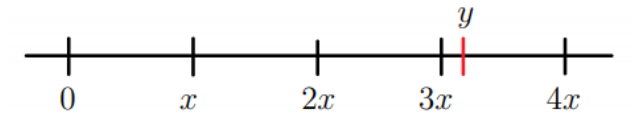
\includegraphics[scale=0.3]{archimedisches_Prinzip.png}
  \end{wrapfigure}
  
  \tiny \color{gray}
    = es gibt keine unendlich kleine oder unendlich grosse Zahlen
    -> $\forall y \in \R$ kann man durch wiederholte Addition eine grössere Zahl erreichen. \\
    -> $\forall y \in \R$ kann man durch wiederhotle Susbtraktion eine kleiner Zahl erreichen. \\
  \color{black} \normalsize
  Sei $x > 0 \in \R$ und $y \in \R$. $\exists n \in \mathbb{N}$ mit $y \leqslant n \cdot x$. \\
  
  \subsection{Intervalle}
  $]a,b[ = (a,b) = \{x \in \R \; | \; a < x < b\}$ 
    \tiny \color{gray}
      offenes Intervall
    \normalsize \color{black} \\
  $[a,b[ = [a,b) = \{x \in \R \; | \; a \leqslant x < b\}$ 
    \tiny \color{gray}
      halb-offenes Intervall
    \normalsize \color{black} \\
  $]a,b] = (a,b] = \{x \in \R \; | \; a < x \leqslant b\}$ 
    \tiny \color{gray}
      halb-offenes Intervall
    \normalsize \color{black} \\
  $[a,b] = [a,b] = \{x \in \R \; | \; a \leqslant x \leqslant b\}$ 
    \tiny \color{gray}
      abgeschlossenes Intervall
    \normalsize \color{black} \\
  Abgeschlossenes Intervall: $I \in \R$ ist abgeschlossen, wenn $\forall$ konvergente Folge $(a_n)_{n \geqslant 1}$ auch Grenzwert $\limn (a_n) \in$ I. \\
  
  \subsection{Beschränktheit, Schranken}
  $x$ ist die obere/untere Schranke. $A \in \R$ heisst 
  \begin{itemize}[leftmargin=4.5mm, topsep=1pt, itemsep=1pt, parsep=1pt]
    \item (v.o.b) von oben beschränkt: $\exists x \in \R$ s.t. $x \geqslant a$ $\forall a \in A$. \\
    \item (v.u.b) von unten beschränkt: $\exists x \in \R$ s.t. $x \leqslant a$ $\forall a \in A$. \\
    \item beschränkt: (v.o.b) und (v.u.b) \\
  \end{itemize}
  
  \subsection{Minimum, Maximum}
  Minimum: $x \in A$ ist und $x$ untere Schranke \\
  Maximum: $x \in A$ ist und $x$ obere Schranke
  
\subsection{Infimum \& Supremum}
\begin{mainbox}{ Infimum \& Supremum}
    \begin{wrapfigure}{r}{0.16\textwidth} 
      \centering
      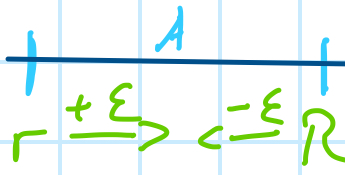
\includegraphics[scale=0.14]{infimumsupremum.jpeg}
    \end{wrapfigure}
    Sei $A \in \R$, $A \neq \emptyset$
    \begin{itemize}[leftmargin=4.5mm, topsep=1pt, itemsep=1pt, parsep=1pt]
      \item Infimum: grösste untere Schranke \\ $R := \inf A$ (falls $A$ v.u.b). \\      
        \color{gray} \small 
          $\forall a \in A : r \leqslant a$ \quad $\forall \epsilon > 0 \ \exists a \in A : a < r + \epsilon$ 
        \color{black} \normalsize
      \item Supremum: kleinste obere  Schranke \\ $R := \sup A$ (falls $A$ v.o.b). \\     
        \color{gray} \small 
          $\forall a \in A : a \leqslant R$ \quad $\forall \epsilon > 0 \ \exists a \in A : a > R - \epsilon$ 
        \color{black} \normalsize
    \end{itemize}
\end{mainbox}

  \begin{itemize}[leftmargin=4.5mm, topsep=1pt, itemsep=1pt, parsep=1pt]
    \item Wenn $x = \sup A$, so gilt $x \geqslant a \; \forall a \in A$ und all $y < x$ sind keine oberen Schranken.Falls $A$ ein Maximum hat, gilt $\max A = \sup A$.
    \item Wenn $A \subset B \subset R$ und $B$ beschränkt ist, so ist $A$ beschränkt und $\sup A \leqslant \sup B$, $\inf A  \geqslant \inf B$.
    \item  Für $A \neq \emptyset$ und nicht v.o.b. definieren wir \\
          $\sup A = \infty$, falls nicht v.u.b. $\inf A = -\infty$.
  \end{itemize}

\section{Folgen}
\subsection{Grundlagen}
\textbf{Folge} (reeler Zahlen) ist eine Abbildung $a: \mathbb{N}^* \longrightarrow \R$. \\
    $(a_n)_{n\geqslant1}$ = Folge \qquad $a_n$ = Element einer Folge \\
    \tiny \color{gray}
      Bsp. $(a_n)_{n\geqslant1} = \frac{1}{n}$: $a_1 = \frac{1}{1}, a_2 = \frac{1}{2}, ...$ \\
    \normalsize \color{black}

\subsection{Vorgehen}
\begin{howtobox}{Grenzwerte berechnen Folgen}
  \begin{itemize}[leftmargin=3mm, topsep=1pt, parsep=1pt]
    \item[1.] Grenzwert durch simple Operationen und Umformen berechnen?
    \item[2.] Trick anwenden? (Limes binom, - substitution, - Log)
    \item[3.] Grenzwert von Brüchen mit $n \to \infty$?:  \\
              Grösste Potenz von $n$ ausklammern und kürzen. Alle übrigen Brüche der Form $\frac{a}{n^s}$ oder $\frac{i}{n^s}$ streichen, da sie gegen 0 gehen für $n \rightarrow \infty$.
    \item[4.] Grenzwert von Wurzel $\pm$ smth. im Nenner berechnen? \\
              Multipliziere mit inversen des Nenners (oben \& unten).
    \item[5.] Berechne Grenzwert mit Sandwhich-Theorem.
    \item[6.] Rekursive Folge? Siehe Absatz Rekursive Folgen.
  \end{itemize}
\end{howtobox}

\begin{howtobox}{Konvergenzanalyse Folgen (Konv.? Div.?)}
  \begin{itemize}[leftmargin=3mm]
    \item[1.] Abschätzen: Nur grösste Terme prüfen. 
    \item[2.] Grenzwert zeigen per Definition der Konvergenz. (Vor allem für formale Beweise)
    \item[3.] Suchen eines konvergenten Majorant
    \item[4.] Cauchy-Kriterium 
  \end{itemize}
\end{howtobox}




\subsection{Konvergente Folge \& Limes}
Folge konvergiert wenn die Differenz zwischen Folgegliedern und Grenzwert immer kleiner wird.
\begin{mainbox}{Konvergente Folge \& Limes}
  \begin{itemize}[leftmargin=3mm, topsep=1pt, parsep=1pt]
    \item Folge $(a_n)_{n \geqslant 1}$ ist konvergent $\Leftrightarrow \exists l \in \R$ s.t. $\forall \epsilon > 0$ die Menge $\{n \in \mathbb{N}^*: a_n \notin \quad ]l - \epsilon, l + \epsilon[\}$ endlich ist. 
        $l = \lim a_n$. \\
      \tiny \color{gray}
        Eine Folge ist konvergent wenn egal welchen Abstand $\epsilon$ man wählt, nach endlichen Ausnahmeindizes $N$ alle weiteren Folgengliedern weniger als Abstand $\epsilon$ vom Grenzwert $l$ entfernt sind. 
        Also im Intervall ]$l - \epsilon, l + \epsilon[\}$." \\
      \normalsize \color{black}
    \item $(a_n)_{n \geqslant 1}$ konvergiert gegen $l = \limn (a_n) \\ \Leftrightarrow \forall \epsilon > 0 \; \exists N \geqslant 1$ so dass $|a_n - l| < \epsilon \; \forall n \geqslant N$ \\
      \tiny \color{gray}
        Folge konvergiert weil man differenz zwischen Folgegliedern \& Grenzwert beliebig klein machen kann in dem man n gross genug wählt. 
        $\rightarrow$ Es gibt immer einen Index N, ab welchem keine Ausnahmeindizes mehr auftreten. 
    \end{itemize}
\end{mainbox}
\begin{itemize}[leftmargin=4.5mm , topsep=0pt, parsep=0pt]
  \item konvergent $\Rightarrow$ beschränkt, aber $\nLeftarrow$ \\
  \item Reihenfolge hat keinen Einfluss auf Konvergenz. Tatsache, dass sich Glieder einem bestimmten Wert annähern, bleibt unverändert.
\end{itemize}

\begin{bspbox}{$\epsilon$-Konvergenz (Konvergenzbeweis)}
  \tiny \color{gray}
    Ab index N sind alle Glieder $(a_n)$ näher als $\epsilon$ am Grenzwert.
  \normalsize \color{black} \\
  Wähle beliebig kleines $\epsilon$ und zeige $N = N(\epsilon) \in \mathbb{N}$ existiert, so dass $\forall n \geqslant N$ gilt: \\ $|a_n - \limn (a_n)| = \dots < \epsilon$ \\ Löse nach $n$ auf und wähle $N := \lceil n \rceil$. Somit gilt $\forall n \geqslant N$, dass $|a_n - \limn (a_n)| \leqslant \epsilon$ (def $\limn$).
\end{bspbox}

\begin{bspbox}{Divergenz von Folgen}
  Divergente Folge = nicht konvergent = kein Grenzwert.
  \begin{itemize}[leftmargin=3mm, topsep=1pt, parsep=1pt]
    \item[1.] Suchen eines divergenten Minorant.
    \item[2.] \textbf{Alternierende Folgen} Zeige, dass \\ $\limn (a_{p1(n)}) \neq \limn (a_{p2(n)})$, z.B. bei einer Folge der Form $(-1)^n \cdot f(x)$.
  \end{itemize}
\end{bspbox}

\subsection{Rechenregeln zu Konvergenz \& G.W.}
Sei $(a_n)_{n \geqslant 1}$ und $(b_n)_{n \geqslant 1}$ konvergente Folgen mit $\limn (a_n) = a$ und $\limn (b_n) = b$.
\begin{itemize}[leftmargin=4.5mm, topsep=1pt, parsep=1pt]
  \item dann $(a_n + b_n)_{n \geqslant 1}$ konvergent \& $\limn (a_n + b_n) = a + b$  
  \item dann $(a_n \cdot b_n)_{n \geqslant 1}$ konvergent \& $\limn (a_n \cdot b_n) = a \cdot b$
  \item wenn $b_n \neq 0 \forall \geqslant 1 \land b \neq 1$ dann ist $\left(\frac{a_n}{b_n}\right)_{n \geqslant 1}$ konvergent und $\limn \left(\frac{a_n}{b_n}\right) = \frac{a}{b}$ 
\end{itemize}

\subsection{Monotone Folgen}
\begin{itemize}[leftmargin=3mm, topsep=1pt, parsep=1pt]
  \item monoton wachsend: $\forall n \in \mathbb{N}$ gilt, dass $a_n \leqslant a_{n + 1}$
  \item streng monoton wachsend: $\forall n \in \mathbb{N}$ gilt, dass  $a_n < a_{n + 1}$
  \item monoton fallend: $\forall n \in \mathbb{N}$ gilt, dass $a_n \geqslant a_{n + 1}$
  \item streng monoton fallend: $\forall n \in \mathbb{N}$ gilt, dass $a_n > a_{n + 1}$
\end{itemize}
\begin{bspbox}{Monotonie prüfen durch Ableitung}
  Ersetze $n$ durch $x$ und berechne die Ableitung nach $x$. Gilt $a'(x) \geqslant 0$, ist sie monoton wachsend und wenn $a'(x) \leqslant 0$ gilt, ist sie monoton fallend.
\end{bspbox}
Kann auch durch Induktionsbeweis gezeigt werden. Siehe "Grenzwert rekursiver Folgen berechnen"

\subsection{Sandwhich Theorem}
Grenzwert von Folge bestimmen, wenn sie zwischen zwei anderen Folgen mit gleichem, bereits bekannten Grenzwert liegt.
\begin{mainbox}{Sandwhich Theorem}
  Sei $\limn (a_n) = \alpha$, $\limn (b_n) = \alpha$ und \\ $a_n \leqslant c_n \leqslant b_n$, $\forall n \geqslant k$, dann gilt $\limn (c_n) = \alpha$.
\end{mainbox}

\subsection{Weierstrass}
Grenzwert von monotonen, beschränkten Folgen berechnen.
\begin{mainbox}{Weierstrass (Monotone Konv.satz)} 
  \begin{itemize}[leftmargin=3mm, topsep=1pt, parsep=1pt]
    \item Folge $(a_n)$ monoton wachsend $\&$ nach oben beschränkt \\
      $\Rightarrow \limn (a_n) = \sup\{a_n: n \geqslant 1\}$ \\
      \tiny \color{gray}
        Grenzwert ist supremum des Intervalls der Folge $a_n$ 
      \normalsize \color{black}
    \item Folge $(a_n)$ monoton fallend $\&$ nach unten beschränkt \\
          $\Rightarrow \limn (a_n) = \inf\{a_n: n \geqslant 1\}$ \\
      \tiny \color{gray}
        Grenzwert ist infimum des Intervalls der Folge $a_n$ 
      \normalsize \color{black}
  \end{itemize}
\end{mainbox}
\begin{wrapfigure}{r}{0.12\textwidth} 
  \centering
  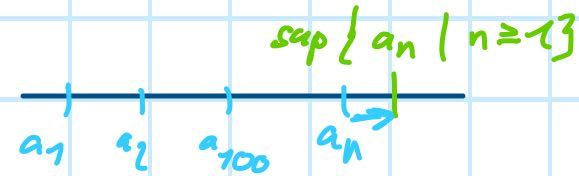
\includegraphics[scale=0.15]{weierstrass.jpg} 
\end{wrapfigure}
Example monoton wachsend: \\
\tiny \color{gray}
  Weierstrass darf auch angewendet werden, wenn Folge erst nach einem index N monton wachsend/fallend ist. 
\normalsize \color{black}
\\
\begin{itemize}[leftmargin=4.5mm, topsep=1pt, parsep=1pt]
  \item Folge $a_n$ monoton wachsend $\&$ nach oben \underline{un}beschränkt \\
        $\Rightarrow \limn (a_n) = \infty$ \\
  \item Folge $a_n$ monoton fallend $\&$ nach unten \underline{un}beschränkt \\
        $\Rightarrow \limn (a_n) = -\infty$ \\
\end{itemize}


\subsection{Limes Inferior/Superior}
\tiny \color{gray}
  Anwendung: Verhalten von nicht konvergenten Folgen analysieren durch definieren zweier monotonen Folgen welche zum kleinsten bzw. grössten Häufungspunkt konvergieren.  
\normalsize \color{black}
\begin{mainbox}{Limes Inferior/Superior}
  $(a_n)_{n \geqslant 1}$ beschränkt $\implies \exists M \in \R, \ \forall n \in \mathbb{N} : |a_n| < M$. \\
  Für $k \in \mathbb{N}$ existieren dann gemäss dem Satz von Sup und Inf $b_k = \inf_{n \geqslant k} (a_n) < \sup_{n \geqslant k} (a_n) = c_k$. Dann gilt: \\
  $-M \leqslant b_1 \leqslant\dots \leqslant b_{k + 1} \leqslant c_{k + 1} \leqslant \dots \leqslant c_1 \leqslant M$ \\
  Mit Satz für monotone Konvergenz folgt Existenz von lim sup \& lim inf:\\
  \begin{itemize}[leftmargin=3mm, topsep=1pt, parsep=1pt]
    \item Lim Inferior (kleinster Häufungspunkt): $\limn \inf(a_n) := \limn (b_k) = b$ \\
      \tiny \color{gray}
        = unterer Häufungspunkt der sich Folge annähert. 
      \normalsize \color{black}
  
    \item Lim Superior (grösster Häufungspunkt): $\limn \sup(a_n) := \limn (c_k) = c$ \\
      \tiny \color{gray}
        = oberer Häufungspunkt der sich Folge annähert.
      \normalsize \color{black}
    \end{itemize}
  \end{mainbox}
  Example: 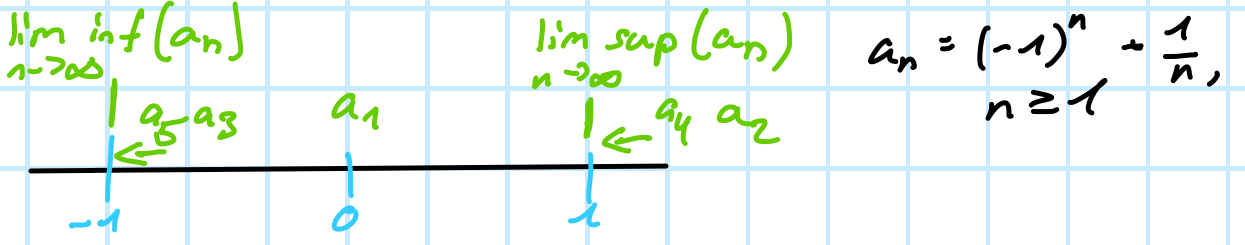
\includegraphics[scale=0.14]{limesinferiorsuperior.jpeg} \\
\begin{itemize}[leftmargin=4.5mm, topsep=1pt, parsep=1pt]
  \item $\limn \inf(a_n) > -\infty \Leftrightarrow (a_n)_{n \geqslant 1}$ nach unten beschränkt \\
  \item $\limn \sup(a_n) < \infty \Leftrightarrow (a_n)_{n \geqslant 1}$ nach oben beschränkt \\
  \item $\limn \inf(a_n) = \infty \Leftrightarrow (a_n)_{n \geqslant 1}$ konvergiert gegen $\infty$ \\
  \item $\limn \sup(a_n) = -\infty \Leftrightarrow (a_n)_{n \geqslant 1}$ konvergiert gegen $- \infty$ \\
  \item Sei $(a_n)_{n \geqslant 1}$ beschränkt. Dann $\forall \epsilon > 0: N \in \mathbb{N}$ s.t. $\forall n \leqslant N: a_n \in (\limn \inf a_n - \epsilon , \limn \sup a_n + \epsilon)$\\
\end{itemize}

\subsection{Cauchy-Kriterium/Cauchy-Folge}
Konvergenz einer Folge prüfen ohne Grenzwert zu kennen.

\begin{mainbox}{Cauchy-Kriterium}
  Folge $(a_n)$ konvergiert $\iff (a_n)_{n \geqslant 1}$ beschränkt und $\limn \inf(a_n) = \limn \sup(a_n)$ \\  
  \tiny \color{gray}
      Folge konvergiert weil die Differenz zwischen Folgegliedern mit wachsendem Index immer kleiner wird.  
  \normalsize \color{black} 
\end{mainbox}

\begin{mainbox}{Cauchy-Folge}
    $(a_n)$ heisst Cauchy-Folge falls  \\ $\forall \epsilon > 0, \ \exists N \in \mathbb{N}$: $|a_n - a_m| < \epsilon$ $\forall m,n \geq N$ \\
      \tiny \color{gray}
        Bei einer $Cauchy-Folge$ ist egal welchen Abstand $\epsilon$ man wählt, nach endlichen Ausnahmeindizes $N$ der Abstand zwischen \textit{beliebigen} Folgengliedern unter $\epsilon$. Daher ist sie konvergent.
      \normalsize \color{black} 
\end{mainbox}
\begin{itemize}[leftmargin=4.5mm, topsep=1pt, parsep=1pt]
  \item $(a_n)$ Cauchy-Folge $\Rightarrow (a_n)$ beschränkt
  \item  $(a_n)$ konvergent $\Leftrightarrow (a_n)$ Cauchy-Folge
  \item $(a_n)$ nicht Cauchy-Folge $\Rightarrow (a_n)$ divergent
\end{itemize}

\subsection{Teilfolge}
\begin{mainbox}{Teilfolge}
  Teilfolge $(b_n)_{n \geqslant 1}$ von $(a_n)_{n \geqslant 1}$ ist $b_n = a_{l(n)}$. \\
  $l(n)$ ist Indexfunktion mit Eigenschaft: $l(n) < l(n + 1)$ \\
  \tiny \color{gray}
    Bsp: $a_n = (-1)^n + \frac{1}{n}$. Sei $l(n) = 2n$. Teilfolge: $b_n = a_{2n} = (-1)^{2n} + \frac{1}{2n} = 1 + \frac{1}{2n}$
  \normalsize \color{black}
\end{mainbox}
\begin{itemize}[leftmargin=4.5mm, topsep=1pt, parsep=1pt]
    \item Entsteht durch weglassen von Folgengliedern.
    \item $(a_n)_{n \in \N}$ konvergent $\Rightarrow (a_{\text{l}(n)})_{n \in \N}$ konvergent $\forall$ Teilfolgen.
\end{itemize}

\subsection{Bolzano Weierstrass}
\begin{subbox}{Bolzano Weierstrass}
  Jede beschränkte Folge besitzt eine konvergente Teilfolge.
\end{subbox}
\begin{itemize}[leftmargin=4.5mm, topsep=1pt, parsep=1pt]
    \item $(a_n)_{n \in \N}$ beschränkt $\implies$ für jede beschränkte Teilfolge $(b_n)_{n \in \N}$ gilt $\liminf_{n \to \infty} a_n \le \lim_{n \to \infty} b_n \le  \limsup_{n \to \infty} a_n$
    \item Es gibt je eine Teilfolgen von $(a_n)_{n \in \N}$ die $\liminf_{n \to \infty} a_n$ resp. $\limsup_{n \to \infty} a_n$ als Limes annehmen.
\end{itemize}

\subsection{Rekursive Folgen (Induktiv definierte)}
Folgen können Rekrusiv definiert werden. Sei Folge $(a_k)_{k \geq 1}: \ a_1 = c, \ a_{k+1} = f(a_k), k \geq 1$
\begin{bspbox}{Grenzwert Rekursiver Folgen berechnen}
  Sei Folge $(a_k)_{k \geq 1}: \ a_1 = c, \ a_{k+1} = sin(a_k), k \geq 1$
  \begin{itemize}[leftmargin=3mm, topsep=1pt, parsep=1pt]
    \item[1.] Monotonie beweisen per Induktion \\
          $a_1 = c \land c \in [0, \pi] \implies a_1 \in [0, \pi]$ \\
          $sin(x) \leq x \ \forall x \geq 0 \implies a_{k+1} \leq a_k \implies $ monoton fallend
    \item[2.] Beschränktheit zeigen \\
          $sin(x) \geq 0 \ \forall x \in [0, \pi] \implies a_k \geq 0 \forall k \geq 1 \implies$ v.u.b \\
    \item[3.] Weierstrass Monoton Konvergenzsatz \\
          $1. \land 2. \implies a_k$ monoton fallend \& v.u.b \\
          $\implies \limn (a_n) = inf(a_k : k \geq 1) = 0$ 
  \end{itemize}
\end{bspbox}

\subsection{Tricks}
\begin{itemize}[leftmargin=3mm, topsep=1pt, parsep=1pt]
  \item Limes Binom: Berechne G.W. gegeben Summe von Wurzeln. \\ 
        $\lim_{x \to +\infty} (\sqrt{e^x + x} - \sqrt{e^x - x}) = \lim_{x \to +\infty} \frac{(\sqrt{e^x + x} - \sqrt{e^x - x})}{1} \cdot \frac{\sqrt{e^x+x} + \sqrt{e^x - x}}{(\sqrt{e^x + x} + \sqrt{e^x - x})} = \lim_{x \to +\infty} \frac{(e^x + x) - (e^x - x)}{\sqrt{e^x + x} + \sqrt{e^x - x}} = \lim_{x \to +\infty} \frac{2x}{\sqrt{e^x + x} + \sqrt{e^x - x}}$
        Dividiere durch $\sqrt{x^2} \implies \lim_{x \to +\infty} \frac{2}{\sqrt[]{\frac{e^x}{x^2}- \frac{1}{x}} + \sqrt{\frac{e^x}{x^2} - \frac{1}{x}}} = 0$. Weil: $\frac{e^x}{x^2} \to \infty$ und $\frac{1}{x} \to 0 \implies$ Nenner geht gegen $\infty$   
  \item Limes Substitution: $\lim_{x \rightarrow \infty} (x^2(1 - \cos\left( \frac{1}{x}\right)))$, $u = \frac{1}{x}$ \\ $\lim_{u \rightarrow 0} \frac{1 - \cos(u)}{u^2} = \lim_{u \rightarrow 0} \frac{\sin(u)}{2u} = \lim_{u \rightarrow 0} \frac{\cos(u)}{2} = \frac{1}{2}$
  \item Limes Log: Limes der form $\infty^0$ oder $1^\infty$ kann man mit $f(x)^{g(x)} = e^{g(x) \cdot \ln(f(x))}$ lösen. dann Bernoulli ($e$ ist
        stetig, daher betrachten wir nur den Exponenten) anwenden oder
        vereinfachen.
\end{itemize}

\begin{bspbox}{Grenzwert berechnen mit Fixpunktgleichung}
  Sei $(x_n)_{n \geqslant 1}$ rekursiv gegeben durch $x_1 = 1 \land x_{n+1} := 1+ \frac{1}{x_n} \forall n \geqslant 1$. Berechne den Grenzwert g. \\
  Für genug grosse n gilt irgendwann $x_n = x_n+1$. Grenzwerte einsetzen und auflösen ergibt Grenzwert. 
  $x_n = x_n+1 \rightarrow g = 1 + \frac{1}{g} \rightarrow g^2 - g - 1 = 0 \rightarrow g = \frac{1 \pm \sqrt{5}}{2}$
\end{bspbox}




\section{Reihen}
\subsection{Grundlagen}
\begin{itemize}[leftmargin=4.5mm, topsep=1pt, itemsep=1pt]
  \item $S_n$ ist \textbf{Partialsumme}. Die \textit{endliche} Summe der ersten n Glieder der Folge: $S_n = \sum_{k=1}^{n} a_k = a_1 + a_2 + ... + a_n$\\
        \textbf{Folge aller Partialsummen}: $(S_n)_{n \geqslant 1} = S_1, ..., S_n$\\
        \tiny \color{gray}
        Bsp: $S_1 = a_1, S_2 = a_1 + a_2, S_3 = a_1 + a_2 + a_3, ..., S_n = a_1 + a_2 + ... + a_n = \sum_{k=1}^{n} a_k$ \\
        Bsp Divergent: Sei $a_n = \frac{1}{n}$, dann $S_1 = \frac{1}{1} = 1, S_2 = \frac{1}{1} + \frac{1}{2} = 1.5, S_3 = \frac{1}{1} + \frac{1}{2} + \frac{1}{3} = 1.8\bar{3}, ...$ \\
        Bsp Konvergent: Sei $a_n = (\frac{1}{2})^n$, dann $S_1 = \frac{1}{2}^1 = 0.5, S_2 = \frac{1}{2}^1 + \frac{1}{2}^2 = 0.75, S_3 = \frac{1}{2}^1 + \frac{1}{2}^2 + \frac{1}{2}^3 = 0.875, ...$
        \normalsize \color{black}
  \item $\sum_{k=1}^{\infty} a_k$ ist \textbf{Reihe}. Die \textit{unendliche} Summe der Folge $(a_n)_{n \geqslant 1}$. \\
      Symbol unendliche Summe repräsentiert für:
      \begin{itemize}[leftmargin=4.5mm, topsep=1pt, itemsep=1pt]
        \item divergente Reihe: $\sum_{k=1}^{\infty} a_k$ = divergente Folge $(S_n)_{n \geqslant 1}$ \\
        \item konvergent Reihe: $\sum_{k=1}^{\infty} a_k$ = Grenzwert $\limn (S_n)_{n \geqslant 1}$ \\
      \end{itemize}
\end{itemize}

\subsection{Vorgehen}
Abschätzen durch nur schnellstwachsende Terme prüfen.
\begin{howtobox}{Konvergenzanalyse Reihen $\sum a_n$}
  \begin{itemize}[leftmargin=3mm, topsep=1pt, parsep=1pt]
    \item[1.] Spezieller Typ (Teleskop, Gemoetrisch, etc.) $\implies$ siehe wichtige Reihen \textit{(verschoben, skaliert, etc. beachten!)}
    \item[2.] Ist $\lim_{n \rightarrow \infty} a_n \neq 0$? $\implies$ divergent (\textit{Nullfolgenkrit.}).
    \item[3.] Quotientenkriterium anwendbar? $\implies$ fertig 
    \item[4.] Wurzelkriterium anwendbar? $\implies$ fertig
    \item[5]  Vergleichssatz anwendbar? \\ 
            $\exists$ konvergenter Majorant? $\implies$ konvergent \\
            $\exists$ divergenter Minorant? $\implies$ divergent
    \item[6.] Leibnitzkriterium anwenden?
    \item[7.] Good luck! Umformen, ausprobieren,... 
  \end{itemize}
\end{howtobox}


\subsection{Konvergente Reihe}
\begin{mainbox}{Konvergente Reihe}
    Folge aller Partialsummen $(S_n)_{n \geqslant 1}$ konvergiert \\
    $\iff$ Reihe $\sum_{k = 1}^{\infty} a_k$ konvergent.
  \end{mainbox}
  \textbf{Achtung!} Grenzwert ändert sich wenn wir Glieder weglassen. Konvergenz bleibt unverändert. \\ 
  \tiny \color{gray}
    Bsp: $\sum_{k = 0}^{\infty}(\frac{1}{2})^k = 2$ aber $\sum_{k = 3}^{\infty}(\frac{1}{2})^k = \sum_{k = 0}^{\infty}(\frac{1}{2})^k - (1 + \frac{1}{2} + (\frac{1}{2})^2) = 2 - (1 + \frac{1}{2} + \frac{1}{4}) = 0.25$   
  \normalsize \color{black}
  
\begin{itemize}[leftmargin=4.5mm, topsep=1pt, parsep=1pt]
  \item Reihe $\sum_{k = 1}^{\infty} a_k$ konvergent $\Leftrightarrow$ Folge $(S_n)_{n \geqslant 1}$ n.o.b. \\
  \item Konvergenz bei Verschiebungen um $k$ Analog bei Folge: falls $(a_n)$ konvergent gegen l, so ist es auch $b_n := a_n+k$. \\
\end{itemize}

\subsection{Cauchy-Kriterium}
Reihe konvergiert weil Summe beliebig vieler aufeinanderfolgender Glieder immer kleiner wird.
\begin{mainbox}{Cauchy-Kriterium}
  Reihe $\sum_{k=1}^{\infty} a_k$ konvergent \\
  $\Leftrightarrow  \forall \epsilon >0, \ \exists N \geqslant 1$ mit $|S_n - S_m| < \epsilon, \ \forall m \geqslant n \geqslant N$. \\
  $Hinweis: | S_n - S_m | = | \sum_{k=n}^{m} a_k | $ \\
  \tiny \color{gray}
    Bei $Cauchy-Reihe$ ist egal welche Summe $\epsilon$ man wählt, nach endlichen Ausnahmeindizes $N$ die Summe der Folgengliedern unter $\epsilon$. Daher ist sie konvergent.
  \normalsize \color{black}   
\end{mainbox}

\subsection{Nullfolgenkriterium}
Schnell prüfen, ob Reihe divergent ist.
\begin{mainbox}{Nullfolgenkriterium}
    \begin{itemize}[leftmargin=3mm, topsep=1pt, parsep=1pt]
      \item Reihe $\sum_{k  = 1}^{\infty} a_k$ konvergent $\implies$ Ihre Folge $(a_n)_{n \geqslant 1}$ hat $\limn a_n = 0$ (\textit{ist Nullfolge)}. \\
          \tiny \color{gray}
            Wenn Reihe konvergiert $\implies$ Folge aller Partialsummen konvergiert $\implies$ Partialsummen werden immer kleiner $\implies$ $(a_n)$ konv. gegen 0. 
          \normalsize \color{black}
      \item Folge $(a_n)_{n \geqslant 1}$ der Reihe hat $\limn a_n \neq 0$ \textit{(keine Nullfolge)} $\implies$ Reihe $\sum_{k = 1}^{\infty} a_k$ divergent  \\
          \tiny \color{gray}
            Folge der Reihe konv. nicht gegen 0 $\implies$ Partialsummen wachsen immer mindestens um Grenzwert $\implies$ Folge aller Partialsummen divergiert $\implies$ Reihe divergiert. 
          \normalsize \color{black}
            (Ausnahme: harm. Reihe $\sum_{n=1}^{\infty} \frac{1}{n}$)
    \end{itemize}
\end{mainbox}
Bsp. $\sum_{n=1}^{\infty}(-1)^n n^{\frac{1}{n}}$ divergiert, da $|a_n| = n^{\frac{1}{n}} \rightarrow_{n \rightarrow \infty} = 1 \neq 0$.

\subsection{Rechenregeln zu Konvergenz \& G.W.}
$\sumk a_k$ \& $\sumk b_k$ \underline{konvergent}
\begin{itemize}[leftmargin=10mm, topsep=1pt, parsep=1pt]
  \item[$\implies$] $\sumk (a_k + b_k)$ konvergent 
  \item[$\implies$] $\sumk (a_k + b_k) = \left( \sumk a_k \right) + \left( \sumk b_k \right)$
  \item[$\implies$] $\sumk \alpha \cdot a_k$ konvergent und $\sumk \alpha \cdot a_k = \alpha \cdot \sumk a_k$
\end{itemize}
\textit{Hinweis:} Funktioniert identisch für absolute konvergenz! \\


\subsection{Vergleichssatz}
Konv./absolute Konv./divergenz durch Vergleich mit bekannter Reihe beweisen.
\begin{mainbox}{Vergleichssatz \tiny (Majoranten-/Minorantenkriterium) \normalsize}
  Wenn $\sumk a_k$ und $\sumk b_k$ Reihen mit \\ 
    $0 \le \quad a_k \le b_k \quad, \forall k \ge K \ge 1$ sind, so gilt:
  $$\sumk b_k \text{(absolut) konvergent} \implies \sumk a_k \text{(absolut) konvergent}$$
  $$\sumk a_k \text{ divergent} \implies \sumk b_k \text{ divergent}$$
\end{mainbox}

\subsection{Absolute Konvergenz}
\begin{mainbox}{Absolute Konvergenz}
  Reihe $\sumk a_k$ ist \textit{absolut konvergent} \\
  $\iff$ Reihe der Absolutbeträge $\sumk |a_k|$ konvergent. \\
\end{mainbox}
\begin{itemize}[leftmargin=4.5mm, topsep=1pt, parsep=1pt]
  \item  $\sumk |a_k|$ konvergent $\Rightarrow \sumk a_k$ konvergent. Aber! $\nLeftarrow$ \\
        \tiny \color{gray}
          Ex $\nLeftarrow$: Reihe $\sum_{k=1}^{\infty} \frac{(-1)^k+1}{k}$ konvergiert, aber Reihe Absolutbeträge $\sum_{k=1}^{\infty} \frac{1}{k}$ divergent. \\
        \normalsize \color{black}
  \item Beim summieren spielt die Reihenfolge \textit{keine} Rolle. \\
  \item $|\sumk a_k| \le \sumk |a_k|$: Eine absolut konvergente Reihe ist auch konvergent. \\
  \item Falls Reihe der Absolutbeträge $\sum_{k=1}^{\infty} |a_k|$ divergent, dann kann nur gegen $+\infty$ divergieren.
\end{itemize}


\subsubsection{Satz Dirichlet (Umordnung)}
Falls $\sum_{k=1}^{\infty} a_k$ absolut konvergent, dann konvergiert jede Umordnung der Reihe mit dem selben Grenzwert. \\

\subsubsection{Bedingte Konvergenz}
= Nicht absolut Konvergent. Beim summieren spielt die Reihenfolge \textit{eine wichtige} Rolle!


\subsubsection{Satz Riemann (Umordnung)}
Sei $\sum_{k=1}^{\infty} a_n$ bedingt konvergent, gibt es zu jedem $A \in \R \cup [\infty]$ eine Umordnung die gegen A konvergiert. 
Und es existiert eine Umordnung, sodass die Reihe divergiert. \\

\subsection{Leibnizkriterium}
\begin{subbox}{Leibnizkriterium (alternierende Reihen)}
  \begin{wrapfigure}{r}{0.1\textwidth} 
    \centering
    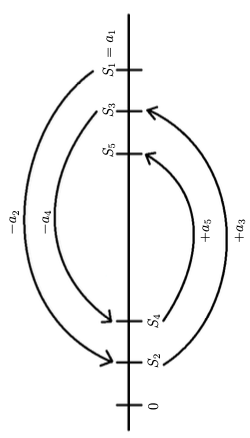
\includegraphics[scale=0.1]{leibniz.png}
  \end{wrapfigure}
  Wenn $(a_n) \ge 0, \forall n \ge 1$ monoton fallend und $\limn a_n = 0$ ist, dann konvergiert $S = \sumk (-1)^{k+1} a_k$ und $a_1 - a_2 \le S \le a_1$. \\
  \tiny \color{gray}
    Monoton fallende Folge alternierend summiert, ist konvergent.
  \normalsize \color{black} 
\end{subbox}

\begin{bspbox}{Beispiel Leibnizkriterium}
  Gegeben: $\sumn (-1)^{k+1}(\sqrt{k+1} - \sqrt{k})$ \\
  $a_n = \sqrt{n+1} - \sqrt{n} = \frac{(\sqrt{k+1} - \sqrt{k})(\sqrt{k+1} + \sqrt{k})}{\sqrt{k+1} + \sqrt{k}} = \frac{1}{\sqrt{n+1} + \sqrt{n}}$ \\
  $\implies a_n$ ist monoton fallend und $\limn a_n = 0$ \\
\end{bspbox}


\subsection{Wurzel- \& Quotientenkriterium}
Prüfe ob Reihe Divergenz oder absolut konvergent. \\
Wurzelkriterium versagt $\implies$ Quotientenkriterium versagt. \\
$\nLeftarrow$ Gibt Bsp. wo Wurzelk. funktioniert \& Quotientenk. nicht.

\subsubsection{Quotientenkriterium}
Prüfen ob absolut Konvergent oder divergent. \\
\begin{mainbox}{Quotientenkriterium (bei $!, \ x^n, \ ...)$}
  Sei $(a_n)_{n \geqslant 1}$ die Folge der Glieder mit $a_n \neq 0$ $\forall n \geqslant 1$
  \begin{equation*}
    \limn \left| \frac{a_{n + 1}}{a_n} \right| =
    \begin{cases}
      < 1, & absolute Konvergenz \\
      = 1, & keine Aussage       \\
      > 1, & Divergenz
    \end{cases}
  \end{equation*}
  \tiny \color{gray}
    Falls Grenwzert unbekannt: \\
    $\limn \sup \left| \frac{a_{n + 1}}{a_n} \right| < 1 \Rightarrow \text{konvergiert absolut}$ \qquad
    $\limn \inf \left| \frac{a_{n + 1}}{a_n} \right| > 1 \Rightarrow \text{divergiert}$ \\
  \normalsize \color{black}
\end{mainbox}

\begin{bspbox}{Beispiel Quotientenkriterium}
  $\sum_{k=1}^{\infty} \frac{n!}{n^n}$ konvergiert. Beweis: \\
  $\limn \left| \frac{a_{n + 1}}{a_n} \right| 
  = \limn \left| \frac{(n+1)!}{(n+1)^{n+1}} \cdot \frac{n^n}{n!} \right| \\
  = \limn \left| \left(\frac{(n+1)!}{n!}\right) \cdot \left(\frac{n}{n+1}\right)^n \cdot \frac{1}{n+1}\right| \\
  = \limn \left| (n+1) \cdot \left(\frac{n}{n+1}\right)^n \cdot \frac{1}{n+1}\right| 
  = \limn \left| \left(\frac{n}{n+1}\right)^n \right| \\
  = \limn \left| \left(\frac{1}{\frac{n+1}{n}} \right)^n \right|
  = \limn \left| \frac{1}{(1 + \frac{1}{n})^n} \right| 
  = \frac{1}{e} < 1$ \\
\end{bspbox}

\subsubsection{Wurzelkriterium}
Prüfen ob absolut Konvergent oder divergent. \\
\begin{mainbox}{Wurzelkriterium (bei $(\cdot)^n, \ x^n, \ !, \ ...$)}
  Sei $(a_n)_{n \geqslant 1}$ die Folge der Glieder  
  \begin{equation*}
    \limn \sqrt[n]{\left| a_n \right|} =
    \begin{cases}
      < 1, & absolute Konvergenz \\
      = 1, & keine Aussage       \\
      > 1, & Divergenz
    \end{cases}
  \end{equation*}
  \tiny \color{gray}
  Falls Grenwzert unbekannt: \\
  $\limn \sup  \sqrt[n]{\left| a_n \right|}  < 1 \Rightarrow \text{konvergiert absolut}$ \qquad
  $\limn \sup  \sqrt[n]{\left| a_n \right|}  > 1 \Rightarrow \text{divergiert}$ \\
\normalsize \color{black}
\end{mainbox}

\begin{bspbox}{Beispiel Wurzelkriterium}
  $\sum_{k=1}^{\infty} \left(\frac{5n + 2n^3}{6n^3 + 5}\right)^n$ 
  $\implies a_n = \left(\frac{5n + 2n3}{6n^3+5}\right)^n$\\
  $\implies |a_n|\frac{1}{n}= \left|\frac{5n + 2n^3}{6n^3 + 5}\right|^n \implies \limn \frac{2}{6}$\\
  $\implies \limn \sqrt[n]{\left| a_n \right|} = \frac{1}{3} < 1 \implies \text{konvergiert absolut}$ \\
\end{bspbox}

\subsection{Doppelreihen Satz}
\begin{subbox}{Doppelreihen Satz (Cauchy)}
  Falls $\exists B > 0$ sodass $\sum_{j= 0}^{m}\sum_{i = 0}^{m} |c_{ij}| \geqslant B \quad \forall m \geqslant 0$.
  Dann ist jede lineare Anordnung der doppelreihe $\sum_{i,j}^{} c_{ij}$ \textit{absolut konvergent} und es gilt: \\
  $\sum_{j= 0}^{\infty} \sum_{i = 0}^{\infty} |c_{ij}| =  \sum_{i = 0}^{\infty} \sum_{j= 0}^{\infty} |c_{ij}|$
\end{subbox}

\subsection{Cauchy-Produkt}
\tiny \color{gray} 
  \textbf{Hinweis}: Cauchy Produkt von 2 divergenten Reihen kann konvergent sein. Dann kann keine Aussage über ihre Konvergenz basiernd auf den Reihen $a_n$ und $b_n$ gemacht werden. 
\normalsize \color{black}
\begin{subbox}{Cauchy-Produkt (Reihen multiplizieren)}
  Das Cauchy-Produkt von zwei Reihen $\sum_{i = 0}^\infty a_i$ und $\sum_{j = 0}^\infty b_j$ ist definiert als: \\
  $\sum_{n=0}^\infty \sum_{j=0}^n (a_{n-j} \cdot b_j) = a_0b_0 + (a_0b_1 + a_1b_0) + \ldots$ \\
  Es konvergiert, falls beide Reihen \textit{absolut} konvergieren. \\
\end{subbox}

\section{Stetige Funktionen}
\subsection{Reelwertige Funktionen}
Sei $D \subseteq \mathbb{R}$ eine beliebige Menge. Eine reelwertige Funktion ist eine Abbildung $f: D \rightarrow \mathbb{R}$.
Die Menge aller auf D definierten Funktionen: $\mathbb{R} = \{f: D \rightarrow \mathbb{R} | f \text{eine Funktion}\}$. \\
$\forall x \in D$: ($\R^D, +, \cdot$) ist ein Vektorraum. \\

\begin{itemize}[leftmargin=4.5mm, topsep=1pt, parsep=1pt]
  \item \textbf{Addition}: $(f+g)(x) = f(x) + g(x)$ \\
  \item \textbf{Skalare Multiplikation}: $(\lambda f)(x) = \lambda \cdot f(x)$
  \item \textbf{Nullfunktion}: $0(x) = 0 \forall x \in D$ \\
  Entspricht Nullvektor in $\mathbb{R}^D$. \\
  \item  \textbf{Produkt von Funktionen}: $(f \cdot g)(x) = f(x) \cdot g(x)$ 
  \item  \textbf{Konstante Funktion}: $(f \cdot 1)(x) = f(x)$ \\
         Entspricht dem Einheitsvektor in $\mathbb{R}^D$. \\
  \item \textbf{Quotient von Funktionen}: Sei $f,g : D \rightarrow \mathbb{R}$ und $\tilde{D} = \{ x \in D | g(x) \neq 0\}$. $(\frac{f}{g})(x) = \frac{f(x)}{g(x)}$ 
  \item \textbf{Komposition: Verkettung von Funktionen}: Zuerst $f$, dann $g$. Sei $f: D \rightarrow \mathbb{R}$ \& $g: E \rightarrow \mathbb{R}$ \\
        $g \circ f: D \rightarrow \mathbb{R}$ mit $(g \circ f)(x) = g(f(x))$.
\end{itemize}


\subsection{Beschränktheit}
$f : D \rightarrow \mathbb{R}$ ist: \\
\begin{itemize}[leftmargin=4.5mm, topsep=1pt, parsep=1pt]
  \item \textbf{nach oben beschränkt}: falls $f(D) \subset \mathbb{R}$ n.o.b. 
  \item \textbf{nach unten beschänkt}: falls $f(D) \subset \mathbb{R}$ n.u.b. 
  \item \textbf{beschränkt}: falls $f(D) \subset \mathbb{R}$ n.o.b \& n.u.b.
\end{itemize}

\subsection{Kompaktes Intervall}
Ist ein Intervall $I \subset \R$ falls $I = [a, b], a \le b$.
\begin{itemize}[leftmargin=4.5mm, topsep=1pt, parsep=1pt]
    \item Für $(x_n)_{n \in \N}, \lim_{n \to \infty}x_n \in \R, a \le b$. \\
          $\{x_n | n \ge 1\} \subset [a, b] \implies \lim_{n \to \infty}x_n \in [a, b]$. \\
          \tiny \color{gray}
            Jede konvergente Folge die immer im Intervall $[a, b]$ liegt, hat ihren Grenzwert in $[a, b]$.
          \normalsize \color{black}
\end{itemize}


\subsection{Monotonie von Funktionen}

\begin{mainbox}{$f$ ist monoton}
$f : D \to \R, D \subset R, \ \forall x,y \in D$ ist:
\begin{itemize}[leftmargin=4.5mm, topsep=1pt, parsep=1pt]
    \item \textbf{monoton wachsend} falls $x \le y \Rightarrow f(x) \le f(y)$.
    \item \textbf{streng mono. wachs.:} falls $x < y \Rightarrow f(x) < f(y)$.
    \item \textbf{monoton fallend:} falls $x \ge y \Rightarrow f(x) \ge f(y)$.
    \item \textbf{streng mon. fallend:} falls $x > y \Rightarrow f(x) > f(y)$.
  \end{itemize}

\end{mainbox}
\begin{itemize}[leftmargin=4.5mm, topsep=1pt, parsep=1pt]
  \item \textbf{monoton:} falls mono. wachsend oder mono. fallend.
  \item \textbf{streng monoton:} falls streng monoton wachsend oder streng monoton fallend.
  \item Symmetrische Funktionen sind nie monoton.
  \item $f$ streng mono. wachsend $\implies$ $f$ injektiv
\end{itemize}


\subsection{Definition Stetigkeit von $f$}
\begin{wrapfigure}{r}{0.1\textwidth} 
  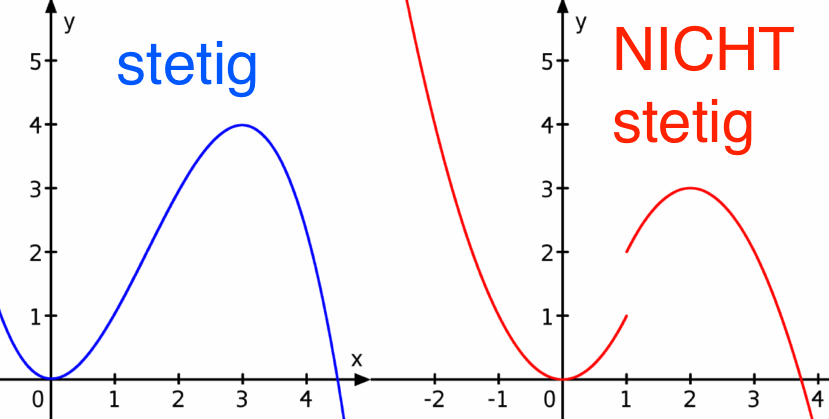
\includegraphics[scale=0.08]{stetignichtstetig.png}
\end{wrapfigure}
Keine sprunghafte Änderungen: \\
Kleine Änderung Argument $\implies$ kleine Änderung Funktionswert. \\
Sei $D \subseteq \mathbb{R}^d$ und $f: D \rightarrow \mathbb{R}^d, \, x \rightarrow f(x)$ eine Funktion. \\

\begin{mainbox}{$f$ Stetig in $x_0$ (Punktweise) (\epsilon-Kriterium)}
  \begin{wrapfigure}{r}{0.13\textwidth} 
    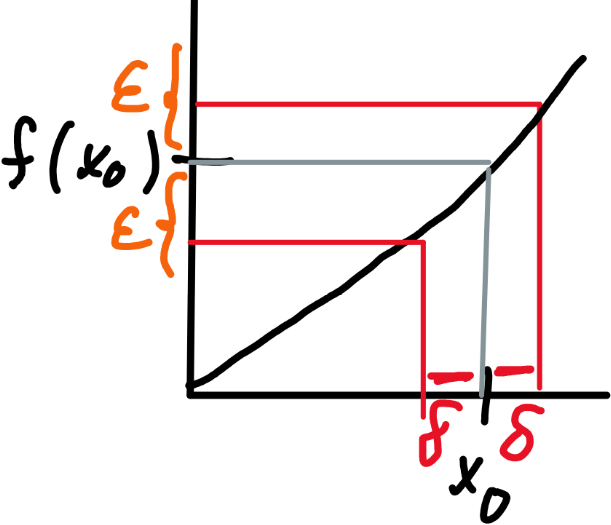
\includegraphics[scale=0.07]{punktweise_stetigkeit.jpeg}
  \end{wrapfigure}
  Funktion $f$ stetig in $x_0 \in D$ falls: \\
  $\forall x_0, \ \forall \epsilon > 0, \ \exists \delta > 0, \ \forall x: $ \\
  $|x-x_0| < \delta \implies |f(x)-f(x_0)| < \epsilon$.
\end{mainbox}

\begin{mainbox}{$f$ stetig in $x_o$ (Punktweise) (Folgenkriterium)}
  \begin{itemize}[leftmargin=4.5mm, topsep=1pt, parsep=1pt]
    \item  $f$ stetig in $x_0$ $\iff (\quad \forall (a_n)_{n \in \N}$ in $D:$ \\ 
          \qquad \qquad $\lim_{n \to \infty} a_n = x_0 \implies \lim_{n \to \infty} f(a_n) = f(x_0))$. \\
          \tiny \color{gray} 
          $f$ stetig in $x_0 \Leftrightarrow \forall$ Folge $(a_n)$ konv. gegen $x_0$, Bildfolge $f(a_n)$ konv. gegen $f(x_0)$.
          \normalsize \color{black}
    \item $f$ stetig in $x_0 \iff \forall (a_n)_{n \in \N}$ in $D$: \\
          \qquad \qquad \qquad \qquad $\lim_{n \to \infty} f(a_n) = f( \lim_{n \to \infty} a_n)$ \\
            \tiny \color{gray}
              Anwendung Operation "Funktion" \& "Grenzwert" können vertauscht werden.
            \normalsize \color{black}
  \end{itemize}
\end{mainbox}

\begin{mainbox}{$f$ Stetig}
  $f$ ist für alle $x_0 \in D$ Punktweise stetig. \\
\end{mainbox}
\begin{itemize}[leftmargin=4.5mm, topsep=1pt, parsep=1pt]
  \item Für nicht-kompaktes Intervall $D = \ ]a,b[$ \ :  \\
        Punktweise stetig $\implies$ stetig im Intervall.
  \item Für kompaktes Intervall $D = \ [a,b]$ \ : \\
        Punktweise stetig + Beweis stetig in Randpunkten $\implies$ stetig im Intervall. 
        \tiny \color{gray}
            Für die Randpunkte zeigen dass $lim_{x \to a^+} f(x) = f(a)$ und $lim_{x \to b^-} f(x) = f(b)$.
        \normalsize \color{black}
  \item $f$ stetig $\notimplies f$ differenzierbar
  \item $f$ stetig auf \textit{kompaktem intervall} $\implies f$ beschränkt
\end{itemize}


\begin{mainbox}{$f$ Gleichmässig Stetig}
  Stärkere Form der Stetigkeit. $\forall$ Punktepaare im Definitionsbereich der Funktion existiert gemeinsames $\delta$. \\ 
  $\forall \epsilon > 0, \exists \delta > 0, \forall x, y \in D:$ \\
  $|x-y| < \delta \implies |f(x)-f(y)| < \epsilon$
\end{mainbox}
\begin{itemize}[leftmargin=4.5mm, topsep=1pt, parsep=1pt]
  \item gleichmässig stetig $\implies$ stetig $\implies$ in $x_0$ stetig
  \item $f: [a, b] \to \R$ stetig im Kompakten Intervall $\implies f$ ist in $[a,b]$ gleichmässig stetig.
\end{itemize}

\subsubsection{Polynomiale Funktionen}
Polynomiale Funktionen $P(x)$ sind auf ganz $\R$ stetig. \\
$P(x) = a_n x^n + a_{n-1} x^{n-1} + \ldots + a_1 x + a_0$ \\

\subsubsection{Rechenregeln Stetige Funktionen}
  Für $x_0 \in D \subset \R, \lambda \in \R, f: D \to \R, g: D \to \R$ und \\
    $f$ und $g$ stetig in $x_0$
  \begin{itemize}[leftmargin=7mm, topsep=1pt, parsep=1pt] 
    \item[$\Rightarrow$] $f + g, f + (-g), \lambda \cdot f, f \cdot g$ stetig in $x_0$.
    \item[$\Rightarrow$] $\frac{f}{g}: D' \to \R, x \mapsto \frac{f(x)}{g(x)}, \ D' = \{x \in D | g(x) \neq 0\}, g(x_0) \neq 0$, ist stetig in $x_0$.
\end{itemize}

Für $D_1, D_2 \subset \R, f: D_1 \to D_2, g: D_2 \to \R, x_0 \in D_1$:
\begin{itemize}[leftmargin=4.5mm, topsep=1pt, parsep=1pt] 
    \item Falls $f$ in $x_0$ und $g$ in $f(x_0)$ stetig $\implies g \circ f : D_1 \to \R$ ist in $x_0$ stetig.
    \item Falls $f$ auf $D_1$ und $g$ auf $D_2$ stetig $\implies g \circ f$ auf $D_1$ stetig.
\end{itemize}

Für $D \subset \R, f, g: D \to \R, x_0 \in D$. 
\begin{itemize}[leftmargin=4.5mm, topsep=1pt, parsep=1pt] 
  \item Falls $f, g$ stetige Funktionen $\implies |f|, (max\{f,g\}),$ \\
            $(min\{f,g\})$ stetig in $x_0$. \\
              \tiny \color{gray}
            Bsp: $(max\{f,g\})(x) = max\{f(x), g(x)\} \forall x \in D$
            \normalsize \color{black}
\end{itemize}

\subsection{Zwischenwertsatz}
\tiny \color{gray}
  Anwendung: Zeigen, das eine Funktion einen gewissen Wert annimmt. \\
  Anwendung: Zeigt, dass eine Funktion $f$ jeden Wert zwischen $f(a)$ und $f(b)$ annimmt. \\
\normalsize \color{black}
\begin{mainbox}{Zwischenwertsatz}
  Intervall $I \subseteq \R$ \& stetige Funktion $f: I \to \R$ \& $a, b \in I$ $\implies \forall y$ sodass $f(a) \leqslant y \leqslant f(b)$ existiert $c$ \\
  \qquad sodass $a \le c \le b$ mit $y = f(c)$. \\
\end{mainbox}
\begin{itemize}[leftmargin=4.5mm, topsep=1pt, parsep=1pt] 
  \item Daraus folgt, dass ein Polynom mit ungeradem Grad mindestens eine Nullstelle in $\R$ besitzt.
  \item Nullstellenmove: stetige Funktion $f$ an einem Punkt kleiner und einem Punkt grösser als 0 $\implies f(x) = 0$ an mindestens einem Punkt.
  \item $x, y \in R, x \le y$, $c$ liegt \textbf{zwischen} $x$ und $y$ falls $c \in [x, y]$.
  \item Für $f: [a,b] \to \R$ stetig und $f(a) \cdot f(b) < 0 \implies \exists c \in ]a,b[: f(c) = 0$.
\end{itemize}

\begin{bspbox}{Beispiel Zwischenwertsatz (Nullstellenmove)}
  \tiny \color{gray}
    Hilfsfunktion \& Nullstellenmove zeigen dass stetige Funktion $f$ Wert $e^x$ annimmt. \\
  \normalsize \color{black}
  \textit{Zu beweisen:} Wenn $f(0) < 1$ \& $f(1) > 1$, dann $\exists x \in [0,1]$ s.t. $f(x) = e^x$. \\
  \textit{Proof:} Define Hilfsfunktion $g(x) = f(x) - e^x$. \\
  $g(x)$ ist stetig weil Differenz von stetigen Funktionen ist stetig. Erfüllt $g(0) < 0$ \& $g(1) > 0$. \\
  $\Rightarrow \exists$ s.t. $g(x) = 0 \Rightarrow g(x) = f(x) - e = 0 \Rightarrow f(x) = e^x$. \\
\end{bspbox}

\subsection{Min-Max-Satz}
\tiny \color{gray}
Anw.: kompaktes Intervall \& $f$ stetig $\implies$ Bild $f(x)$ beschränkt. \\
Anw.: kompaktes Intervall \& $f$ stetig $\implies$ Bild hat min/max \& $\inf f(x)/\sup f(x)$. 
\normalsize \color{black} \\
\begin{mainbox}{Min-Max-Satz}
  Sei $f: I = [a,b] \to \R$ stetig auf kompaktem Intervall $I$. \\
  $\implies \exists u, v \in I$ mit $f(u) \le f(x) \le f(v), \ \forall x \in I$. \\
  $\iff f([a, b])$ ist beschränkt. $f([a, b]) \subset [f(u), f(v)]$
  \begin{itemize}
    \item[$\implies$] $\exists minimum \implies f(u) = inf\{f(x) | x \in I\}$
    \item[$\implies$] $\exists maximum \implies f(v) = sup\{f(x) | x \in I\}$
  \end{itemize}
\end{mainbox}

\subsection{Umkehrabbildung}
Sei $f: I \rightarrow \mathbb{R}$ stetig und streng monoton. Dann ist $f^{-1} : J \rightarrow I$ stetig und streng monoton wobei $J = f(I) \subset \mathbb{R}$.
\tiny \color{gray}
  Wenn $f$ stetig, dann Umkehrfunktion $f^{-1}$ stetig. \\
  Wenn $f$ streng monoton, dann Umkehrfunktion $f^{-1}$ streng monoton. \\
\normalsize \color{black}

\subsection{Exponentialfunktion Rechenregeln}
\begin{wrapfigure}{r}{0.05\textwidth} 
  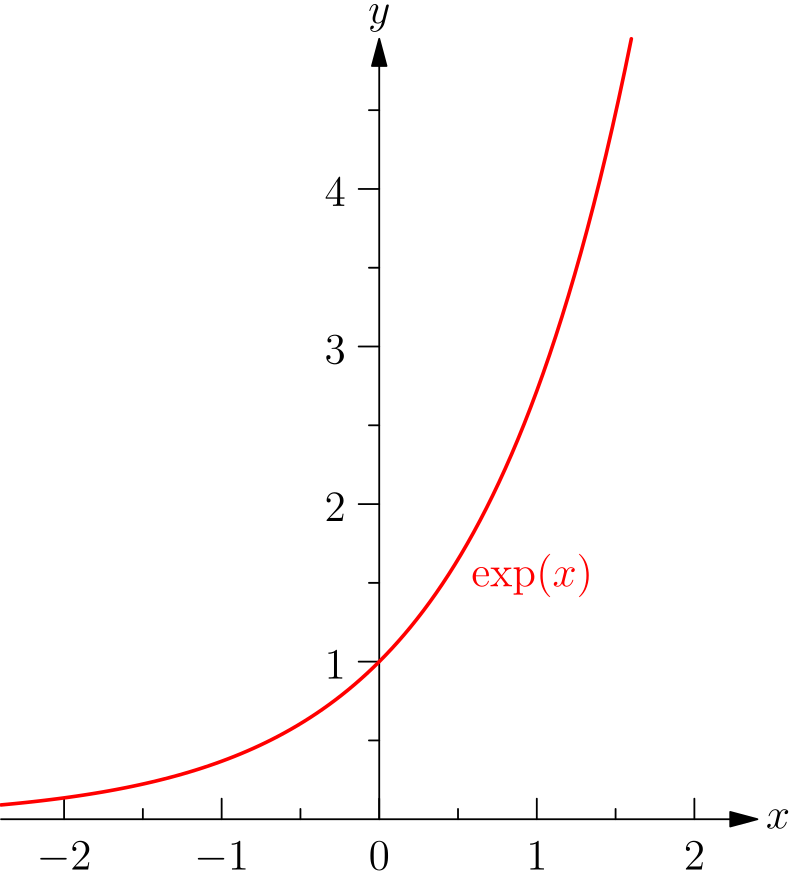
\includegraphics[scale=0.05]{exponentialfunktion.png}
\end{wrapfigure}
Exponentialfunktion $\exp: R \to ]0, +\infty[$. \\
$f(x) = exp(x) \Leftrightarrow f(x) = e^x \Leftrightarrow \sumk \frac{x^k}{k!}$ \\
$exp$ ist: 
\begin{inparaitem}
  \item streng mon. wachsend
  \item stetig
  \item surjektiv ($\Rightarrow$ bijektiv)
\end{inparaitem}

\begin{inparaitem}
  \item $\exp(x) = 1 + x + \frac{x^2}{2!} + \dots \ge 1$ \\
  \item $\exp(x + y ) = \exp(x) \cdot \exp(y) \ \forall x,y \in \C$ \\
  \item $\exp(x - y ) = \frac{\exp(x)}{\exp(y)} \ \forall x,y \in \C$ \\
  \item $\exp(0) = 1$  \qquad \qquad   \qquad \quad    \item $\exp(1) = e$ \\
  \item $\exp(x) > 0  \forall x \in \R$ \qquad \qquad  \item $\exp(x) > 1 \ \forall x > 0$ \\
  \item $\exp(x) > \exp(y) \ \forall x > y$ \qquad     \item $\exp(x) > 1 + x \ \exists x \in \R$
\end{inparaitem}

\subsection{Natürlicher Logarithmus}
\begin{wrapfigure}{r}{0.05\textwidth} 
  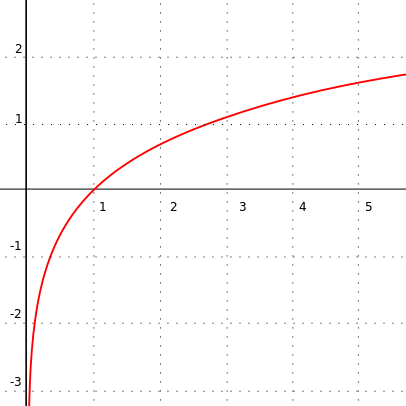
\includegraphics[scale=0.1]{lnfunktion.png}
\end{wrapfigure}
Umkehrabbildung von $\exp$ ist $\ln: \ ]0, +\infty[ \to \R$ \\
$\ln(x)$ ist:
  \begin{inparaitem}
    \item streng mon. wachsend
    \item stetig
    \item bijektiv
  \end{inparaitem}

\begin{itemize}[leftmargin=4.5mm, topsep=1pt, parsep=1pt]
    \item \begin{inparaitem}
        \item $\ln(1) = 0$
        \item $\ln(e) = 1$
      \end{inparaitem}
    \item $\ln(exp(x)) = x \ \forall x \in \R$
    \item $\ln(a \cdot b) = \ln(a) + \ln(b) \ \forall a,b \in ]0, +\infty[$
\end{itemize}

\subsection{Potenzfunktionen Rechenregeln }
\begin{wrapfigure}{r}{0.03\textwidth} 
  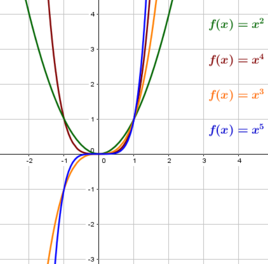
\includegraphics[scale=0.18]{potenzfunktion.png}
\end{wrapfigure}
Potenzfunktion: $f(x) = x^n$
  \tiny \color{gray}
    Bsp: $f(x) = x^2$, $f(x) = x^3$, etc. \\
  \normalsize \color{black}
  Für $x > 0, a \in \R \ x^a := \exp(a \ln(x))$
\begin{itemize}[leftmargin=4.5mm, topsep=1pt, parsep=1pt]
    \item Für $a > 0$ ist $x \mapsto x^a$ \\
      \qquad \begin{inparaitem}
        \item streng monoton wachsend
        \item stetig
        \item bijektiv
      \end{inparaitem}
    \item Für $a < 0$ ist $x \mapsto x^a$ \\
      \qquad \begin{inparaitem}
          \item streng monoton fallend
          \item stetig
          \item bijektiv
        \end{inparaitem}
    \item $\ln(x^a) = a \ln(x) \ \forall a \in R, \ \forall x > 0$
    \item $x^a \cdot x ^b = x^{a + b} \ \forall a,b \in R, \ \forall x > 0$
    \item $(x^a)^b = x^{a \cdot b} \ \forall a,b \in R, \ \forall x > 0$
\end{itemize}

\subsection{Konvergenz der Funktionenfolge}
Sei \textbf{Funktionenfolge} $(f_n)_{n \geqslant 1}$ Abbildung $\N \mapsto \{ f: D \rightarrow \R \}$ \\
    \qquad $(f_n)_{n \geqslant 1} = \{f_1, f_2, ..., f_n\}$ \\
Sei $f_n$ eine der Funktionen für ein $n$, also die Abbildung: $n \mapsto f_n : D \rightarrow \R$  
  \tiny \color{gray}
    Beispiel: $f_n(x) = nx$: $f_1(x) = x, f_2(x) = 2x$, etc. \\
  \normalsize \color{black}
Sei $f(x) = \limn f_n(x)$ die \textbf{Grenzwertfunktion} von $(f_n)$. Sie gibt für jedes $x$ den Grenzwert der Funktionenfolge an. \\

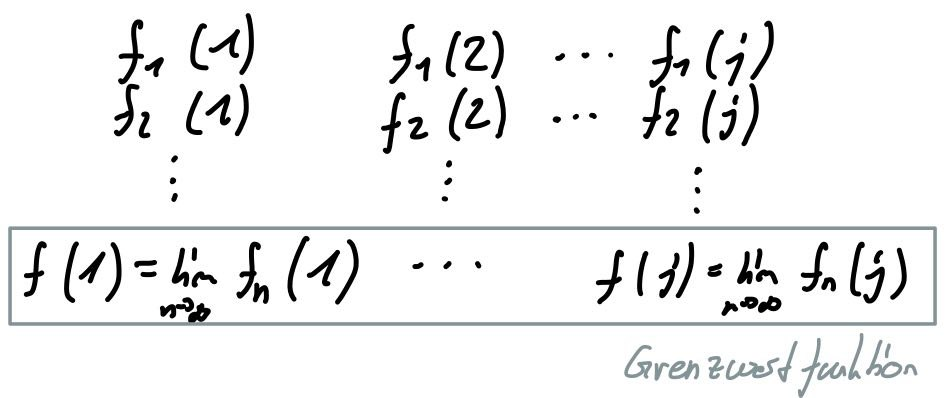
\includegraphics[scale=0.09]{funktionenfolgenundgrenzwertfunktion.jpg}
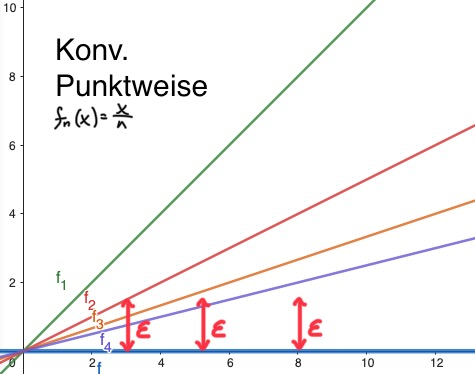
\includegraphics[scale=0.15]{konvpunktweise_nicht_gleichmaessig.jpg}
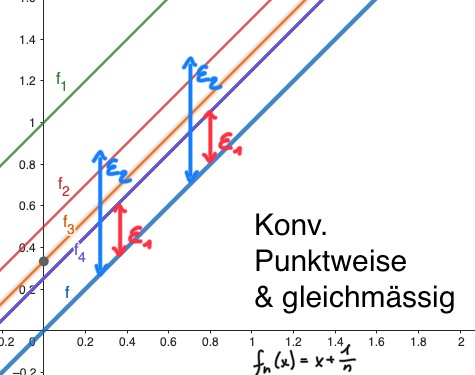
\includegraphics[scale=0.15]{konvpunktweise_und_gleichmaessig.jpg}


\begin{mainbox}{$(f_n)_{n \geqslant 1}$ konvergiert punktweise (\epsilon-Kriterium)}
  Funktionenfolge $(f_n)_{n \geqslant 1}$ konvergiert punktweise gegen Funktion $f: D \to \R \iff$  \\
  $\forall x \in D, \forall \epsilon > 0, \exists N \in \N s.t. \forall n \geqslant N: |f_n(x) - f(x)| < \epsilon$.
  \tiny \color{gray}
    Konv. punktweise $\iff$ Für jedes x gibt es ein Ausnahmeindizes N nach welchem die Funktionswerte aller folgenden Funktionen $f_n(x)$ in einer $\epsilon$-Umgebung der Grenzfunktion $f(x)$ liegen.
  \normalsize \color{black}
\end{mainbox}

\begin{mainbox}{$(f_n)_{n \geqslant 1}$ konvergiert punktweise (Folgenkriterium)}
Funktionenfolge $(f_n)_{n \geqslant 1}$ konvergiert punktweise gegen Funktion $f: D \to \R \iff  \forall x \in D: f(x) = \limn f_n(x)$. \\
\tiny \color{gray}
  Konv. punktweise $\iff$ Für jedes $x$ konvergiert die Funktionenfolge $f_n(x)$ gegen die Grenzfunktion $f(x)$. 
\normalsize \color{black}
\end{mainbox}
\tiny \color{gray}
  Beispiel: Sei $f_n(x) = \frac{x}{n}$ und Grenzfunktion $f(x) = 0$\\
  $x = 3: f_1(3)= \frac{3}{1}, f_2(3) = \frac{3}{2}, f_3(3) = \frac{3}{3}, f_4(4) = \frac{3}{4},...$ \qquad $f(3) = 0$ \\
  $x = 4: f_1(4)= \frac{4}{1}, f_2(4) = \frac{4}{2}, f_3(4) = \frac{4}{3}, f_4(4) = \frac{4}{4},...$ \qquad $f(4) = 0$ \\
  $x = 5: f_1(5)= \frac{5}{1}, f_2(5) = \frac{5}{2}, f_3(5) = \frac{5}{3}, f_4(5) = \frac{5}{4},...$ \qquad $f(5) = 0$ \\
\normalsize \color{black}

\begin{mainbox}{$(f_n)_{n \geqslant 1}$ konvergiert gleichmässig}
  Funktionenfolge $(f_n)_{n \geqslant 1}$ konvergiert gleichmässig gegen Funktion $f: D \to \R \iff \forall \epsilon > 0 \ \exists N \ge 1$,  \\ 
   s.t. $\forall n \ge N, \ \forall x \in D: | f_n(x) - f(x) | \le \epsilon$. \\
   \tiny \color{gray}
      Konv. gleichmässig $\iff$ Es gibt ein Ausnahmeindizes N nach welchem die Funktionswerte aller folgenden Funktionen $f_n(x)$ für jedes $x$ in derselben $\epsilon$-Umgebung der Grenzfunktion $f(x)$ liegen.
      $\iff$ Für jedes x konvergiert die Funktionenfolge $f_n(x)$ \textit{gleich schnell} gegen die Grenzfunktion $f(x)$. 
    \normalsize \color{black}
\end{mainbox}
\tiny \color{gray}
  Beispiel: Sei $f_n(x) = x + \frac{1}{n}$ und Grenzfunktion $f(x) = x$\\
  $x = 3: f_1(3)= 3 + \frac{1}{1}, f_2(3) = 3 + \frac{1}{2}, f_3(3) = 3 + \frac{1}{3}, f_4(3) = 3 + \frac{1}{4},...$ \qquad $f(3) = 3$ \\
  $x = 4: f_1(4)= 4 + \frac{1}{1}, f_2(4) = 4 + \frac{1}{2}, f_3(4) = 4 + \frac{1}{3}, f_4(4) = 4 + \frac{1}{4},...$ \qquad $f(4) = 4$ \\
  $x = 5: f_1(5)= 5 + \frac{1}{1}, f_2(5) = 5 + \frac{1}{2}, f_3(5) = 5 + \frac{1}{3}, f_4(5) = 5 + \frac{1}{4},...$ \qquad $f(5) = 5$ \\
\normalsize \color{black}

\begin{itemize}[leftmargin=4.5mm, topsep=1pt, parsep=1pt] 
  \item Für $\mathbb{D} \subset \R$ und Funktionenfolge $f_n:\mathbb{D} \to \R$ bestehend aus in $\mathbb{D}$ stetigen Funktionen die gleichmässig gegen Funktion $f: \mathbb{D} \to \R$ konvergieren $\implies f$ ist in $\mathbb{D}$ stetig.
  \item Falls $f_n$ gleichmässig zu $f$ konvergiert \\
          \qquad $\implies \limsup_{n \to \infty} \left| f_n(x) - f(x) \right| = 0, x \in \mathbb{D}$.
  \item $(f_n)$ konv. gleichmässig gegen $f(x) \implies f(x)$ ist stetig
  \item $(f_n)$ konv. gleichmässig gegen $f(x) \notimplies f(x)$ ist differenzierbar
\end{itemize}

\begin{mainbox}{$(f_n)_{n \geqslant 1}$ gleichmässig konvergent}
  Funktionenfolge $(f_n)_{n \geqslant 1}$ gleichmässig konvergent, falls: 
  \begin{itemize}[leftmargin=4.5mm, topsep=1pt, parsep=1pt]
    \item $\forall x\in D$ existiert Grenzwert $\limn f_n(x) = f(x)$
    \item und $(f_n)_{n \geqslant 1}$ gleichmässig gegen $f$ konvergiert.
  \end{itemize}
\end{mainbox}


\begin{subbox}{Cauchy Kriterium für Gleichmässige Konvergenz}
  $f_n : \mathbb{D} \to \R$ ist gleichmässig konvergent $\iff \forall \epsilon > 0 \ \exists N \ge 1: \ \forall n,m \ge N \ \forall x \in D: \left| f_n(x) - f_m(x) \right| < \epsilon$.
\end{subbox}

\begin{itemize}[leftmargin=4.5mm, topsep=1pt, parsep=1pt]
  \item Falls $f_n:\mathbb{D} \to \R$ gleichmässig konvergente Folge stetiger Funktionen $\implies f(x) := \lim_{n \to \infty} f_n(x)$ stetig.
  \item Alle $f_n$ stetig und $f_n \to f \implies f$ ist stetig.
  \item $(f_n)_{n \geq 1}$ und $(f')_{n \geq 1}$ gleichmässig in $]a, b[$ konvergent mit $\limn f_n = f$ und $\limn f'_n = p \implies f$ stetig differenzierbar und $f' = p$.
\end{itemize}


\begin{bspbox}{Punktweise vs. gleichmässige Konvergenz}
  Sei $f_n(x) = \frac{x}{n}$ eine Funktionenfolge.

  \textbf{Punktweise konvergenz} \\
  Sei $x \in [0,\infty) \Rightarrow$ konv. punktweise gegen $f(x) = 0$. \\ 
  
  \textit{Nicht gleichmässig konv.} weil wenn $x$ grösser wird, konv. Funktion langsamer gegen 0.
  
  \textbf{Gleichmässig konvergent} \\
  Sei $x \in [0, 1] \Rightarrow$ konv. gleichmässig gegen $f(x) = 0$. \\
  
  Bei gleichmässiger Konvergenz hängt die Konvergenzgeschwindigkeit nicht von $x$ ab. 
  Da $x$ maximal $1$ ist, hat es keinen Einfluss auf die Konvergenzgeschwindigkeit. \\
  Sei $N > \frac{1}{\epsilon}$, dann gilt $\forall n \geq N, \forall x \in [0,1]:$ \\  
  $f_n(x)-f(x) = \frac{x}{n} \leq \frac{1}{n} \leq \frac{1}{N} < \epsilon$ 
\end{bspbox}

\begin{bspbox}{Konvergenz von Funktionenfolgen}
  \textbf{1. $f(x)$ finden durch punktweiser Limes von $f_n$} \\
  Punktw. Limes von $f_n$ auf Definitionsbereich $\Omega$ finden. Für fixes, beliebiges $x$ ($n$ ist Variable): $\lim_{n \rightarrow \infty} f_n(x) = f(x)$. \\
  \textbf{2. $f$ konvergiert gleichmässig prüfen} \\
  \textbf{A)} Indirekte Methode:\\
  \begin{itemize}[leftmargin=4.5mm, topsep=1pt, parsep=1pt]
    \setlength\itemsep{0em}
    \item $f$ unstetig $\Rightarrow$ keine gleichmässige Konvergenz
    \item $f$ stetig, monoton wachsend \\ ($f_n(x) \leq f_{n+1}, \ \forall x \in \Omega$) und \\ $\Omega$ kompakt $\Rightarrow$ gleichmässige Konvergenz
  \end{itemize}
  \textbf{B)} Direkte Methode:\\
  \begin{enumerate}[leftmargin=4.5mm, topsep=1pt, parsep=1pt]
    \setlength\itemsep{0em}
    \item Berechne $\sup_{x \in \Omega} |f_n(x)-f(x)|$ (entweder man sieht Maximum direkt oder man rechnet die Ableitung von $|f_n(x)-f(x)|$ und setzt sie gleich 0).
    \item Limes für $n \rightarrow \infty$ von $\sup_{x \in \Omega} |f_n(x)-f(x)|$ berechnen. Wenn Limes $= 0 \Rightarrow f_n$ auf $\Omega$ gleichmässig konvergent.
  \end{enumerate}
\end{bspbox}


\begin{bspbox}{Beweis Gleichmässig Konvergent}
Sei $D = [0, 1]$ und $f_n(x) = \frac{x}{n^2} + x + 1$. \\
\begin{itemize}[leftmargin=4.5mm, topsep=1pt, parsep=1pt]
  \item[1.] Grenzfunktion $f(x)$ finden durch punktweisen limes \\
            \quad $\limn(\frac{x}{n^2} + x + 1) = lim(\frac{x}{n^2}) + x + 1 = x + 1$ \\
  \item[2.] Gleichmässige konvergenz zeigen:  $|f_n(x) - f(x)|$ \\
            $ = |\frac{x}{n^2} + x + 1 - (x + 1)| = |\frac{x}{n^2}| = \frac{x}{n^2} \leq \frac{1}{n^2} \leq \frac{1}{N^2} < \epsilon$.
\end{itemize}
\end{bspbox}


\subsection{Reihe der Funktionenfolge}
\textbf{Reihe der Funktionenfolge} $\sum_{k=0}^{\infty} f_k(x)$ ist unendliche Summe der Funktionenfolge $(f_n)_{n \geqslant 1}$.
\begin{mainbox}{$\sum_{k=0}^{\infty} f_k(x)$ konvergiert gleichmässig}
  Funktionenfolge Ihrer Partialsummen $S_n(x) := \sum_{k=0}^{n} f_k(x)$ konvergiert gleichmässig \\
  $\implies$ Reihe $\sum_{k=0}^{\infty} f_k(x)$ konvergiert gleichmässig
\end{mainbox}
\begin{itemize}[leftmargin=4.5mm, topsep=1pt, parsep=1pt]
  \item Für $\mathbb{D} \subset \R$, Folge stetiger Funktionen $f_n:\mathbb{D} \to \R$. \\
  Falls $\left| f_n(x) \right| \le c_n \ \forall x \in D$ und $\sum_{n=0}^{\infty} c_n$ konvergent \\
  $\implies \sum_{n=0}^{\infty} f_n(x)$ gleichmässig konvergent in $\mathbb{D}$ und Grenzwert $f(x) := \sum_{n=0}^{\infty} f_n(x)$ ist in $\mathbb{D}$ stetig.
\end{itemize}

\subsection{Potenzreihen}
\begin{subbox}{Potenzreihe}
  Die Potenzreihe $\sum_{n=0}^\infty a_n x^n$ mit Entwicklungspunkt $x_0$ ist als $\sum_{n=0}^\infty a_n(x-x_0)^n$ definiert.
\end{subbox}

\begin{itemize}[leftmargin=4.5mm, topsep=1pt, parsep=1pt]
  \item Folge der Partialsummen $S_n(x)$ ist Funktionenfolge. 
  \item Folge der Partialsummen $S_n(x)$ einer Potenzreihe ist definiert als: $S_n(x) = \sum_{k=0}^{n} c_kx^k$.
  \item Potenzreihe $\sum_{n=0}^\infty a_n x^n$ konv. gleichmässig $\implies$ Folge der Partialsummen $S_n(x)$ konv. gleichmässig
\end{itemize}


\begin{mainbox}{$\sum_{n=0}^\infty a_n x^n$ Konvergenzradius um $x_0$}
  \begin{wrapfigure}{r}{0.16\textwidth} 
    \centering
    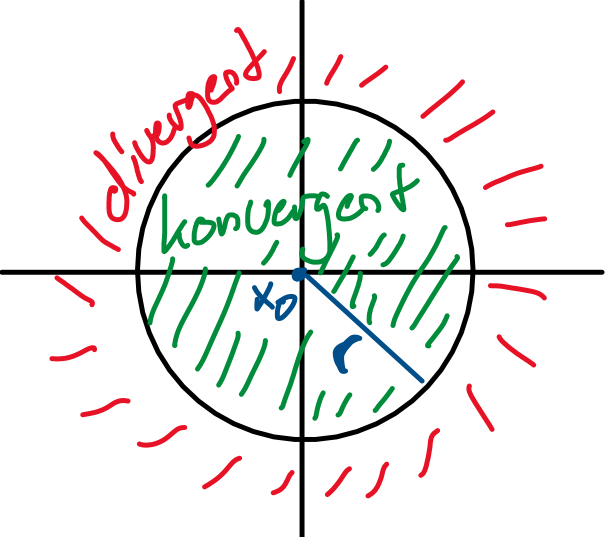
\includegraphics[scale=0.1 ]{konvergenzradius.jpeg}
  \end{wrapfigure}
  Konvergenzradius der Potenzreihe $\sum_{n=0}^\infty a_n x^n$ um Entwicklungspunkt $x_0$ ist grösste Zahl $r$, s.t. die Potenzreihe $\forall x$ mit $|x - x_0| < r$ konvergiert. Falls die Reihe für alle $x$ konvergiert, ist der Konvergenzradius $r$ unendlich. Sonst:
  $$r = \limn \left| \frac{a_n}{a_{n+1}} \right| = \frac{1}{\limn\sup \sqrt[n]{|a_n|}} $$
  \textit{Hinweis:} Konv.rad. hängt nur von $a_n$ ab, nicht von $x^n$.
  \textit{Hinweis:} Konvergenzverhalten jedes Randpunkts $|x - x_0| = r$ muss einzeln untersucht werden.
\end{mainbox}
\tiny \color{gray}
  Sei Potenzreihe: $\sumn \frac{x^k}{k^2}.$ Dann $r = \frac{1}{\limsup \sqrt[n]{a_n}} = \frac{1}{\limsup \sqrt[k]{\frac{1}{k^2}}} = \frac{1}{\limsup \frac{1}{\sqrt[k]{k^2}}} = \frac{1}{\frac{1}{1}} = 1$
\normalsize \color{black}
\begin{itemize}[leftmargin=4.5mm, topsep=1pt, parsep=1pt]
  \item Für Potenzreihe mit positiven Konvergenzradius $\rho > 0$ und $f(x):= \sum_{n=1}^{\infty} c_kx^k, |x| < \rho \implies \forall 0 \le r < \rho$ konvergiert $\sum_{k=0}^{\infty} c_kx^k$ gleichmässig auf $[-r, r]$ und $f:]-\rho, \rho[ \to \R$ ist stetig.
  \item Sind stetig im Innern ihres Konvergenzbereichs
\end{itemize}

\subsection{Grenzwert von Funktionenfolgen}
\subsubsection{Häufungspunkt und Grenzwert}
\begin{mainbox}{$x_0$ ist Häufungspunkt}
  $x_0 \in \mathbb{R}$ ist ein Häufungspunkt der Menge $D$ falls \\
  $\forall \delta > 0 : (]x_0 - \delta, x_0 + \delta[ \ \setminus \{x_0\}) \cap D \neq \emptyset$.
  \tiny \color{gray}
    $x_0$ ist Häufungspunkt, wenn sich in jeder Umgebung von $x_0$ mindestens ein Punkt aus $D$ befindet. \\
  \normalsize \color{black}
\end{mainbox}
\tiny \color{gray}\
  \begin{wrapfigure}{r}{0.08\textwidth} 
    \centering
    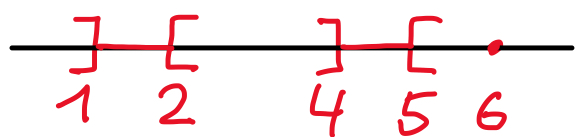
\includegraphics[scale=0.1]{haeufungspunkt.jpeg}
  \end{wrapfigure}
  Bsp: $D = ]1,2[ \cup ]4,5[ \cup \{6\}$, Häufungspunkte: $D' = [1,2] \cup [4,5]$ \\
  \qquad Nicht Häufungspunkt: $6$ weil $x_0 = 6, \delta = \frac{1}{2}$ \\
  \qquad \qquad \qquad \qquad \qquad \qquad $\Rightarrow ([5.5, 6.5] \setminus \{6\}) \cap D = \emptyset$
\normalsize \color{black}

\begin{mainbox}{Grenzwert in Häufungspunkt $x_0$ (\epsilon-Kriterium)}
  \begin{wrapfigure}{r}{0.1\textwidth} 
    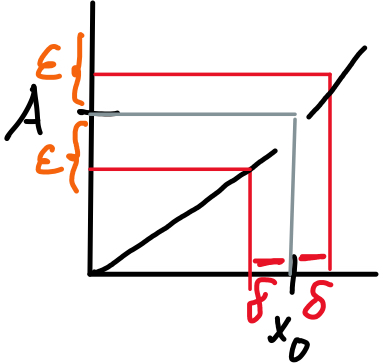
\includegraphics[scale=0.08]{grenzwerthäufungspunkt.jpeg}
  \end{wrapfigure}
  Sei $x_0$ Häufungspunkt von $D$ und $f:D \rightarrow \mathbb{R}$: \\
  $A = \lim_{x \rightarrow x_0} f(x) \iff \forall \epsilon > 0, \ \exists \delta > 0$ s.t. \\
  $\forall x \in D \cap (]x_0-\delta, x_0 + \delta[ \ \setminus \{x_0\}) : |f(x)-A| < \epsilon$.
\end{mainbox}
\scriptsize \color{gray}\
  \begin{wrapfigure}{r}{0.05\textwidth} 
    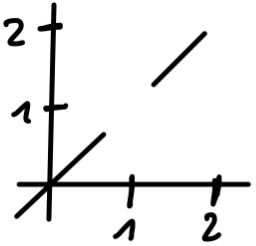
\includegraphics[scale=0.1]{funktionenfolge_grenzwert.jpeg}
  \end{wrapfigure}
  Bsp: \\ 
  Grenzwert existiert, aber f nicht stetig in $x_0 = 1$. \\
  Sei $f: \R\setminus \{]0.8,1.2[\}$. \\
  Grenzwert ungleich Funktionswert: $\lim_{x \to 1} f = 1 \not= f(1)$ 
\normalsize \color{black}

\begin{mainbox}{Grenzwert in Häufungspunkt $x_0$ (Folgenkriterium)}
Sei $x_0$ Häufungspunkt von $D$ und $f:D \rightarrow \mathbb{R}$:  \\
$A = \lim_{n \to x_0}f(x) \iff \forall (a_n)_{n \ge 1} \in \mathbb{D} \setminus \{x_0\}$ mit $\lim_{n \to \infty} a_n = x_0$ folgt $\lim_{n \to \infty}f(a_n) = A$.
\tiny \color{gray}
  Für jede Folge mit Grenzwert $x_0$ ist Grenwzert der Bildfolge $A = \lim_{x \to x_0} f(x)$.
\normalsize \color{black}
\end{mainbox}
\begin{itemize}[leftmargin=4.5mm, topsep=1pt, parsep=1pt]
  \item $f$ muss am Grenzwert $x_0$ nicht zwingend definiert sein.
  \item $f$ ist stetig in $x_0 \in \mathbb{D} \iff \lim_{n \to x_0} f(x) = f(x_0)$.
\end{itemize}

\subsection{Rechenregeln Funktionenfolgen}
\begin{itemize}[leftmargin=4.5mm, topsep=1pt, parsep=1pt]
  \item Für $f,g: \mathbb{D} \to \R$ und falls $\exists \lim_{n \to \infty} f(x)$ und $\lim_{n \to \infty} g(x)$
      \begin{itemize}[leftmargin=9mm, topsep=1pt, parsep=1pt]
          \item[$\implies$] $\lim_{n \to \infty} (f + g)(x) = \lim_{n \to \infty} f(x) + \lim_{n \to \infty} g(x)$
          \item[$\implies$] $\lim_{n \to \infty} (f \cdot g)(x) = \lim_{n \to \infty} f(x) \cdot \lim_{n \to \infty} g(x)$
      \end{itemize}
  \item Für $f,g: \mathbb{D} \to \R, f \le g$ und beide Grenzwerte existieren $\implies \lim_{n \to \infty} f(x) \le \lim_{n \to \infty} g(x)$.
  \item Für $f,g_1, g_2: \mathbb{D} \to \R$, falls $g_1 \le f \le g_2$ und $\lim_{n \to \infty} g_1(x) = \lim_{n \to \infty} g_2(x) \implies \exists \lim_{n \to \infty} f(x)$ und $\lim_{n \to \infty} f(x) = \lim_{n \to \infty} g_1(x)$.
  \item Grenzwert von Kompositionen: \\ $\lim_{x \rightarrow a} f(x) = b$ und $\lim_{x \rightarrow b} g(x) = c \Rightarrow \lim_{x \rightarrow a f(g(x))} = c$.
\end{itemize}

\subsubsection{Links- und rechtsseitige Grenzwerte}
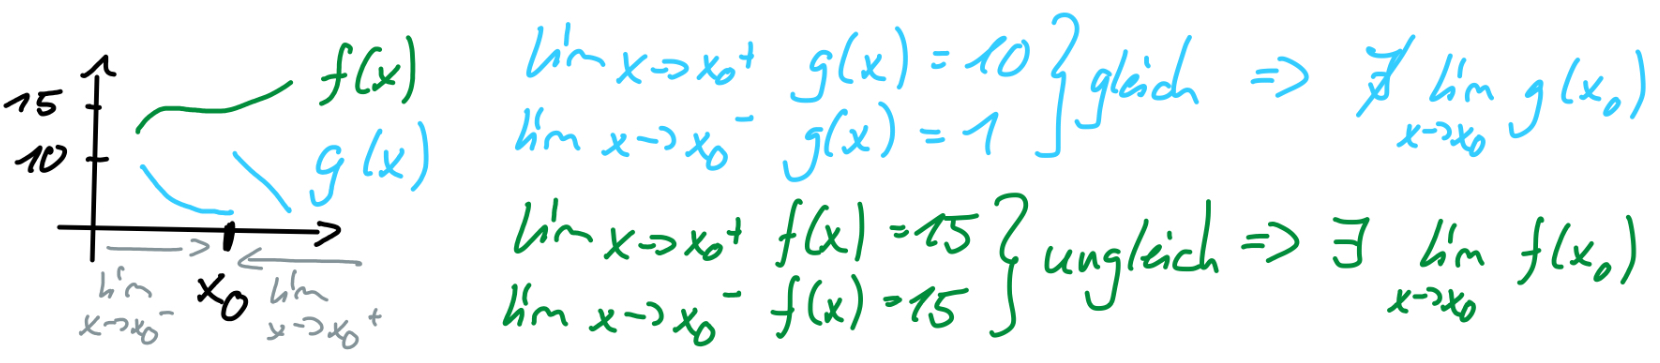
\includegraphics[scale=0.1]{linksrechtsseitigergrenzwert.jpeg}
\begin{itemize}[leftmargin=4.5mm, topsep=1pt, parsep=1pt]
    \item \textbf{Rechtsseitiger Grenzwert:} $\lim_{x \to x_0^+}$ \\
          falls Grenzwert der eingeschränkten Funktion $f|_{\mathbb{D} \cap [x_0, +\infty[}$ für $x \to x_0$ existiert. \\
          Wobei $x_0 \in \R$ ein Häufigkeitspunkt von $\mathbb{D} \cap ]x_0, + \infty[$.
    \item \textbf{Linksseitiger Grenzwert:} $\lim_{x \to x_0^-}$ \\
          falls Grenzwert der eingeschränkten Funktion $f|_{\mathbb{D} \cap [-\infty, x_0[}$ für $x \to x_0$ existiert. \\
          Wobei $x_0 \in \R$ ein Häufigkeitspunkt von $\mathbb{D} \cap ]x_0, + \infty[$.
\end{itemize}

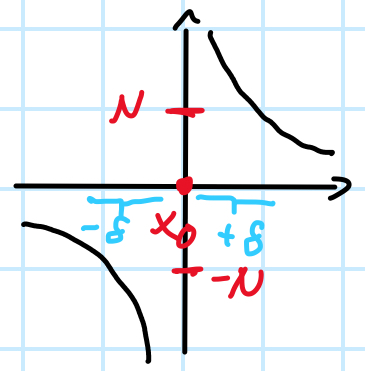
\includegraphics[scale=0.1]{linksrechtsseitigergrenzwerterweitert.jpeg}
\begin{itemize}[leftmargin=4.5mm, topsep=1pt, parsep=1pt]
    \item \textbf{Rechtsseitiger GW Erweitert:} $\lim_{x \to x_0^+} f(x) = +\infty$ \\
          falls $\forall N > 0, \ \exists \delta > 0 \ \forall x \in D \cap ]x_0, x_0 + \delta[ : f(x) > N$.
          $\iff \forall \epsilon > 0, \ \exists \delta > 0, \ \forall x \in ]x_0, x_0 + \delta[ \cap \mathbb{D} : f(x) > \frac{1}{\epsilon}$. \\
    \item \textbf{Linksseitiger GW Erweitert:} $\lim_{x \to x_0^-} f(x) = -\infty$ \\ 
          falls $\forall N > 0, \ \exists \delta > 0 \ \forall x \in D \cap ]x_0, x_0 + \delta[ : f(x) < -N$.
          $\iff \forall \epsilon > 0, \ \exists \delta > 0, \ \forall x \in ]x_0, x_0 + \delta[ \cap \mathbb{D} : f(x) < -\frac{1}{\epsilon}$. \\
\end{itemize}

\subsubsection{Unendlicher Grenzwert}
\begin{itemize}[leftmargin=4.5mm, topsep=1pt, parsep=1pt]
    \item \textbf{Oben:} Für $f: \mathbb{D} \to \R^n, \mathbb{D}$ nach oben beschränkt, so ist $\lim_{x \to +\infty} f(x) = L \in \R$ falls $\forall \epsilon > 0, \ \exists c > 0: \ \forall x \in D, \ x > c \implies |f(x) - L| < \epsilon$
    \item \textbf{Unten:} Für $f: \mathbb{D} \to \R^n, \mathbb{D}$ nach unten beschränkt, so ist $\lim_{x \to -\infty} f(x) = L \in \R$ falls $\forall \epsilon > 0, \ \exists c > 0: \ \forall x \in D, \ x < -c \implies |f(x) - L| < \epsilon$
\end{itemize}
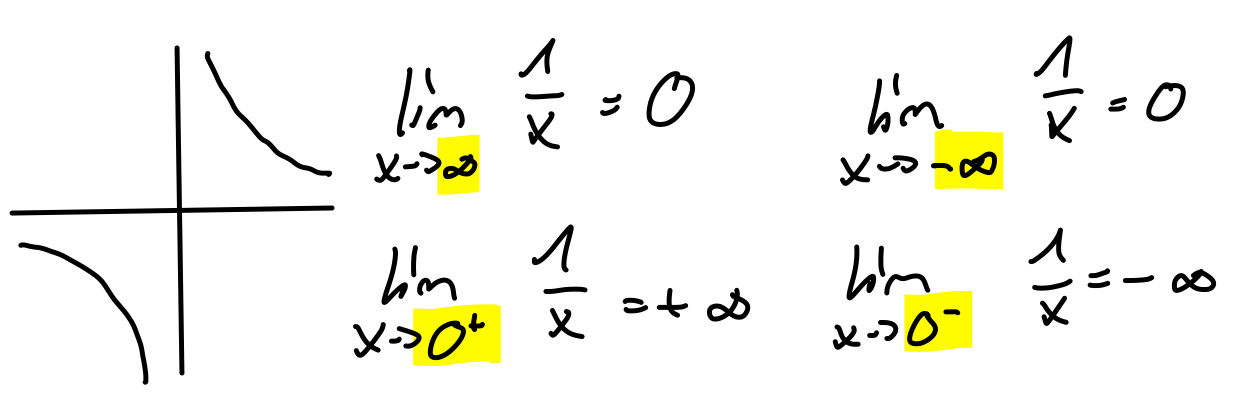
\includegraphics[scale=0.1]{unendlichergrenzwert.jpeg}


\subsubsection{weitere Eigenschaften von Grenzwerten}
\begin{mainbox}{Variablenwechsel}
  Seien $f$ und $g$ Funktionen, wobei $f$ stetig in $y_0$ und $g$ stetig in $x_0$ ist und gilt, dass $y_0 = \lim_{x \rightarrow x_0} g(x)$. Dann gilt: $\lim_{x \rightarrow x_0} f(g(x)) = \lim_{y \rightarrow y_0} f(y)$.
\end{mainbox}

\begin{mainbox}{Exponentenregel}
  Seien $f,g: D \subseteq \mathbb{R} \rightarrow \mathbb{R}$ stetig in $x_0 \in D$ mit $\lim_{x \rightarrow x_0} f(x) = f(x_0) > 0$ und $\Leftrightarrow \lim_{x \rightarrow x_0} g(x) = g(x_0)$ (beide Grenzwerte existieren). Dann gilt: $\lim_{x \rightarrow x_0} f(x)^{g(x)} = f(x_0)^{g(x_0)}$.
\end{mainbox}

\begin{howtobox}{Grenzwert nicht existiert}
  Es gilt: $\lim_{x \rightarrow a} f(x) = A \Leftrightarrow$ für jede Folge $(a_n)$ in $D \setminus \{a\}$ mit $\lim_{n \rightarrow +\infty} a_n = a$, folgt $\lim_{n \rightarrow a} f(a_n) = A$. Dadurch können wir die Existenz eines Grenzwertes widerlegen, wenn fir zwei verschiedene Folgen finden für die gilt: $\lim_{n \rightarrow \infty} a_n = a$ und $\lim_{n \rightarrow \infty} b_n = a$, aber $\lim_{n \rightarrow \infty} f(a_n) \neq \lim_{n \rightarrow \infty} f(b_n)$.
\end{howtobox}

\subsection{Trigonometrische Funktionen}
\begin{wrapfigure}{l}{0pt} 
  \definecolor{dg}{RGB}{12, 100, 0}
  \definecolor{db}{RGB}{12, 40, 150}
  \definecolor{dbt}{RGB}{20, 50, 160}
  \definecolor{dr}{RGB}{250, 0, 100}
  \definecolor{dark}{RGB}{100, 100, 100}
  \begin{tikzpicture}[scale=0.42]
    \begin{axis}%
      [grid=both,
      minor tick num=4,
      grid style={line width=.1pt, draw=gray!10},
      major grid style={line width=.2pt,draw=gray!50},
      axis lines=middle,
      enlargelimits={abs=0.4}
      ]
      \addplot[domain=-1.3:1.3,samples=50,smooth,dg] {tan(deg(x))} node[right] {$\tan(x)$};
      \addplot[domain=-6.5:6.5,samples=50,smooth,db] {sin(deg(x))};
      \addplot[domain=-2*pi:2*pi,samples=50,smooth,dr] {cos(deg(x))};
      \node[dbt, above] at (axis cs:-4.6,1) {$\sin(x)$};
      \node[dr, above] at (axis cs:-3,-1.75) {$\cos(x)$};
      \draw[-, line width=0.2mm, dark] (pi,0) -- (pi,0.25) node[above] {$\pi$};
      \draw[-, line width=0.2mm, dark] (-pi,0) -- (-pi,0.25) node[above] {$-\pi$};
      \draw[-, line width=0.2mm, dark] (2*pi,0) -- (2*pi,0.25) node[above] {$2\pi$};    
      \draw[-, line width=0.2mm, dark] (-2*pi,0) -- (-2*pi,0.25) node[above] {$-2\pi$};
      \draw[-, line width=0.1mm, dark] (pi/2,0) -- (pi/2,0.25) node[above] {$\frac{\pi}{2}$};
      \draw[-, line width=0.1mm, dark] (-pi/2,0) -- (-pi/2,0.25) node[above] {$-\frac{\pi}{2}$};
    \end{axis}
  \end{tikzpicture}
\end{wrapfigure}
$\sin(z) = z - \frac{z^2}{3!} + \frac{z^{5}}{5!} - \dots$ \\
    $\qquad = \sum_{n=0}^{\infty} \frac{(-1)^n z^{2n + 1}}{(2n + 1)!}$ \\
  \begin{compactitem}
    \item $\sin: \R \to \R$ stetig.
  \end{compactitem}
$\cos(z) = 1 - \frac{z^2}{2!} + \frac{z^{4}}{4!} - \dots$ \\ 
    $\qquad  = \sum_{n=0}^{\infty} \frac{(-1)^nz^{2n}}{(2n)!}$ \\
    \begin{compactitem}
      \item $\cos: \R \to \R$ stetig.
    \end{compactitem}

Common Values: \\
  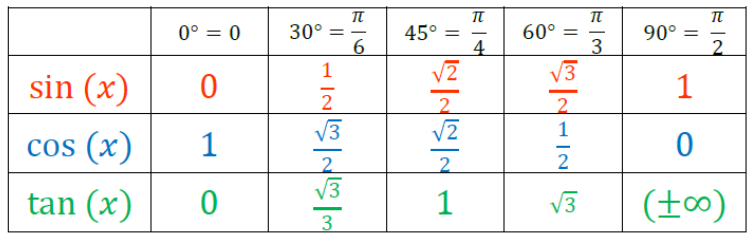
\includegraphics[scale=0.32]{SinCosTan.png}

\begin{itemize}[leftmargin=4.5mm, topsep=1pt, parsep=1pt]
  \item $\exp(iz) = \cos(x) + i \sin(z) \ \forall z \in \C$
  \item
      \begin{inparaitem}
          \item $\cos(z) = \cos(-z)$ \qquad
          \item $\sin(-z) = - \sin(z) \ \forall z \in \C$
      \end{inparaitem}
  \item
      \begin{inparaitem}
          \item $\sin(z) = \frac{e^{iz} - e^{-iz}}{2i}$ \qquad
          \item $\cos(z) = \frac{e^{iz} + e^{-iz}}{2}$
      \end{inparaitem}
  \item
      \begin{inparaitem}
          \item $\sin(z + w) = \sin(z) \cos(w) + \cos(z) \sin(w)$ \\
          \item $\cos(z + w) = \cos(z) \cos(w) - \sin(z) \sin(w)$
      \end{inparaitem}
  \item $\cos(z)^2 + \sin(z)^2 = 1 \ \forall z \in \C$
  \item
      \begin{inparaitem}
          \item $\sin(2z) = 2 \sin(z) \cos(z)$ \qquad
          \item $\cos(2z) = \cos(z)^2 - \sin(z)^2$
      \end{inparaitem}
\end{itemize}


\subsection{Kreiszahl}
\begin{itemize}[leftmargin=4.5mm, topsep=1pt, parsep=1pt]
    \item $\sin$ hat auf $]0, +\infty[$ min. eine Nullstelle.
    \item für $\pi := \inf \{t > 0 | \sin(t) = 0\} \implies$
        \begin{compactenum}
            \item $\sin(\pi) = 0 \ \pi \in ]2, 4[$
            \item $\forall x \in ]0, \pi[ : \sin(x) > 0$
            \item $e^{\frac{i\pi}{2}} = i$
        \end{compactenum}
    \item $x \ge \sin(x) \ge x - \frac{x^3}{3!} \ \forall 0 \le x \le \sqrt{6}$
\end{itemize}


Weiter gilt $\forall x \in \R$:

\begin{itemize}[leftmargin=4.5mm, topsep=1pt, parsep=1pt]
    \item
        \begin{inparaitem}
            \item $e^{i \pi} = -1$
            \item $e^{2 \pi i} = 1$
        \end{inparaitem}
    \item
        \begin{inparaitem}
            \item $\sin(x + \frac{\pi}{2}) = \cos(x)$
            \item $\cos(x + \frac{\pi}{2}) = - \sin(x)$ \\
            \item $\sin(\frac{\pi}{2} - x) = \cos(x)$
        \end{inparaitem}
    \item
        \begin{inparaitem}
            \item $\sin(x + \pi) = - \sin(x)$
            \item $\cos(x + \pi) = - \cos(x)$
        \end{inparaitem}
    \item
        \begin{inparaitem}
            \item $\sin(x + 2 \pi) = \sin(x)$
            \item $\cos(x + 2 \pi) = \cos(x)$ \\
            \item $\sin(\pi - x) = \sin(x)$
        \end{inparaitem}
    \item Nullstellen von $\sin(x) = \{k \cdot \pi | k \in \Z\}$ \\
          \tiny \color{gray} 
            $k \cdot \pi$ bedeutet, dass die Nullstellen an allen ganzzahligen Vielfachen von $\pi$ liegen. \\
          \normalsize \color{black}
          \begin{compactitem}
              \item $\sin(x) > 0, \ \forall x \in \ ] 2k \pi, (2k+1) \pi[$ 
              \item $\sin(x) < 0, \ \forall x \in \ ](2k + 1) \pi, (2k+2) \pi[$
          \end{compactitem}
      \item Nullstellen von $\cos(x) = \{\frac{\pi}{2} + k \cdot \pi | k \in \Z\}$
            \begin{compactitem}
              \item $\cos(x) > 0, \ \forall x \in \ ]\frac{-\pi}{2} + 2k\pi, \frac{-\pi}{2} + (2k+1) \pi[$
              \item $\cos(x) < 0, \ \forall x \in \ ]\frac{-\pi}{2} + (\frac{2k + 1}{2}\pi, \frac{-\pi}{2} + (2k+2) \pi[$
            \end{compactitem}
\end{itemize}

\begin{compactdesc}
    \item[Tangens:] $\tan(z) := \frac{\sin(z)}{\cos(z)}, z \not\in \{\frac{\pi}{2} + \pi k\}$
    \item[Cotangens:] $\cot(z) := \frac{\cos(z)}{\sin(z)}, z \not\in \{\pi k\}$
\end{compactdesc}

\subsection{Abbildungseigenschaften}
\begin{itemize}[leftmargin=4.5mm, topsep=1pt, parsep=1pt]
  \item \textbf{$f$ Injektiv}, $f: X \rightarrow Y$ \\
        Keine 2 verschiedenen Elemente in $X$ haben den gleichen Funktionswert in $Y$. \\
        $\forall x_1, x_2 \in X: \ x_1 \neq x_2 \Rightarrow f(x_1) \neq f(x_2)$
  \item \textbf{$f$ Surjektiv}, $f: X \rightarrow Y$ \\
        Jedes Element in $Y$ wird mind. einmal angenommen. \\
        $\forall y \in Y \ \exists x \in X : f(x) = y$ (mindestens ein $x$)
  \item \textbf{$f$ Bijektiv (= Injektiv \& Surjektiv)}, $f: X \rightarrow Y$ \\
        Perfekte Paarung. Jedes Element aus $X$ ist genau einem Element aus $Y$ zugeordnet. \\
        $\forall y \in Y \ \exists x \in X : f(x) = y$ (genau ein $x$)
\end{itemize}

\begin{bspbox}{Zeige Funktion ist Injektiv}
  $f$ ist Injektiv $\Leftrightarrow f$ streng monoton $\Leftrightarrow f'>0$ oder $f'<0$.
\end{bspbox}

\begin{bspbox}{Zeige Funktion ist Surjektiv}
  Mit Zwischenwertsatz: Sei der Bildbereich = $]a,b[$
  \begin{itemize}[leftmargin=4.5mm, topsep=1pt, parsep=1pt]
    \item[1.] $\lim_{x \rightarrow \infty} f(x) = b$ und $\lim_{x \rightarrow -\infty} = a$ zeigen
    \item[2.] Sei nun $y \in ]a,b[$ beliebig. Wegen der Grenzwerte von $f$ gilt: $\exists x_1 < x_2 : f(x_1) < y < f(x_2)$. Mit dem Zwischenwertsatz gilt dann: \\ $\exists c \in [x_1,x_2] : f(c) = y$ und somit ist $f$ surjektiv.
  \end{itemize}
\end{bspbox}

\section{Differentialrechnung}
\subsection{Vorgehen}
\begin{howtobox}{Extremaltstellen berechnen}
  \begin{itemize}[leftmargin=3mm, topsep=1pt, parsep=1pt]
    \item[1.] Erste und Zweite Ableitung berechnen (dazu Rechenregeln Ableitungen nutzen) 
    \item[2.] Implikationen der Ableitungen nutzen.
  \end{itemize}
\end{howtobox}


\subsection{Definition Differenzierbarkeit von $f$}
Funktion ist differenzierbar $\iff \forall x_i$ eine Tangente gelegt werden kann a.k.a. die Ableitung existiert.
\begin{mainbox}{$f$ in $x_0$ differenzierbar}
  $f$ ist in $x_0$ differenzierbar wenn Grenzwert $\lim_{x\to x_0} \frac{f(x) - f(x_0)}{x - x_0} = \lim_{h\to0}\frac{f(x_0+h)-f(x_0)}{h} = f'(x_0)$ existiert. 
  Dieser Grenzwert mit $f'(x_0)$ bezeichnet. Er heisst die Ableitung von f an der Stelle $x_0$\\ 
\end{mainbox}
\begin{itemize}[leftmargin=4.5mm, topsep=1pt, parsep=1pt]
  \item $f$ in $x_0$ differenzierbar, dann lässt sich linear durch die Tangente annähern.
  \item $f$ differenzierbar in $x_0 \implies f$ stetig in $x_0$. Achtung!$\notimpliedby$
\end{itemize}

\begin{mainbox}{$f$ ist differenzierbar}
  $f$ differenzierbar $\iff f$ für jedes $x_0 \in D$ differenzierbar. 
\end{mainbox}

\subsubsection{Differenzierbarkeit nach Weierstrass}
\begin{subbox}{Differenzierbarkeit nach Weierstrass}
  Sei $f:D \rightarrow \mathbb{R}, \ x_0 \in D$ ein Häufungspunkt von $D$. Dann gilt: $f$ ist in $x_0$ differenzierbar $\Leftrightarrow$ Es gibt $c \in \mathbb{R}$ und $r:D \rightarrow \mathbb{R}$ mit:
  \begin{itemize}[leftmargin=4.5mm, topsep=1pt, parsep=1pt]
    \item[1.] $f(x) = f(x_0) + c(x-x_0) + r(x)(x-x_0)$
    \item[2.] $r(x_0) = 0$ und $r$ stetig in $x_0$
  \end{itemize}
  Falls dies zutrifft ist $c = f'(x_0)$ eindeutig bestimmt.
\end{subbox}

\subsubsection{Alternative Differenzierbarkeit ohne Limes}
Sei $\Phi(x) = f'(x_o) + r(x)$:
\begin{itemize}[leftmargin=4.5mm, topsep=1pt, parsep=1pt]
    \item $f: \mathbb{D} \to \R$ ist in $x_0$ differenzierbar $\iff \exists \Phi: \mathbb{D} \to \R$ welche
        \begin{inparaenum}
            \item In $x_0$ stetig ist
            \item $f(x) = f(x_0) + \Phi(x)(x - x_0) \ \forall c \in D$.
        \end{inparaenum}
        \begin{inparaitem}
        \item In diesem Fall $\Phi(x_0) = f'(x_0)$
        \end{inparaitem}
\end{itemize}
\begin{itemize}[leftmargin=4.5mm, topsep=1pt, parsep=1pt]
    \item Für $f: \mathbb{D} \to \R$ und $x_0 \in \mathbb{D}$ Häufigkeitspunkt von $\mathbb{D}$. $f$ in $x_0$ differenzierbar $\implies f$ ist in $x_0$ stetig.
\end{itemize}

\subsection{Rechenregeln Ableitung}
Für $\mathbb{D} \subset \R$, Häufigkeitspunkt $x_0 \in \mathbb{D}$ von $\mathbb{D}$ und $f,g: \mathbb{D} \to \R$ in $x_0$ differenzierbar:
\begin{itemize}[leftmargin=4.5mm, topsep=1pt, parsep=1pt]
    \item $\mathbf{(f + g)'(x_0)} = f'(x_0) + g'(x_0)$.
    \item $\mathbf{(fg)'(x_0)} = f'(x_0)g(x_0) + f(x_0)g'(x_0)$.
    \item $\mathbf{\left( \frac{f}{g} \right)' (x_0)} = \frac{f'(x_0)g(x_0) - f(x_0)g'(x_0)}{g(x_0)^2}, \ g(x_0) \neq 0$.
    \item $\mathbf{(g \circ f)'(x_0)} = (g(f(x)))' = g'(f(x_0)) \cdot f'(x_0)$ \\  
            Für $f: \mathbb{D} \to E, g: E \to \R, \mathbb{D}, E \subset \R$, Häufigkeitspunkt $x_0 \in D$ und $f$ differenzierbar in $x_0$ und $g$ differenzierbar in $f(x_0)$.
    \item $\mathbf{(f^{-1})'(y_0)} = \frac{1}{f'(x_0)} \implies (f^{-1})'(y_0) = \frac{1}{f'(f^{-1}(y_0))}$. \\
          Für $f:\mathbb{D} \to E$ bijektiv, $x_0$ Häufigkeitspunkt, $f$ in $x_0$ differenzierbar, $f'(x_0) \neq 0$, $f^{-1}$ in $y_0 = f(x_0)$ stetig $\implies y_0$ ist ein Häufungspunkt von $E$ und $f^{-1}$ ist in $y_0$ differenzierbar.
    \item $\mathbf{(c \cdot f)'(x_0)} = c \cdot f'(x_0)$.
        \tiny \color{gray}
          Konstanter Multiplikator bleibt beim Ableiten erhalten. 
        \color{black} \normalsize
\end{itemize}

\subsection{L'Hopital Bernoulli}
Grenzwerte von Funktionen berechnen die auf einen unbestimmten Ausdruck führen: $\frac{0}{0}$, $\frac{\infty}{\infty}$, $0 \cdot \infty$, $\infty - \infty$, $0^0$, $\infty^0$, $1^{\infty}$.


\begin{mainbox}{L'Hopital Bernoulli}
  \[\lim_{x \rightarrow x_0} \frac{f(x)}{g(x)} = \lim_{x \rightarrow x_0} \frac{f'(x)}{g'(x)}\]

\end{mainbox}

\begin{bspbox}{Grenzwert der Funktion $\lim_{x \to 2} \frac{x^3 + 2x^2 -8x}{x-2}$}
    Wir bemerken, wenn $x = 2$, dann $\frac{2^3 + 2(2^2) -8\cdot2}{2-2} = \frac{0}{0}$. \\
    Wir verwenden l'hopital: $\lim_{x \to 2} \frac{3x^2 + 4x - 8}{2-2} = \lim_{x \to 2} 3x^2 + 4x -8 = 3(2^2)+4\cdot2-9 = 3 \cdot 4 = 12$ 
\end{bspbox}

\begin{bspbox}{Grenzwert der Funktion $\lim_{x \to 0} \frac{cos(x)-1}{x^2}$}
  Führt auf $\frac{0}{0}$0, darum Lhopital. 2x anwenden. \\
  $\lim_{x \to 0} \frac{\cos(x)-1}{x^2} = \lim_{x \to 0} \frac{(cos(x)-1)'}{(x^2)'} = \lim_{x \to 0} \frac{-\sin(x)}{2x} = \lim_{x \to 0} \frac{-\cos(x)}{2} = \frac{-cos(0)}{2} -\frac{1}{2}$ 
\end{bspbox}



\subsection{Konvexität}
  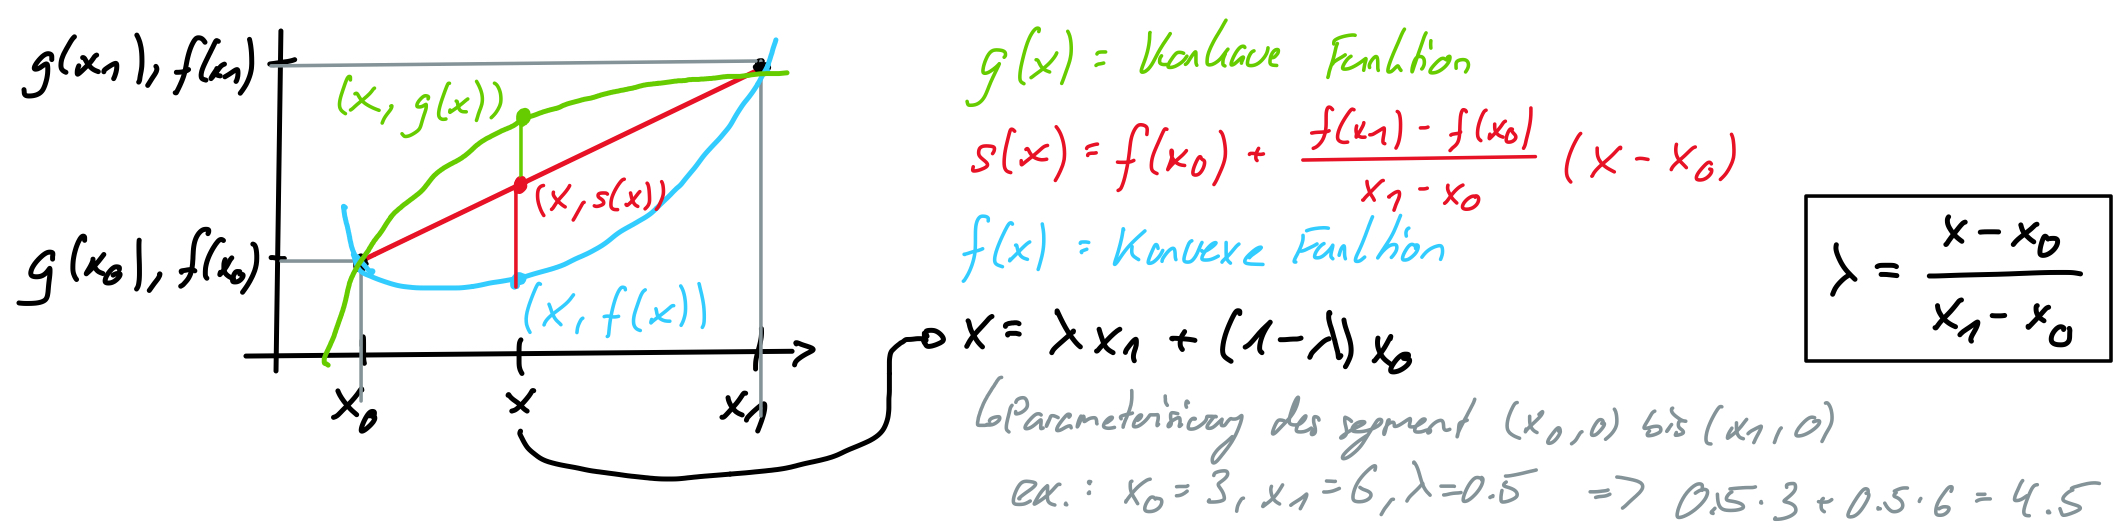
\includegraphics[scale=0.12]{konvexkonkav.jpeg} 
Für Intervall $I \subset \R$ und $f:I \to \R$. $f$ ist:
\begin{compactdesc}
    \item[Konvex:] auf $I$ falls $\forall x_0, x_1 \in I, x_0 \le x_1, \lambda \in [0, 1]$ 
          \\$ \qquad \textcolor{blue}{f(\lambda x_1 + (1- \lambda)x_0)} \le \textcolor{red}{\lambda f(x_1) + (1 - \lambda) f(x_0)}$
    \item[Streng Konvex:] falls $\forall x_0, x_1 \in I, x_0 < x_1, \lambda \in ]0, 1[,$ 
          \\ $ \qquad \textcolor{blue}{f(\lambda x_1 + (1 - \lambda)x_0)} < \textcolor{red}{\lambda f(x_1) + (1 - \lambda)f(x_0)}$
    \item[Konkav:] auf $I$ falls $\forall x_0, x_1 \in I, x_0 \le x_1, \lambda \in [0, 1],$ 
          \\ $\qquad \textcolor{green}{f(\lambda x_1 + (1- \lambda)x_0)} \ge \textcolor{red}{\lambda f(x_1) + (1 - \lambda) f(x_0)}$
    \item[Streng Konkav:] auf $I$ falls $\forall x_0, x_1 \in I, x_0 < x_1, \lambda \in [0, 1],$ 
          \\ $\qquad \textcolor{green}{f(\lambda x_1 + (1- \lambda)x_0)} \ge \textcolor{red}{\lambda f(x_1) + (1 - \lambda) f(x_0)}$
\end{compactdesc}
\begin{itemize}[leftmargin=4.5mm, topsep=1pt, parsep=1pt]
    \item $f:I \to \R$ ist konvex $\iff \forall x_0 < x < x_1 \in I, \frac{f(x) - f(x_0)}{x-x_0} \le \frac{f(x_1) - f(x)}{x_1 - x_0}$ 
          \tiny \color{gray}
            \qquad \qquad konvex $\iff$ Sekante zwischen $(f(x_0),x_0)$ \& $(x,f(x))$ hat kleinere Steigung als zwischen $(x,f(x))$ \& $(x_1,f(x_1)$
          \normalsize \color{black}
    \item Summe von zwei konvexen(/konkaven) Funktionen ist konvex(/konkav).
    \item Für $f:]a,b[ \to \R$ in $]a,b[$ differenzierbar. \\
          $f$ ist (streng) konvex $\Leftrightarrow f'$ (streng) mon. wachsend \\
          $f$ ist (streng) konkav $\Leftrightarrow f'$ (streng) mon. fallend
    \item Für $f:]a,b[ \to \R$ zwei mal differenzierbar. \\
          $f''(x) \ge 0 \iff f$ ist (streng) konvex 
\end{itemize}

\subsection{Höhere Ableitungen, Definition $f$ Glatt}
\begin{mainbox}{Höhere Ableitungen}
  \begin{itemize}[leftmargin=3mm, topsep=1pt, parsep=1pt]
    \item[1.] Für $n \geq 2$ ist $f$ $n$-mal differenzierbar in $D$ falls $f^{(n-1)}$ in $D$ differenzierbar ist. n-te Ableitung ist: $f^{(n)} = (f^{(n-1)})'$.
    \item[2.] $f$ ist $n$-mal stetig differenzierbar in $D$, falls sie $n$-mal differenzierbar ist und $f^{(n)}$ stetig in $D$ ist.
    \item[3.] $f$ ist \textbf{glatt} in $D$, falls $\forall n \geq 1$, $f$ $n$-mal in $D$ differenzierbar ist. 
        \tiny \color{gray}
          = Unendlich Differenzierbar.
        \normalsize \color{black}
  \end{itemize}
  Eine $n$-mal differenzierbare Funktion ist ($n-1$)-mal stetig differenzierbar.
\end{mainbox}

\subsubsection*{Glatte Funktionen}
$\exp(x), \ \sin(x), \ \cos(x), \ \sinh(x), \ \cosh(x), \ \tanh(x)$, $\ln(x),$ \\ $\arcsin(x). \ \arccos(x), \ arccot(x), \ \arctan(x)$ \& Polynome sind glatt. $\tan(x)$ ist auf $\mathbb{R} \setminus \{\frac{\pi}{2} + k\pi\}$, $\cot(x)$ auf $\mathbb{R} \setminus \{k\pi\}$ glatt.

\subsubsection*{Rechenregeln Höhere Ableitungen}
Für $f,g: \mathbb{D} \to \R \ n$-mal differenzierbar:
\begin{itemize}[leftmargin=4.5mm, topsep=1pt, parsep=1pt]
    \item \textbf{$\mathbf{f + g}$:} ist $n$-mal diff. und $(f + g)^{(n)} = f^{(n)} + g^{(n)}$.
    \item \textbf{$\mathbf{f \cdot g}$:} ist $n$-mal diff. und $(f \cdot g)^{(n)} = \sum_{k=0}^{n} \binom{n}{k}f^{(k)} g^{(n-k)}$.
    \item \textbf{$\mathbf{f / g}$:} ist $n$-mal diff. falls $g(x) \neq 0 \ \forall x \in \mathbb{D}$.
    \item \textbf{$\mathbf{g \circ f}$:} ist $n$-mal diff. und $(g \circ f)^{(n)}(x) =  \sum_{k=1}^{n} A_{n,k}(x)\left( g^{(k)} \circ f \right) (x), A_{n,k}$ ist ein Polynom.
\end{itemize}


\subsection{Potenzreihen Ableitungsregeln}
\begin{itemize}[leftmargin=4.5mm, topsep=1pt, parsep=1pt]
    \item Für Folge $(f_n) \in C^1, f_n \overset{\text{glm.}}{\to} f, f'_n \overset{\text{glm.}}{\to} g, f,g: ]a,b[ \to \R$. Dann $f \in C^1$ und $f'=g$. Weiter ist
        \begin{itemize}[leftmargin=4.5mm, topsep=1pt, parsep=1pt]
            \item $f$ auf $]x_0 - \rho, x_0 + \rho[$ glatt
            \item $f^{(j)} (x) = \sum_{k=1}^{\infty} c_k \frac{k!}{((k-j)!} (x - x_0)^{k-j}$
            \item $c_j = \frac{f^{(j)}(x_0)}{j!}$
        \end{itemize}
    \item Für Potenzreihe $\sum_{k=0}^{\infty} c_kx^k$ mit $\rho > 0$, dann ist
        \begin{itemize}[leftmargin=4.5mm, topsep=1pt, parsep=1pt]
            \item $f(x) = \sum_{k=0}^{\infty} c_k (x - x_0)^k$ auf $]x_0 - \rho, x_o + \rho[$ differenzierbar
              \tiny \color{gray}
                Durch Potenzreihe gegebene Funktionen ist im Konvergenzbereich differenzierbar.
              \normalsize \color{black}
            \item $f'(x) = \sum_{k=1}^{\infty} kc_k ( x - x_0)^{k-1} \ \forall x \in ]x_0 - \rho, x_0 + \rho[$
              \tiny \color{gray}
                Für durch Potenzreihe gegebene Funktion: Ableitungen im Konvergenzbereich gliedweise berechenbar.
              \normalsize \color{black}
        \end{itemize}
    \item Falls glatte Funktion $f$ in einem Intervall $]-\rho, \rho[$ die Summe iner Potenzreihe $\sum_{k=0}^{\infty} c_kx^k$ mit Konvergenzbereich $\rho$ ist $\implies c_k=\frac{f^{(k)}(0)}{k!}$.
    \item Potenzreihen $\implies$ glatte Funktion auf ihrem Konvergenzbereich.
\end{itemize}

\subsection{Sattelpunkt und Wendepunkt}
\begin{wrapfigure}{r}{0.0\textwidth} 
  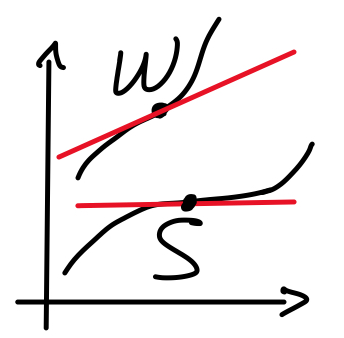
\includegraphics[scale=0.1]{satelpunktwendepunkt.jpeg} 
\end{wrapfigure}
Stelle $x_0$ wo $f'(x_0)=0$ aber kein Extremum.
\begin{compactdesc}
    \item[Wendepunkt:]
        \begin{inparaitem}
            \item $f''(x_0)=0$
            \item $f'(x_0)\neq_0$
        \end{inparaitem}
    \item[Sattelpunkt:]
        \begin{inparaitem}
            \item $f'(x_0) = 0$
            \item $f''(x_0) = 0$
        \end{inparaitem}
\end{compactdesc}

\subsection{Extremaltstellen}
Für $n \ge 0, a < x_0 < b, f:[a,b] \to \R$ in $]a,b[ \ (n+1)$-mal stetig differenzierbar und $f'(x_0) = f^{(2)}(x_0) = \dots = f^{(n)}(x_0) = 0$. Falls
\begin{itemize}[leftmargin=4.5mm, topsep=1pt, parsep=1pt]
    \item $n$ gerade und $x_0$ lokales Extremum $\implies f^{(n+1)}(x_0) = 0$
    \item $n$ ungerade und und $f^{(n+1)}(x_0) > 0 \implies x_0$ ist eine strikte lokale Minimalstelle.
    \item $n$ ungerade und und $f^{(n+1)}(x_0) < 0 \implies x_0$ ist eine strikte lokale Maximalstelle.
\end{itemize}

Für $f:[a,b] \to \R$ stetig und in $]a,b[$ zweimal stetig differenzierbar. Für $a < x_0 < b$ und $f'(x_0) = 0$. Falls
\begin{itemize}[leftmargin=4.5mm, topsep=1pt, parsep=1pt]
    \item $f^{(2)}(x_0) > 0 \implies x_0$ ist ein strike lokale Minimalstelle.
    \item $f^{(2)}(x_0) < 0 \implies x_0$ ist ein strike lokale Maximalstelle.
\end{itemize}


\subsection{Implikationen der Ableitungen}
\begin{table}[h!]
    \resizebox{0.8\linewidth}{!}{
          \begin{tabular}{c | c | c | c | l |}
            $f(x)$            & $f'(x)$  & $f''(x)$ & $ f'''(x)$ & Eigenschaft \\\hline
            $= 0$             &          &          &            & Nullstelle\\\hline
            $= 0$             & $= 0$    & $\neq 0$ &            & $2$-fache Nullstelle\\\hline
                              & $> 0$    &          &            & Strikt Monoton Steigend\\\hline
                              & $< 0$    &          &            & Strikt Monoton Fallend\\\hline
                              & $= 0$    & $< 0$    &            & Lokales Maximum\\\hline
                              & $= 0$    & $> 0$    &            & Lokales Minimum\\\hline
                              & $\neq 0$ & $= 0$    & $> 0$      & Wendepunkt r $\to$ l\\\hline
                              & $\neq 0$ & $= 0$    & $< 0$      & Wendepunkt l $\to$ r\\\hline
                              & $= 0$    & $= 0$    & $> 0$      & Sattelpunkt r $\to$ l\\\hline
                              & $= 0$    & $= 0$    & $< 0$      & Sattelpunkt l $\to$ r\\\hline
                              &          & $> 0$    &            & Streng Konvex\\\hline
                              &          & $< 0$    &            & Streng Konkav\\\hline
          \end{tabular}
    }
\end{table}


\subsubsection*{Korrolar Implikationen der Ableitung}
Seien $f,g :[a,b]\to \mathbb{R}$ stetig und in $]a,b[$ differenzierbar und \textbf{für alle} $\xi \in[a,b]$ gilt. (gilt für alle $x,x_1,x_2\in [a,b]$)
\begin{itemize}[leftmargin = 4.5mm, topsep=1pt, parsep=1pt]
	\item $f'(\xi)=0$, dann ist $f$ konstant.
	\item $f'(\xi)=g'(\xi)$, dann gibt es $c\in \mathbb{R}$ mit $f(x)=g(x)+c$
	\item $f'(\xi) > 0$, dann ist $f$ auf $[a,b]$ streng mon. wachsend.
	\item $f'(\xi)\geq 0$, dann ist $f$ auf $[a,b]$ monoton wachsend.
	\item $f'(\xi) < 0$, dann ist $f$ auf $[a,b]$ streng mon. fallend.
	\item $f'(\xi)\leq 0$, dann ist $f$ auf $[a,b]$ monoton fallend.
	\item $\exists M \geq f'(\xi)$, dann gilt $|f(x_1)-f(x_2)|\leq M|x_1-x_2|$.
	\tiny \color{gray}
    Wenn Ableitung obere Schranke $M$ hat, dann ist der Abstand der Funktionswerte immer kleiner als $M$ $\cdot$ Abstand der Argumente.
  \normalsize \color{black}
\end{itemize}


\subsection{Satz von Rolle}
\begin{subbox}{Satz von Rolle}
  \begin{wrapfigure}{r}{0.12\textwidth} 
    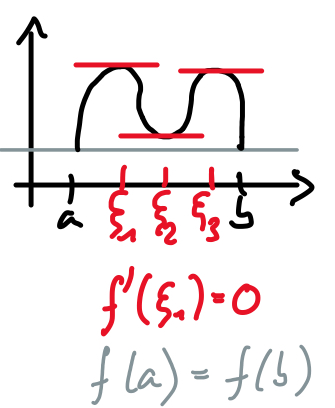
\includegraphics[scale=0.12]{satzvonrolle.jpeg} 
  \end{wrapfigure}
  Sei $f: [a,b] \to \R$ stetig und in $]a,b[$ differenzierbar. Wenn $f(a) = f(b)$ \\
  $\iff \exists \xi \in ]a,b[$ mit $f'(\xi) = 0$. \\
  \tiny \color{gray}
    Wenn differenzierbare funktion an Punkten a und b den selben Wert annimmt, dann muss es Punkte geben wo $f'(\xi) = 0$. 
  \normalsize \color{black}
\end{subbox}

\subsection{Mittelwertsatz (Lagrange)}
Es gibt im Intervall $[a,b]$ mindestens einen Punkt, wo Tangente parallel zur Sekante durch $a$ und $b$. 
\begin{mainbox}{Mittelwertsatz (Lagrange)}
  \begin{wrapfigure}{r}{0.3\textwidth} 
    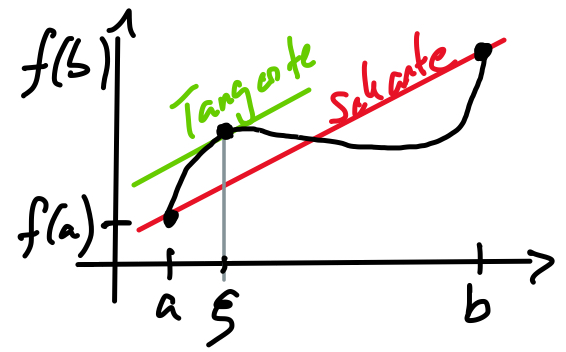
\includegraphics[scale=0.15]{mittelwertsatz.jpeg}
  \end{wrapfigure}
  Sei $f: [a,b] \to \R$ stetig und in $]a,b[$ differenzierbar. Dann gibt es $\xi \in ]a,b[$ mit $f(b) - f(a) = f'(\xi)(b-a)$. \\
  $f'(\xi) = \frac{f(b) - f(a)}{b-a}$
\end{mainbox}

\subsection{Taylor Approximation}
Taylorreihen sind ein Weg, glatte Funktionen als Potenzreihen an einem Entwicklungspunkt a anzunähern. \\
\begin{mainbox}{$T_n$ Taylor-Polynom vom Grad n}
  Sei $f: I \rightarrow \mathbb{R} \in \mathbb{C}^{\infty} (n+1)$-mal differenzierbar.
  Das n-te Taylor-Polynom $T_n f(x; a)$ an einer Entwicklungspunkt $a$ ist:
  $T_n f(x; a) := \sum_{k=0}^{n} \frac{f^{(k)}(a)}{k!} \cdot (x - a)^k$ \\
  $ = f(a) + f'(a) \cdot (x-a) + \frac{f''(a)}{2!} \cdot (x - a)^2 + \ldots$ \\
  \tiny \color{gray}
    Hinweis: $f^{(k)}(a)$ = k-te Ableitung von $f$ an der Stelle $a$.
  \normalsize \color{black}
\end{mainbox}
\begin{itemize}[leftmargin=4.5mm, topsep=1pt, parsep=1pt]
  \item Entwicklungspunkt $a$ ist Punkt wo die Annäherung startet.
  \item $x$ ist der Punkt welchen man annähern möchte.
  \item Für $c < a < d$, $\forall x \in [c, d] \ \exists \xi$ zwischen $x$ \& $a$ oder $a$ \& $x$: $f(x) = T_n(f,x,a) + R_n(f,x,a)$ 
        \\ \qquad \qquad $ = \sum_{k=0}^{n} \frac{f^{(k)}(a)}{k!}(x-a)^k + \frac{f^{(n+1)}(\xi)}{(n+1)!}(x-a)^{n+1}$.\\
  \item $R_N(f,x,a) = \frac{f^{(n+1)}(\xi)}{(n+1)!}(x-a)^{n+1}$ \\
      \tiny \color{gray}
        Restglied $R_n$ ist der Fehler der Approximation.
      \normalsize \color{black}
\end{itemize}

\begin{bspbox}{Beispiel Taylor Approximation $f(x) = sin(x)$}
  \begin{wrapfigure}{r}{0.2\textwidth} 
    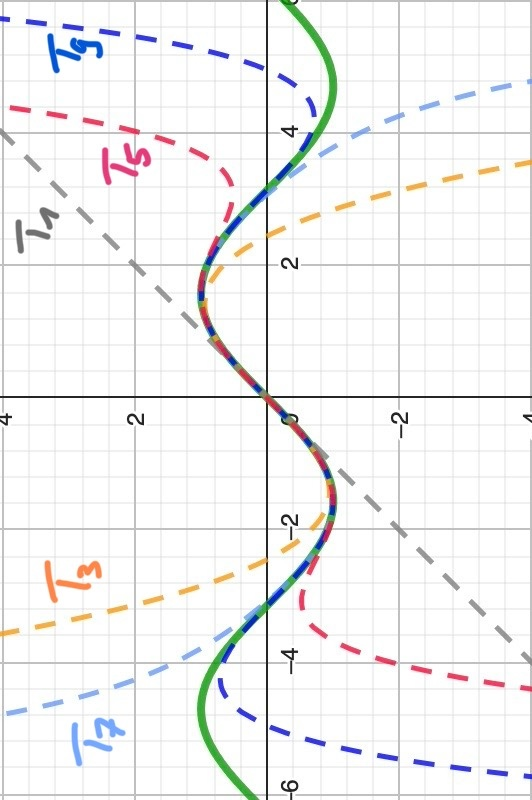
\includegraphics[scale=0.1]{tayplorpolynome.jpg}
  \end{wrapfigure}
  $T_1(x) = \sum_{k=0}^{1} \frac{f^{(k)}(a)}{k!} = \frac{f^{(0)}(0)}{0!} \cdot (x-0)^0 + \frac{f^{(1)}(0)}{1!} \cdot (x-0)^1 = 0 \cdot 1 + cos(0) \cdot x^1 = x$ \\
  $T_3(x) = \sum_{k=0}^{3} \frac{f^{(k)}(a)}{k!} = \frac{f^{(0)}(0)}{0!} \cdot (x-0)^0 + \frac{f^{(1)}(0)}{1!} \cdot (x-0)^1 + \frac{f^{(2)}(0)}{2!} \cdot (x-0)^2 + \frac{f^{(3)}(0)}{3!} \cdot (x-0)^3 =  
            \frac{-cos(0)}{3!} \cdot x^3 + \frac{-sin(0)}{2!} \cdot x^2 + \frac{cos(0)}{1} \cdot x^1 + 0 = -\frac{1}{3} \cdot x^3 + 0 + 1 \cdot x^1 = -\frac{x^3}{3!} + x$
\end{bspbox}
    
\begin{mainbox}{Taylorreihe von $f$ an Stelle $a$}
  $f \in \mathbb{C}^{\infty}$ kann auch als unendliche Reihe dargestellt werden: \\
  $Tf(x;a) := T_\infty = \sum_{k=0}^{\infty} \frac{f^{(k)}(a)}{k!} \cdot (x-a)^k$
\end{mainbox}
\begin{itemize}[leftmargin=4.5mm, topsep=1pt, parsep=1pt]
  \item Taylorreihe von $f \in C^\infty$ ist Potenzreihe mit Konvergenzradius $\rho$. 
  \item Taylorreihe konvergent $\notimplies T_\infty(x, a)$ konvergent gegen $f$.
\end{itemize}

\subsubsection*{Wichtige Taylorreihen \normalfont{(für $a=0$)}}
 \begin{inparaitem}
      \item $e^x = \sum_{n=0}^{\infty}\frac{x^n}{n!}, \forall x \in \mathbb{R}$
      \quad
      \item $e^{-x} = \sum_{n=0}^{\infty} (-1)^n \cdot \frac{x^n}{n!}, \forall x \in \mathbb{R}$
      \\
      \item $\sin(x) = \sum_{n=0}^{\infty} (-1)^n \cdot \frac{x^{2n+1}}{(2n+1)!}, \forall x$ \\
      \item $\cos(x) = \sum_{n=0}^{\infty}(-1)^n \cdot \frac{x^{2n}}{(2n)!}, \forall x$
  \end{inparaitem}

\begin{bspbox}{Taylor Approximation $f(x) = x^x$}
  Sei $f(x) = x^x, \ N = 3,$ und $x_0 = 1$. Suche die Approximation für $\left(\frac{7}{5}\right)^{\frac{7}{5}} (\Rightarrow \frac{x}{x} \Longrightarrow x = \frac{7}{5})$.
  \begin{itemize}[leftmargin=3.5mm, topsep=1pt, parsep=1pt]
    \item[1.] $f'(x), \ f''(x)$ und $f'''(x)$ berechnen.
    \item[2.] $f(x) = f(x_0) + f'(x_0)(x-1) + \frac{f''(x_0)}{2}(x-1)^2 \\ + \frac{f'''(x_0)}{6}(x-1)^3$
    \item[3.] $f(\frac{7}{5}) = 1 + \Big(\frac{7}{5}-1\Big) + \frac{2}{2}\left(\frac{7}{5}-1\right)^2 + \frac{3}{6}\left(\frac{7}{5}-1\right)^3 \\ = \frac{199}{125} = 1.592$
  \end{itemize}
\end{bspbox}


\begin{howtobox}{Rezept: Approximiere Punkt}
  Approximiere $f$ mit Entwicklungspunkt $a$ an stelle $x$ mit Taylor von Ordnung $n$
  \begin{compactenum}
      \item Leite $f \ n$ mal ab
      \item Bilder Taylorpolynom durch einsetzen von $a$ und $x$
  \end{compactenum}
\end{howtobox}

\begin{howtobox}{Rezept: Finde Fehler von Taylorpolynom}
  Gegeben Taylorpolynom $T_n(f, x, a)$ mit $n$. Ordnung.
  \begin{compactenum}
      \item Leite $f^{(n)}$ ab
  \item Bilde Restpolynom $R_N(f, x, a) = \frac{f^{(n+1)}(\xi)}{(n + 1)!}(x - a)^{n + 1}$
      \item Select $\xi \in ]a, x]$ so das $R_N(f, x, a)$ maximal ist 
  \end{compactenum}
\end{howtobox}

\section{Riemann Integral}
\subsection{Grundlagen}
\textbf{Integrieren} = Aufleiten: $f(x) \rightarrow F(x) + C$ \\
\textbf{Ableiten}: $f(x) \rightarrow f'(x)$

\subsection{Vorgehen}
\begin{howtobox}{Bestimmtes Integral berechnen}
  \begin{itemize}[leftmargin=3mm, topsep=1pt, parsep=1pt]
    \item[1.] Bruch vereinfachen (Faktorisieren, erweitern, etc.)
    \item[2.] Bekannte ableitungen einsetzen 
    \item[3.] Produkt von Funktionen? $\to$ Partielle Integration 
    \item[4.] Verkettete Funktion? $\to$ Substitution 
  \end{itemize}
\end{howtobox}

\subsection{Riemann-Summe}
\begin{wrapfigure}{r}{0.0\textwidth} 
  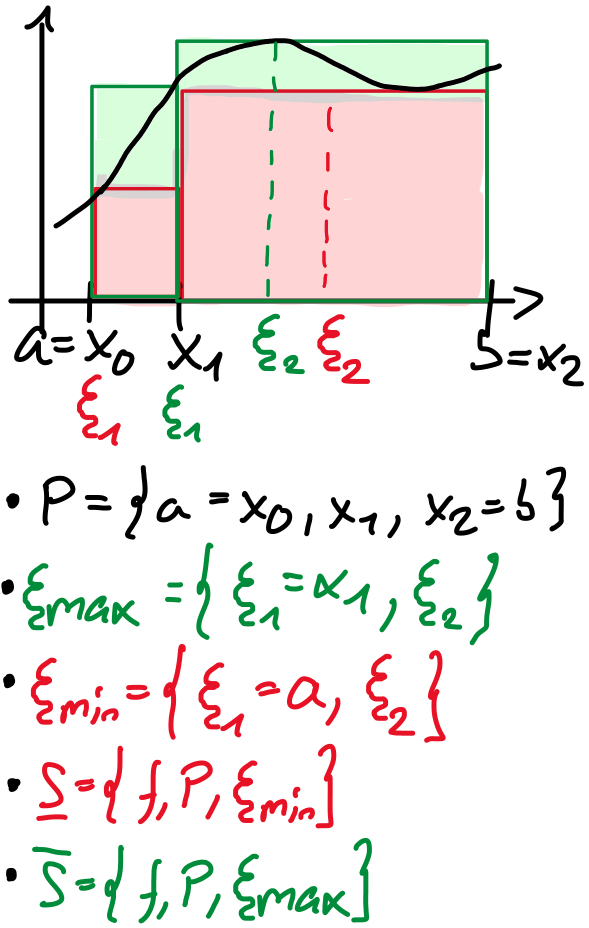
\includegraphics[scale=0.1]{riemann.jpeg}
\end{wrapfigure}
Bestimmen der Fläche unter einer Kurve.
\begin{itemize}[leftmargin=4.5mm, topsep=1pt, parsep=1pt]
  \item \textbf{Partition} $P$ ist eine endliche Teilmenge $P \subsetneq [a,b]$, $\{a,b\} \subseteq P$. \\
          $P = \{ a = x_0 < x_1 < ... < x_n = b \}$
  \item \textbf{Feinheit:} $\delta(P) := max_{1 \le i \le n} \delta_i $ \\
        \qquad \qquad \qquad $=  max_{1 \le i \le n} (x_i - x_{i-1})$ \\
        \tiny \color{gray}
          = länge des grössten Teilintervalls
        \normalsize \color{black}
  \item \textbf{$P'$ ist Verfeinerung} von $P \Leftrightarrow P \subset P'$. \\
          \tiny \color{gray}
              =$P'$ enthält mehr Punkte, unterteilt daher in mehr Abschnitte, ist deshalb genauere. 
          \normalsize \color{black}
  \item \textbf{Zwischen Punkte:} $\xi_i \in I_i$.
\end{itemize}

\begin{mainbox}{Riemann-Summe}
  Sei $f$ stetig mit $f(x): [a,b] \rightarrow \mathbb{R}$. Sei $P$ in $n$ Teile und Stützstellen $\xi$. \\
  $S(f,P,\xi) := \sum_{i=1}^n f(\xi_i) \cdot (x_i - x_{i-1})$
\end{mainbox}

\begin{subbox}{Ober- und Untersumme}
  \textbf{Untersum.:} $\underline{S}(f, P) := \sum_{i=1}^{n} (x_i - x_{i-1}) \cdot \inf_{x_{i-1} \le x \le x_i} f(x)$.\\
  \textbf{Obersum.:} $\overline{S}(f, P) := \sum_{i=1}^{n} (x_i - x_{i-1}) \cdot \sup_{x_{i-1} \le x \le x_i} f(x)$.
\end{subbox}  
\begin{itemize}[leftmargin=4.5mm, topsep=1pt, parsep=1pt]
    \item $\underline{S}(f) \le \overline{S}(f)$.
    \item $\underline{S}(f, P_1) \le \overline{S}(f, P_2) \ \forall P_1, P_2 \subset I$.  \\
            \tiny \color{gray} obersumme ist grösser als untersumme für jede beliebigen Partitionen \normalsize \color{black}
    \item $\underline{S}(f, P) \le \underline{S}(f, P') \le \overline{S}(f, P') \le \overline{S}(f, P) \ \forall P' \subset P \subset I$.
            \tiny \color{gray} wenn P' Verfeinerung von P, dann ist untersumme von P kleiner als untersumme von P' und obersumme von P' kleiner als obersumme von P \normalsize \color{black}
  \end{itemize}

\begin{subbox}{Oberes- \& Unteres Integral}
    \textbf{Unteres Integral:} $\underline{S}(f) := \sup_{P \in \mathbb{P}(I)} \underline{S}(f, P)$. \\
    \textbf{Oberes Integral:} $\overline{S}(f) := \inf_{P \in \mathbb{P}(I)} \overline{S}(f, P)$.
\end{subbox}  


\subsection{Riemann Integrierbar Kriterien}
\begin{mainbox}{$f$ Riemann-integrierbar}  
Beschränkte Funktion $f:[a,b] \to R$ ist integrierbar
  \begin{itemize}[leftmargin=4.5mm, topsep=1pt, parsep=1pt]
    \item $\iff s(f) = S(f) =: \int_{a}^{b} f(x) \mathrm{d}x$. 
      \tiny \color{gray} ($\delta_i = dx$) \normalsize \color{black} \\
      \tiny \color{gray} Integrierbar, wenn unter- und obersumme gleich sind. \normalsize \color{black}
    \item $\iff \forall \epsilon > 0 \ \exists P \in \mathbb{P}(I), S(f, P) - s(f, P) < \epsilon$.
    \item $\iff \forall \epsilon > 0 \ \exists \delta > 0: \ \forall P \in \mathbb{P}_\delta(I), S(f, P) - s(f, P) < \epsilon$.
    \item mit $A:= \int_{a}^{b} f(x) \mathrm{d}x \iff \forall \epsilon > 0 \ \exists \delta > 0: \ \forall P \in \mathbb{P}_\delta(I), \ \xi_i \in [x_{i-1}, x_i], \ \left| A - \sum_{i=1}^{n} f(\xi_i) \delta_i \right| < \epsilon$.
    \item $\iff \exists \lim_{\delta{P} \to 0} S(f, P, \xi) =: \int_{a}^{b} f(x) \mathrm{d}x$.
  \end{itemize}
\end{mainbox}
\begin{itemize}[leftmargin=4.5mm, topsep=1pt, parsep=1pt]
    \item $f: [a, b] \to \R$ stetig $\implies f$ auf $[a,b]$ integrierbar.
          \tiny \color{gray} Jede stetige funktion auf kompaktem Intervall ist integrierbar. \normalsize \color{black} 
    \item $f: [a, b] \to \R$ monoton $\implies f$ auf $[a,b]$ integrierbar.
    \item $a < b < c, f: [a, c] \to \R$ beschränkt mit $f|_{[a,b]}$ und $f|_{[b,c]}$ integrierbar $\implies f$ integrierbar und $\int_{a}^{c} f(x) \mathrm{d}x = \int_{a}^{b} f(x) \mathrm{d}x + \int_{b}^{c} f(x) \mathrm{d}x$.
          \tiny \color{gray} Monotonie von Integralen \normalsize \color{black}
    \item
        \begin{inparaitem}
            \item $\int_{a}^{a} f(x)\mathrm{d}x = 0$
            \item $\int_{a}^{b} f(x)\mathrm{d}x = -\int_{b}^{a} \mathrm{d}x$
        \end{inparaitem}
    \item kompaktes Intervall $I \subset \R$ mit Endpkt. $a,b$, Funktionen $f, g : I \to \R$ beschränkt, integrierbar \& $\alpha, \beta \in \R \implies \int_{a}^{b} (\alpha f(x) + \beta g(x)) \mathrm{d}x = \alpha \int_{a}^{b} f(x) \mathrm{d}x + \beta \int_{a}^{b} g(x)\mathrm{d}x$ \& $\alpha f_1 + \beta f_2$ integrierbar.
          \tiny \color{gray} Gebietsadditivität \normalsize \color{black} 
  \end{itemize}

\subsubsection{Rechenregeln Integrierbare Funktionen}
\begin{subbox}{Weitere integrierbare Funktionen}
  Wenn $f,g$ beschränkt und integrierbar sind, dann sind
  $f+g, \ \lambda \cdot f, , \ f \cdot g, \ |f|, \ \max(f,g), \ \min(f,g), \ \frac{f}{g}$ integrierbar.
\end{subbox}

Für $f, g: [a,b] \to \R$ beschränkt integrierbar:
\begin{itemize}[leftmargin=4.5mm, topsep=1pt, parsep=1pt]
    \item falls $f(x) \le g(x) \ \forall x \in [a,b] \implies \int_{a}^{b} f(x) \mathrm{d}x \le \int_{a}^{b} g(x) \mathrm{d}x$.
    \item $\left| \int_{a}^{b} f(x) \mathrm{d}x \right| \le \int_{a}^{b} \left| f(x) \right| \mathrm{d}x$.
    \item $\left| \int_{a}^{b} f(x)g(x) \mathrm{d}x \right| \le \sqrt{\int_{a}^{b} f^2(x) \mathrm{d}x}\sqrt{\int_{a}^{b} g^2(x) \mathrm{d}x}$.
    \item Für Intervall $I \subset \R$ und $f: I \to \R$ stetig:
        \begin{itemize}[leftmargin=4.5mm, topsep=1pt, parsep=1pt]
            \item Für $a,b,c \in \R,$ Intervall $[a+c, b+c] \in I \implies \int_{a+c}^{b+c} f(x) \mathrm{d}x = \int_{a}^{b} f(t + c)\mathrm{d}t$.
            \item Für $a,b,c \in R, c \neq 0,$ Intervall $[a \cdot c, b \cdot c] \in I \implies \int_{a}^{b} f(c \cdot t) \mathrm{d}t = \frac{1}{c} \int_{ac}^{bc} f(x) \mathrm{d}x$.
        \end{itemize}
\end{itemize}

\subsection{Unbestimmtes Integral}
\begin{mainbox}{Unbestimmtes Integral}
  $\int f(x) \mathrm{d}x = F(x) + C$ \\
   \tiny \color{gray}    
       Menge aller Aufleitungen von $f(x)$ a.k.a. aller Stammfunkt. $C = $ Integrationskonstante.
   \normalsize \color{black}
\end{mainbox}


\subsection{Bestimmtes Integral}
Flächeninhalt unter der Kurve zwischen den Punkten $a$ und $b$ \\
\begin{mainbox}{Bestimmtes Integral}
   $\int_{a}^{b} f(x) \mathrm{d}x = \limn \sum_{i=1}^n f(\xi_i) \cdot (x_i - x_{i-1}) = F(b) - F(a)$ \\
   \tiny \color{gray}    
     Grenzwert der Riemann-Summe wenn Anzahl Teilintervalle $n$ gegen unendlich geht.
    \normalsize \color{black}
\end{mainbox}

\begin{bspbox}{$\int_{0}^{1} \frac{x^2 -6x +8}{x+1}$ Bestimmtes Integral berechnen}
  $\int_{0}^{1} \frac{x^2 -6x +8}{x+1} = \int_{0}^{1} (\frac{(x+1)(x-7)}{x+1} + \frac{15}{x+1}) = \int_{0}^{1} (x-7) + 15 \cdot \int_{0}^{1} \frac{1}{x+1}$
  Stammfunktion finden $\Rightarrow (\frac{1}{2} (x-7)^2) |_0^1 + 15 \cdot (\ln|x+1|) |_0^1$ \\
  $= \frac{1}{2} (1^2 -14+49) - \frac{1}{2} 49 + 15(\ln(2) - \ln(0) = 18 - 24.5 + 15 \cdot \ln(2))$


\end{bspbox}

\subsection{Mittelwertsatz für Integrale}
\begin{mainbox}{Mittelwertsatz}
  \begin{wrapfigure}{r}{0.13\textwidth} 
    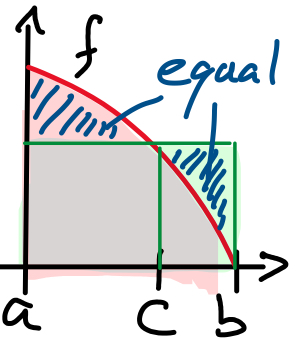
\includegraphics[scale=0.1]{riemannmittelwertsatz.jpeg}
  \end{wrapfigure}
  $f: [a,b] \to \R$ stetig \\
  $\implies \exists \xi \in [a,b]$ mit $\int_a^b f(x) \dx = f(\xi) (b-a)$.
\end{mainbox}
\begin{itemize}[leftmargin=4.5mm, topsep=1pt, parsep=1pt]
  \item für $f,g :[a,b] \to \R, f$ stetig, $g$ beschränkt integrierbar und $g(x) \ge 0 \ \forall x \in [a,b] \implies \exists \xi \in [a,b], \int_{a}^{b} f(x)g(x) \mathrm{d}x = f(\xi) \int_{a}^{b} g(x)\mathrm{d}x$.
\end{itemize}


\subsection{Stammfunktion}
\begin{subbox}{Stammfunktion $F$}
  $F: [a,b] \to \R$ ist Stammfunktion von $f$  \\
  $\iff F$ (stetig) differenzierbar in $[a,b]$ \& $F' = f$ in $[a,b]$.
\end{subbox}
''$f$ integrierbar'' impliziert \textit{nicht}, dass eine Stammfunktion existiert. Beispiel:
\begin{equation*}
  f(x) =
  \begin{cases}
    0, & \text{für } x \le 0 \\
    1, & \text{für } x > 0
  \end{cases}
\end{equation*}

\subsection{Hauptsatz Differential-/Integralrechnung}
Für stetige Funktion existiert immer eine Stammfunktion. \\
\begin{mainbox}{Hauptsatz Differential-/Integralrechnung}
  $F(x) = \int_{a}^{x} f(t) \mathrm{d}t$ ist Stammfunktion von $f$ in $[a,b]$. \\
  $\iff F'(x) = f(x) \ \forall x \in [a,b]$.\\
  \tiny \color{gray}
    Hinweis: $f$ ist stetig und Stammfunktion $F$ ist in $[a, b]$ stetig differenzierbar
  \normalsize \color{black}
\end{mainbox}

\subsection{Fundamentalsatz der Analysis}
Bestimmtes Integral von $f$ im Intervall $[a, b]$ berechnen. 
\begin{mainbox}{Fundamentalsatz der Analysis}
  \tiny \color{gray}
    $\sum_{a}^{b}F'(x) \triangle x = $
  \normalsize \color{black}
  $ \int_{a}^{b} f(x) \,dx = F(b) - F(a)$
\end{mainbox}
\subsubsection*{Polynome}
$\int c \cdot x^ndx = \frac{c \cdot x^{n+1}}{n+1}$, ($n \neq 0$)

\subsection{Integrale Berechnen}
\begin{howtobox}{Vorgehen Teil 1}
  \begin{itemize}[leftmargin=4.5mm, topsep=1pt, parsep=1pt]
    \item[1.] Verkettete Funktion? $\to$ Substitution
    \item[2.] Produkt von Funktionen? $\to$ Partielle Integration. $\sin, \ \cos$ immer $g'$ und $e$ immer $f$.
    \item[3.] Produkt von Funktionen mit $exp(x) = e^x, sin, cos$? $\to$ (Mehrmals) Partielle Integration. 
    \item[4.] Uneigentliches Integral?$\to$ nicht kompaktes Intervall Trick/unbeschränkte Funktion Trick mit anderen Werkzeugen kombinieren.
    \item[5.] Umformen: Produktregel, Kettenregel, etc.
    \item[6.] Bruchform: Vereinfachen bis Nenner von leicht integrierbaren Teilfunktionen. Partialbruchzerlegung. $\frac{u'}{2 \sqrt{u}}$ oder $\frac{u'}{u}$ erkennen ($\sqrt{u} + C, \ \log|u| + C$).
  \end{itemize}
\end{howtobox}

\begin{howtobox}{Vorgehen Teil 2}
  \begin{itemize}[leftmargin=4.5mm, topsep=1pt, parsep=1pt]
     \item[7.]Komplizierter Ausdruck mit Potenzen
              \begin{itemize}[leftmargin=3mm]
                \item[1.] $\int_a^b (f(x))^c dx$ auflösen in $\int_a^b (f(x))^{c-1} \cdot f(x) dx$ um partielle Integration anzuwenden.
                \item[2.] $\int_a^b (f(x))^c \cdot 1$ Trick anwenden um partielle Integration
                  zu benutzen.
              \end{itemize}
    \item[8.]Exponentenform
              \begin{itemize}[leftmargin=3mm]
                \item[1.] $e$ / $\log$ Trick anwenden wenn Variable $x$ in Exponent ist. erhält.
                \item[2.] z.B. $3^x = e^{\log(3) \cdot x}$
              \end{itemize}
    \item[9.] Summe im Integral: Summe aus dem Integral herausziehen. Die Reihe muss dazu gleichmässig konvergieren! \\
              Bsp. $\int_0^{\infty} \sum_{n = 0}^{\infty} \frac{(-1)^n t^{2n}}{(2n+1)!} dt = \sum_{n=0}^{\infty} \frac{(-1)^n}{(2n+1)!} \int_{0}^x t^{2n} dt$ \\ = $\sum_{n=0}^{\infty} \frac{(-1)^n x^{2n+1}}{(2n+1)!(2n+1)}$
  \end{itemize}
\end{howtobox}

\subsubsection{Partielle Integration}
Integral von produkt von Funktionen vereinfachen.
\begin{mainbox}{Partielle Integrationsregel}
  Sei $a < b$ und $f, g: [a,b] \to \R$ stetig differenzierbar. \\
  $\int_{a}^{b} f(x)g'(x)dx = f(x)g(x)|_a^b - \int_{a}^{b} f'(x)g(x)dx$ \\ 
  \tiny \color{gray}
    $= f(b)g(b)-f(a)g(a) - \int_{a}^{b} f'(x)g(x)dx$
  \normalsize \color{black}
\end{mainbox}

\begin{itemize}[leftmargin=4.5mm, topsep=1pt, parsep=1pt]
  \item Grundsätzlich leiten wir Polynome ab ($g(x)$) und sich wiederholende Funktionen ($\sin, \cos, e^x$ etc.) integrieren wir ($f'(x)$).
  \item Manchmal müssen wir künstlich mit $1$ multiplizieren, um partielle Integration anwenden zu können (Bsp. $\int \log (x) dx$)
  \item Wenn wir durch mehrfache partielle Integration wieder beim ursprünglichen Integral landen, können wir die erhaltene Gleichung nach diesem Integral auflösen.
\end{itemize}


\begin{bspbox}{$I = \int_0^1 xe^xdx$ (bestimmt, partielle Integration)}
  $I = \int_0^1 xe^xdx = fg |_0^1 - \int_0^1 f'gdx$ \\
  Wahl 1: $f(x) = x, g'(x) = e^x \implies xe^x |_0^1 - \int_0^1 1e^xdx$ (easier) \\
  $= xe^x |_0^1 - \int_0^1 e^x dx = xe^x |_0^1 - e^x |_0^1 = e-(e-1) = 1$

  \tiny \color{gray}
    Wahl 2: $f(x) = e^x, g'(x) = x \implies \frac{x^2}{2}e^x|_0^1 - \int_0^1 \frac{x^2}{2}e^xdx$ (useless) \\
  \normalsize \color{black}
\end{bspbox}

\begin{bspbox}{$I = \int \log(x) dx$ (unbestimmt, partielle Integration)}
  $I = \int ln(x)dx = \int ln(x)1dx$. Wahl: $f(x) = ln(x), g'(x) = 1$. \\
  $\implies \int ln(x)1dx = ln(x)x - \int \frac{1}{x}xdx = x \ln(x)-x + C$ \\
\end{bspbox}

\begin{bspbox}{$I = \int_{-\infty}^{0} xexp(3x) dx$ (uneigentlich, partielle Integration)}
  $I = \int_{-\infty}^{0} xexp(3x)dx =  \int_{-\infty}^{0} xe^{3x} dx$. \\
  Wahl: $f(x) = e^{3x}, g'(x) = x$ \\
  $ = (\frac{1}{2} x^2e^{3x})|_{-\infty}^0 - \int_{-\infty}^{0}(e^{3x} \frac{1}{2}x^2) = (\frac{1}{2} x^2e^{3x})|_{-\infty}^0 - (e^{3x}\frac{1}{6}x^3)|_{-\infty}^0$
  $ = \lim_{b \to \infty} \int_{-b}^{0} xe^{3x}dx$ \qquad (Uneigentlich Trick)  \\
  $= \lim_{b \to \infty} (\frac{1}{2} x^2e^{3x})|_{-b}^0 - (e^{3x}\frac{1}{6}x^3)|_{-b}^0$ 
  $ = \lim_{b \to \infty} \frac{1}{2}b^2 \cdot \frac{1}{e^{3b}} - \frac{1}{e^{3b}} \cdot \frac{1}{6}(-b)^3 = \lim_{b \to \infty} \frac{1}{e^{3b}} (\frac{b^2}{2} \cdot 1 -\frac{(-b)^2}{6} \cdot 1) = 0$
\end{bspbox}

\subsubsection{Substitution}
Integral mit verketteten Funktionen vereinfachen. \\
\begin{mainbox}{Substitutionsregel}
  Für $a < b, \ \phi: [a, b] \to \R$ stetig differenzierbar, Intervall $I \subset \R$ mit $\phi([a,b]) \subset I$ und $f: I \to \R$ stetig 
  $\implies \int_{a}^{b} f(\phi(t)) \ \phi'(t) \mathrm{d}t = \int_{\phi(a)}^{\phi(b)} f(x) \mathrm{d}x$ .
\end{mainbox}

\begin{itemize}[leftmargin=4.5mm, topsep=1pt, parsep=1pt]
    \item 2 Richtungen: 
      \begin{itemize}[leftmargin=4.5mm, topsep=1pt, parsep=1pt]
        \item $\int_{a}^{b} f(\phi(t)) \ \phi'(t)\mathrm{d}t$ (Produkt von Funktion \& Ihrer Ableitung)  $\implies$ Anwendung von links nach rechts.
        \item Integral in der Form $\int_{\alpha}^{\beta} f(x) \mathrm{d}x \implies$ Anwendung von rechts nach links $\implies$ versuch einer Substitution mittels $x = \phi(t)$, wobei $\phi(t_0) = \alpha$ und $\phi(t_1) = \beta$. \\
             \tiny \color{gray}
                Das muster wie bei Links nach Rechts ist nicht zu erkennen. 
            \normalsize \color{black}
      \end{itemize}
    \item \textit{Achtung!} Bei beiden Richtungen beachten, dass die ursprünglichen Grenzen im Integral von $t$, nun für $x$ angepasst werden müssen.
    \item Unbestimmtes integral $\int f(x) \mathrm{d}x |_{x=\phi(t)} = \int f(\phi(t))\phi'(t) \mathrm{d}t + c$.
\end{itemize}

\begin{bspbox}{$\int_0^1(1+t^2)^{2022} \cdot t \cdot dt$ mit Substitution (Links nach Rechts)}
  1. Innere Funktion substitutieren und dx berechnen: \\
  $\phi(t) = 1+t^2 = x, \phi'(t) = 2t = \frac{dx}{dt} \Rightarrow dx = 2tdt, f(x) = x^{2022}$ \\
  2. Erkenne Muster der linken Seite. $\phi'(t)$ ist in $t$ versteckt: \\
  $\int_0^1(1+t^2)^{2022} \cdot t \cdot dt = \int_0^1(1+t^2)^{2022} \cdot \frac{1}{2} \cdot 2t \cdot dt$ \\
  3. Substitutionsregel mit Grenzen für $x = \phi(x)$ angepasst: $\phi(0) = 1$ \& $\phi(1) = 2$
  $\implies \frac{1}{2} \cdot \int_{\phi(0)}^{\phi(1)} x^{2022}dx =  \int_{1}^{2} x^{2022}dx$
  4. Wert des Integrals berechnen: $= \frac{x^{2023}}{2 \cdot 2023} |_{1}^{2} = \frac{2^{2022}}{2023} - \frac{1}{2 \cdot 2023}$ \\
\end{bspbox}




\begin{bspbox}{$\int \frac{e^{\frac{1}{x}}}{x^2}dt$ mit Substitution (Links nach Rechts)}
  1. Innere Funktion substitutieren und dx berechnen: \\
  $\phi(t) = \frac{1}{t} = x, \phi'(t) = -\frac{1}{t^2} = \frac{dx}{dt} \Rightarrow dx = -t^2dt$ \\
  2. Erkenne Muster der linken Seite. $\phi'(t)$ ist in $\frac{1}{t^2}$ versteckt. \\
  $\int e^{\frac{1}{t}} \cdot \frac{1}{t^2} \cdot dt = \int e^{\frac{1}{t}} \cdot -1 \cdot -\frac{1}{t^2} \cdot dt$ \\
  3. Substitutionsregel. $= -1 \cdot \int e^{x}dx = -e^x + C = -e^{\frac{1}{t}} + C$ \\
\end{bspbox}





\begin{bspbox}{$\int_0^1 \sqrt{1-x^2}dx$ mit Substitution (Rechts nach Links)}
  Wir nutzen die trigonometrische eigenschaft $sin^2 + cos^2 = 1$ \\ 
  $\implies 1-sin^2 = cos^2$ um die Wurzel zu eliminieren: \\
  $\sin(t) = x, \qquad \cos(t)dt = dx$ \\
  $\int_0^1 \sqrt{1-x^2}dx = \int_0^{\frac{\pi}{2}} \sqrt{1-\sin^2(t)} \cos(t)dt$ \\
  $ = \int_{0}^{\frac{\pi}{2}} cos(t) \cdot cos(t) dt = \int_0^{\frac{\pi}{2}} \cos^2(t)dt$ \\
  \textit{Hinweis:} Grenzen wurden während Umformung angepasst.
\end{bspbox}

\subsection{Integration konvergenter Reihen}
\begin{mainbox}{Konvergente Reihen}
  Sei $f_n : [a,b] \rightarrow \mathbb{R}$ eine Folge von beschränkten, integrierbaren Funktionen die gleichmässig gegen eine Funktion $f: [a,b] \rightarrow \mathbb{R}$ konvergieren. So ist $f$ beschränkt integrierbar:
  $\lim_{n \rightarrow \infty} \int_a^b f_n(x) dx = \int_a^b f(x) dx$
\end{mainbox}

\begin{subbox}{$\int$ und $lim$ vertauschbar}
  Sei $f_n : [a,b] \rightarrow \mathbb{R}$ eine Folge beschränkter, integrierbarer Funktionen, sodass $\sum_{n=0}^{\infty} f_n$ auf $[a,b]$ gleichmässig konvergiert. Dann gilt: $\sum_{n=0}^{\infty} \int_a^b f_n(x) dx = \int_a^b \Big( \sum_{n=0}^{\infty} f_n(x) \Big) dx$ \\
\end{subbox}

\begin{subbox}{Integral durch Potenzreihen berechnen} 
  Sei $f(x) = \sum_{n=0}^{\infty} c_kx^k$ eine Potenzreihe mit positivem Konvergenzradius $p > 0$. Dann ist für jedes $0 \leq r < p$, $f$ auf $[-r,r]$ integrierbar und es gilt \\
  $\forall x \in \ ]-p,p[$: $\int_0^x f(t) dt = \sum_{k=0}^{\infty} c_k \cdot \frac{x^{k+1}}{k+1}$ \\
  \tiny \color{gray}
    Sei $f(x) = x^m, q = 0, b = 1$. Dann gilt: $\int_{0}^{1}f(x)dx = \int_{x}^{1}x^mdx = \frac{x^m+1}{m+1}|_0^1 = \frac{1}{m+1}$
  \normalsize \color{black}
\end{subbox}
\begin{itemize}[leftmargin=4.5mm, topsep=1pt, parsep=1pt]
  \item Potenzreihen können auf ihrem Konvergenzbereich gliedweise differenziert und integriert werden.
\end{itemize}

\subsection{Uneigentliche Integrale}
Integral berechnen für 
\begin{itemize}[leftmargin=4.5mm, topsep=1pt, parsep=1pt]
  \item unbeschränkte Funktionen 
  \item nicht kompakte Intervalle (unendliche Grenzen)
\end{itemize}

\begin{mainbox}{Uneigentliches Integral}
  Sei $f: [a, \infty] \rightarrow \R$ beschränkt\& integrierbar auf $[a,b] \forall a < b$. 
  Falls $\exists \lim_{b \rightarrow \infty} \int_a^b f(x)dx$, bezeichnen wird Grenzwert mit 
  $ \int_a^\infty f(x)dx$ und $f$ ist auf $[a, \infty[$ integrierbar.
\end{mainbox}

\begin{bspbox}{$\int_{0}^{1} \frac{1}{\sqrt{x}}dx$: unbeschränkte Funktion}
  Sinnloses Integral: $\int_{0}^{1} \frac{1}{\sqrt{x}}dx$. Weil $\frac{1}{\sqrt{x}}$ undefiniert für $x=0$. \\
  Aber $\forall \epsilon$ ist $\frac{1}{\sqrt{x}}$ auf $[\epsilon, 1]$ definiert. \\
  $\implies \int_{0}^{1} \frac{1}{\sqrt{x}}dx = \int_{\epsilon}^{1}x^{-\frac{1}{2}}dx = 2 \sqrt{x}|_\epsilon^1 = 2 \cdot 1 - 2 \cdot \sqrt{\epsilon}$. \\
  $\implies \lim_{\epsilon \to 0} \int_{\epsilon}^{1} \frac{1}{\sqrt{x}}dx = \lim_{\epsilon \to 0} 2 - 2\sqrt{\epsilon} = 2$.
\end{bspbox}

\begin{bspbox}{$\int_{0}^{\infty} x^{-2}dx =\int_{0}^{\infty} \frac{1}{x^2}dx$: nicht kompaktes Intervall}
  Sinnloses Integral: $\int_{0}^{\infty} \frac{1}{x^2}dx$. Weil Grenzwert $\infty$ \\
  Aber $\forall b$ ist $\int_{1}^{b} x^{-2}dx = -\frac{1}{x}|_1^b = -\frac{1}{b} + 1 = 1 - \frac{1}{b}$ \\
  $\implies \lim_{b \to \infty} \int_{1}^{b} x^{-2}dx = \lim_{b \to \infty} 1 - \frac{1}{b} = 1$.
\end{bspbox}

\subsubsection{Konverg./Diverg. von uneigentlichen Integralen}
\textbf{Konvergent:} falls Integral existiert (d.h. Grenzwert $\in \R$ ) \\
\textbf{Divergent:} andernfalls

\begin{mainbox}{Vergleichssatz \tiny (Majoranten-/Minorantenkriterium)} \
  $f,g: \ ]a,b[ \ \rightarrow \mathbb{R}$ stetig mit $f(x) \leq g(x) \ \forall x \in \ ]a,b[$
  \begin{itemize}[leftmargin=4.5mm, topsep=1pt, parsep=1pt]
    \item $\int_a^b g(x)dx$ konvergent $\Rightarrow \int_a^b f(x)dx$ konvergent
    \item $\int_a^b f(x)dx$ divergent $\Rightarrow \int_a^b g(x)dx$ divergent
  \end{itemize}
\end{mainbox}

\begin{mainbox}{Leibnitz-Kriterium}
  \begin{itemize}[leftmargin=4.5mm, topsep=1pt, parsep=1pt]
    \item[1.] Sei $f(x)$ auf $[a, \infty [$ stetig, monoton fallend und sei $\lim_{x \rightarrow \infty} f(x) = 0$, dann konvergieren die Integrale $\int_a^{\infty} f(x)\sin(x)dx$ und $\int_a^{\infty} f(x)\cos(x)dx$.
    \item[2.] Sei $f(x)$ auf $]a,b]$ stetig. Ist $f(x)(x-a)^2$ monoton wachsend und gilt $\lim_{x \rightarrow a^+} f(x)(x-a)^2 = 0$
      \begin{itemize}[leftmargin=4.5mm, topsep=1pt, parsep=1pt]
        \item $\implies \int_a^b f(x)\sin (\frac{1}{x-a}) dx$ konvergiert 
        \item $\implies \int_a^b f(x)\cos(\frac{1}{x-a}) dx$ konvergiert
      \end{itemize}
  \end{itemize}
\end{mainbox}

\begin{mainbox}{} 
  $f: ]a,b] \rightarrow \R \ \forall$ Intervall $[\alpha + \epsilon, b] \ \epsilon > 0$ beschränkt \& integrierbar $\Rightarrow f$ integrierbar, falls $\exists \lim_{\epsilon \rightarrow 0^+} \int_{a + \epsilon}^b f(x)dx$. Grenzwert ist $\int_a^b f(x)dx$. 
  \tiny \color{gray}
    ex: $f(x) = \frac{1}{x}: ]0, 1]$. Nicht definiert in $x = 0$. \\
  \normalsize \color{black}
\end{mainbox} 

\begin{itemize}[leftmargin=4.5mm, topsep=1pt, parsep=1pt]
  \item $\int_{1}^{\infty} \frac{1}{x^s}dx = \lim_{b \to \infty} \int_{1}^{b} \frac{1}{x^s}dx$
      \begin{itemize}
        \item konvergiert $\iff s > 1$.
        \item konvergent gegen $\frac{1}{s-1} \iff s < 1$.
        \item divergent $\iff s \leq 1$.
      \end{itemize}
  \item $\int_{a}^{b} |f(x)|$ konvergent $\implies \mathrm{d}x\int_{a}^{b} f(x) \mathrm{d}x$ abs. konv.
  \item Für $f: [a, \infty[ \to [0, \infty[$ monoton fallend. \\
        Reihe $\sum_{n=a}^{\infty} f(n)$ konvergiert $\iff \int_{a}^{\infty} f(x) \mathrm{d}x$ konvergiert \& in diesem Fall ist $0 \le \sum_{k=a}^{\infty} f(k) - \int_{a}^{\infty} f(x) \mathrm{d}x \le f(a)$. \\
        \tiny \color{gray} 
          ex: Sei $0 < s \in \R$. Wann konvergiert Reihe $\sum_{k=2}^{\infty} \frac{1}{k(\log k)^s}$?
          Sei $f(x) = \frac{1}{x(\log x)^s}$. $f$ mon. fallend. \\
          $I = \int \frac{1}{x(\log x)^s}dx$, $u = \log x$, $\frac{du}{dx} = \frac{1}{x}$
          $ \Rightarrow \lim_{b \to \infty} \int_{2}^{b} \frac{1}{x(log x)^s}dx = \lim_{b \to \infty} \int_{\log 2}^{\log b} \frac{du}{u^s} = \int_{\log 2}^{\infty} \frac{du}{u^s}$
        \normalsize \color{black}
  \item Für beidseitig offene Intervalle müssen mir den Grenzwert unabhängig nehmen: $\int_{-\infty}^{\infty} f(x) \mathrm{d}x = \lim_{a \to -\infty} \lim_{b \to +\infty} \int_{a}^{b} f(x) \mathrm{d}x$.
  \item Gaus'sches Integral: $\int_{-\infty}^{\infty} e^{-x^2} dx = \sqrt{\pi}$.
\end{itemize}

\begin{bspbox}{$\int_{- \infty}^{\infty} \sin(x) \cdot e^{-x^2} dx$: Beidseitig offenes Intervall}
  \begin{itemize}[leftmargin=4.5mm, topsep=1pt, parsep=1pt]
    \item[1.] $\int_{- \infty}^{\infty} \sin(x) \cdot e^{-x^2} dx \\ = \int_{- \infty}^{0} \sin(x) \cdot e^{-x^2} dx + \int_{0}^{\infty} \sin(x) \cdot e^{-x^2} dx$
    \item[2.] $\lim_{b \rightarrow + \infty} \int_{0}^{b} \sin(x) \cdot e^{-x^2} dx \\ = \lim_{b \rightarrow + \infty} \frac{-\sin(b) \cdot e^{-b^2}}{b} - \frac{1}{2}\cos(b)e^{b^2}$
  \end{itemize}
\end{bspbox}


\subsection{Partialbruchzerlegung}
\begin{mainbox}{Generic Partialbruchzerlegung $f(x) = \frac{1}{4k^2 - 1}$.}
  \begin{itemize}[leftmargin=4.5mm, topsep=1pt, parsep=1pt]
    \item[1.] Nenner faktorisieren $f(x) = \frac{1}{(2k-1)(2k+1)}$.
    \item[2.] Konstrukt der Dekomposition erstellen: \\ $f(x) = \frac{A}{(2k-1)} + \frac{B}{(2k+1)}$
    \item[3.] A und B berechnen: $1 = A(2k+1)+B(2k-1)$ \\
      Implies 2 new equations: \\
        $A+B = 0$ (no k on LHS) \\
        $A-B = 1$ (if A+B = 0, then this must be 1) \\
        Adding both equations we get: \\
        $2A = 1 \implies A = \frac{1}{2},$ \qquad 
        $\frac{1}{2} + B = 0 \implies B = -\frac{1}{2}$ \\
    \item[4.] A und B einfügen um Partialbruchzerlegung zu erhalten: \\
      $f(x) = \frac{1/2}{(2k-1)} - \frac{1/2}{(2k+1)} = \frac{1}{2(2k-1)} - \frac{1}{2(2k+1)} $
  \end{itemize}
\end{mainbox}

Nutzen um Rationale Funktionen $R(x) = \frac{P(x)}{Q(x)}$ zu integrieren.
\begin{mainbox}{Partialbruchzerlegung}
  Seien $p(x), q(x)$ zwei Polynome. $\int \frac{p(x)}{q(x)}$ wird wie folgend berechnet:
  \begin{itemize}[leftmargin=4.5mm, topsep=1pt, parsep=1pt]
    \item[1.] Falls $\deg(p) \ge \deg(q)$, führe eine Polynomdivision durch. Dies führt zum Integral $\int a(x) + \frac{r(x)}{q(x)}$.
    \item[2.] Berechne die Nullstellen von $q(x)$.
    \item[3.] Pro Nullstelle: Einen Partialbruch erstellen.
      \begin{itemize}[leftmargin=4.5mm, topsep=1pt, parsep=1pt]
        \item Einfach, reell: $x_1 \to \frac{A}{x - x_1}$
        \item $n$-fach, reell: $x_1 \to \frac{A_1}{x - x_1} + \ldots + \frac{A_r}{(x-x_1)^r}$
        \item Einfach, komplex: $x^2 + px + q \to \frac{Ax + B} {x^2 + px + q}$
        \item $n$-fach, komplex: $x^2 + px + q \to \frac{A_1x+b_1}{x^2+px+q} + \ldots$
      \end{itemize}
    \item[4.] Parameter $A_1, \ldots, A_n$ (bzw. $B_1, \ldots, B_n$) bestimmen. ($x$ jeweils gleich Nullstelle setzen, umformen und lösen).
  \end{itemize}
\end{mainbox}

\subsection{Euler-McLaurin-Formel}
Summen wie $1^l + 2^l + 3^l + ... + n^l$ abzuschätzen.
Voraussetzung sind Bernoulli-Polynome $B_n(x)$ und Bernoulli-Zahlen $B_n(0)$.
Des weiteren polynomen dessen Eigenschaften sind:

\begin{inparaenum}
  \item $P'_k = P_{k-1}, k > 1$ \qquad 
  \item $\int_0^1 P_k(x)\dx = 0, \forall k \geq 1$
\end{inparaenum}

Für das $k$-te Bernoulli-Polynom gilt: $B_k(x) = k!P_k(x)$.
Definiere $B_0=1$ \& Bernoulli-Zahlen rekursiv: $B_{k-1} = \sum_{i=0}^{k-1}{k \choose i}B_i = 0$.

$\implies$ Definition Bernoulli-Polynom: $$B_k(x) = \sum_{i=0}^{k}{k \choose i}B_ix^{k-i}$$

Hier ein paar Bernoulli-Polynome: $B_0(x) = 1$, $B_1(x) = x - \frac{1}{2}$, $B_2(x) = x^2 - x + \frac{1}{6}$. Nun definieren wir noch: $$\tilde{B}_k(x) = \begin{cases}
    B_k(x)   & \forall x: 0 \leq x < 1     \\
    B_k(x-n) & \forall x: n \leq x < n + 1
  \end{cases}$$

\begin{mainbox}{Euler-McLaurin-Summationsformel}
  Sei $f: [0, n] \to \R$ $k$-mal stetig differenzierbar. Dann gilt: \\
  \begin{itemize}[leftmargin=4.5mm, topsep=1pt, parsep=1pt]
    \item Für $k = 1$: \\
          $\sum_{i = 1}^n f(i) = \int_0^n f(x) \dx + \frac{1}{2}(f(n) - f(0)) \\ + \int_0^n \tilde{B}_1(x)f'(x)\dx$
    \item Für $k>1$: \\
          $\sum_{i = 1}^n f(i) = \int_0^n f(x) \dx + \frac{1}{2}(f(n) - f(0))+$ \\
          $\sum_{j = 2}^k \frac{(-1)^j B_j}{j!}(f^{(j-1)}(n) + f^{(j-1)}(0)) + \tilde{R}_k$ \\
          wobei $ \tilde{R}_k = \frac{(-1)^{k-1}}{k!} \int_0^n \tilde{B}_k(x)f^{(k)}(x)\dx$
    \end{itemize}
\end{mainbox}

\begin{subbox}{Beispiel für Euler-McLaurin}
  $$1^l + 2^l + 3^l + ... + n^l \text{ wobei } l \geq 1, l \in \mathbb{N}$$
  Angewandt auf $f(x) = x^l$ und $k = l + 1$ folgt für alle $l \geq 1$:
  $$1^l + 2^l + 3^l + ... + n^l = \frac{1}{l + 1} \sum_{j = 0}^l (-1)^j B_j {l + 1 \choose j} n^{l+1-j}$$
\end{subbox}

\subsubsection*{Examples of Maclaurin Series}
\begin{inparaitem}[leftmargin=4mm]
  \item $e^x=1+x+\frac{x^2}{2}+\cdots$
  \item $\ln(1+x)=x-\frac{x^2}{2}+\frac{x^3}{3}-\cdots$
  \item $\sin(x)=x-\frac{x^3}{3!}+\frac{x^5}{5!}-\cdots$
  \item $\cos(x)=1-\frac{x^2}{2!}+\frac{x^4}{4!}-\cdots$
  \item $\arctan(x)=x-\frac{x^3}{3}+\frac{x^5}{5}-\cdots$
\end{inparaitem}

\subsection{Gamma-Funktion}
Funktion $n \mapsto (n-1)!$ zu interpolieren. Weil $\Gamma(n+1) = n!$ \\
\begin{mainbox}{Gamma Funktion}
 $\Gamma(s) := \int_0^\infty e^{-x}x^{s-1}\dx = (s-1)! \quad \forall s > 0$
\end{mainbox}
Gamma-Funktion konvergiert $\forall s > 0$ \& hat Eingeschaften:
\begin{inparaitem}[leftmargin=4.5mm, topsep=1pt, parsep=1pt]
  \item $\Gamma(1) = 1$
  \item $\Gamma(s + 1) = s \Gamma(s)$
  \item $\Gamma$ ist logarithmisch konvex, \\
        d.h.: $\Gamma(\lambda x + (2 - \lambda)y) \leq \Gamma(x)^\lambda \Gamma(y)^{1 - \lambda} \forall x, y > 0$ \& $0 \leq \lambda \leq 1$
\end{inparaitem}
Die Gamma-Funktion ist die einzige Funktion $]0, \infty[ \to ]0, \infty[$, die $(1), (2)$ und $(3)$ erfüllt. Zudem gilt: $$\Gamma(x) = \limn \frac{n!n^x}{x(x+1)...(x+n)} \ \ \ \forall x > 0$$

\subsection{Stirling'sche Formel}
Abschätzung der Fakultät. Mit der Euler-McLaurin-Formel kombiniert folgt
$$n! = \frac{\sqrt{2\pi n} \cdot n^n}{e^n} \cdot \exp(\frac{1}{12n}+R_3(n))$$
wobei $|R_3(n)| \le \frac{\sqrt{3}}{216}\cdot\frac{1}{n^2} \ \forall n \ge 1$

\section{Komplexe Zahlen}
\begin{mainbox}{Formen \& Operationen}
  $z = x + yi$
    \tiny \color{gray}
      Kartesische Form
    \color{black} \normalsize,
  $\overline{z} = x - iy$
    \tiny \color{gray}
      Konjugation
    \color{black} \normalsize, 
    $i = \sqrt{-1} $ \\
  $|z| = \sqrt{x^2 + y^2} = z \cdot \overline{z}$ 
    \tiny \color{gray}
      Betrag
    \color{black} \normalsize\\
  $z^{-1} = \frac{1}{z} = \frac{\overline{z}}{|z|^2}$, $\forall z \neq 0$
    \tiny \color{gray}
      Reziproke a.k.a. multiplikative Inverses
    \color{black} \normalsize
    
  $+/-: (x_1 + x_2) + (y_1 + y_2) \cdot i$ \\
  $z_1 \cdot z_2 = (x_1 + y_1i) \cdot (x_2 + y_2i) \qquad \frac{z_1}{z_2} = \frac{z_1 \cdot \overline{z_2}}{|z_2|^2}$ \\
\end{mainbox}

\begin{mainbox}{Konjugation}
  $z = x + iy \in \mathbb{C} \longrightarrow \overline{z} = x - iy \in \mathbb{C}$ \\
  Die Konjugation hat die folgenden Eigenschaften
  \begin{itemize}
    \item[i)]  $z \cdot \overline{z} = (x + iy) \cdot (x - iy) = x^2 - i^2 \cdot y^2 \\ = x^2 + y^2 = |z|^2 \Longrightarrow z^{-1} = \frac{\overline{z}}{|z|^2}$, $z \neq 0$
    \item[ii)] $\overline{(z_1 + z_2)} = \overline{z_1} + \overline{z_2}$
    \item[iii)] $\overline{(z_i \cdot z_2)} = \overline{z_1} \cdot \overline{z_2}$
  \end{itemize}
\end{mainbox}

\begin{itemize}[leftmargin=4.5mm, topsep=1pt, itemsep=1pt, parsep=1pt]
    \item Weitere Eigenschaften
    \begin{itemize}[leftmargin=4.5mm, topsep=1pt, itemsep=1pt, parsep=1pt]
      \item[i)] $|z \cdot w| = |z| \cdot |w|$
      \item[ii)] $\left| \frac{z}{w} \right| = \frac{|z|}{|w|}$, $w \neq 0$
      \item[iii)] $|z| = |\overline{z}|$
      \item[iv)] $|z + w| \leqslant |z|$
    \end{itemize} 
  \end{itemize}

\begin{mainbox}{Polarform}
  Die Polarform von $z = x + iy \in \mathbb{C}$ ($\phi \in (- \pi, \pi]$) sei
  $z = r \cdot e^{i \cdot \pi}$ 
    \tiny \color{gray}
      (Euler Form)
    \color{black} \normalsize \\
  $z = r \cdot (\cos(\phi) + i \cdot \sin(\phi))$ 
    \tiny \color{gray}
      (Trigonomical Form)
    \color{black} \normalsize
    \\
    \begin{wrapfigure}[0]{r}{0.25\textwidth}
      \centerline{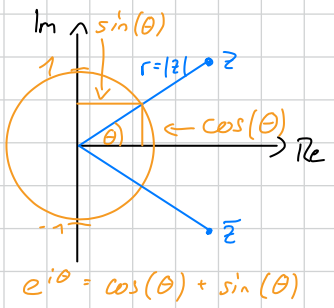
\includegraphics[scale=0.2]{polarform.png}}
      \vspace{10cm}
    \end{wrapfigure}
    mit $r = ||z|| = \sqrt{x^2 + y^2}, x = r \cdot \cos(\phi), y = r \cdot \sin(\phi)$ \\
  $\phi =
  \begin{cases}
    \arctan\left(\frac{y}{x}\right)       & x > 0                      \\
    \arctan\left(\frac{y}{x}\right) + \pi & x < 0 \wedge y \geqslant 0 \\
    \arctan\left(\frac{y}{x}\right) - \pi & x < 0 \wedge y < 0         \\
    \frac{\pi}{2}                         & x = 0  \wedge y > 0        \\
    - \frac{\pi}{2}                       & x = 0 \wedge y < 0         \\
    undefiniert                           & x = 0 \wedge y = 0         \\
  \end{cases}$
\end{mainbox}

\section{Tabellen}
\subsection{Grenzwerte von Referenzfolgen}
\tiny \color{gray}
  Bei Verwendung, schreiben "in der Vorlesung haben wir gesehen dass [FolgeX] gegen [Wert] konvergiert."
\normalsize \color{black}


\begin{table}[h!]
  \resizebox{0.8\linewidth}{!}{
      \begin{tabularx}{\linewidth}{XX}
        \toprule
        $\limxi \sqrt[n]{n} = 1$                                &                   \\
        $\limxi \frac{1}{(1+\epsilon)^n} = 0$                      & $\limxi (\frac{x}{y})^n = 0 \quad \forall x < y$                  \\
        $\limxi \frac{1}{x} = 0$                                   & $\limxi 1 + \frac{1}{x} = 1$             \\
        $\limxi e^x = \infty$                                      & $\limxn e^x = 0$                         \\
        $\limxi e^{-x} = 0$                                        & $\limxn e^{-x} = \infty$                 \\
        $\limxi \frac{e^x}{x^m} = \infty$                          & $\limxn xe^x = 0$                        \\
        $\limxi \ln(x) = \infty$                                   & $\limxo \ln(x) = -\infty$                \\
        $\limxi (1+x)^{\frac{1}{x}} = 1$                           & $\limxo (1+x)^{\frac{1}{x}} = e$         \\
        $\limxi (1+\frac{1}{x})^b = 1$                             & $\limxi n^{\frac{1}{n}} = 1$             \\
        $\lim_{x\to\pm\infty} (1 + \frac{1}{x})^x = e$             & $\limxi (1-\frac{1}{x})^x = \frac{1}{e}$ \\
        $\lim_{x\to\pm\infty} (1 + \frac{k}{x})^{mx} = e^{km}$     & $\limxi (\frac{x}{x+k})^x = e^{-k}$      \\
        $\limxo \frac{a^x -1}{x} = \ln(a), \newline \forall a > 0$ &
        $\limxi x^a q^x = 0, \newline \forall 0 \le q < 1$                                                    \\
        $\limxo \frac{\sin x}{x} = 1$                 & $\limxo \frac{\sin kx}{x} = k$     \\
        $\limxo \frac{1}{\cos x} = 1$                 & $\limxo \frac{\cos x -1}{x} = 0$   \\
        $\limxo \frac{\log 1 - x}{x} = -1$            & $\limxo x \log x = 0$              \\
        $\limxo \frac{1 - \cos x}{x^2} = \frac{1}{2}$ & $\limxo \frac{e^x-1}{x} = 1$       \\
        $\limxo \frac{x}{\arctan x} = 1$              & $\limxi \arctan x = \frac{\pi}{2}$ \\
        $\limxo \frac{e^{ax}-1}{x} = a$               & $\limxo \frac{\ln(x+1)}{x} = 1$    \\
        $\lim_{x\to 1} \frac{\ln(x)}{x-1} = 1$        & $\limxi \frac{\log(x)}{x^a} = 0$   \\
        $\limxi \sqrt[x]{x} = 1$                      & $\limxi \frac{2x}{2^x} = 0$        \\
        \bottomrule
      \end{tabularx}
  }
\end{table}


\subsection{Trivial stetige Funktionen}
\begin{inparaitem}
  \item $f(x) = c$ (c is Konstante) 
  \item $f(x) = x$ 
  \item $f(x) = x^n$
  \item $f(x) = a_nx^n + ... + a_1x + a_n$
  \item $f(x) = mx + b$ 
  \item $f(x) = ln(x)$
  \item $f(x) = exp(x)$ 
\end{inparaitem}

\subsection{Bekannte Reihen}
\resizebox{\columnwidth}{!}{\begin{tabular}{l | l | c | c | c | c}
  \multicolumn{2}{l |}{Reihe}                                      & Wert                                   & konv.               & div. &\\
  \toprule
  \multicolumn{2}{l |}{Harmonische Reihe}                          &                                        &                     & \\\hline
  $\sum_{k=1}^{\infty} \frac{1}{k}$                                &                                        & $\infty$            &                        & \checkmark \\\hline
  $\sum_{k=1}^{\infty} \frac{1}{k^2}$                              &                                        & $\frac{\pi^2}{6}$   &   \checkmark ,abs          & \\\hline
  $\sum_{k=1}^{\infty} \frac{1}{k^4}$                              &                                        & $\frac{\pi^4}{90}$  &   \checkmark ,abs           & \\\hline
  $\sum_{k=1}^{\infty} \frac{1}{k^a}$                              &                                        &                     & $a > 1$ ,abs     & $a \le 1$\\\hline
  \multicolumn{2}{l |}{Alternierende Harmon. Reihe}                &                                        &                     & \\\hline
  $\sum_{k=1}^{\infty} \frac{(-1)^{k+1}}{k}$                       &                                        & $\ln 2$             &      \checkmark        & \\\hline
  $\sum_{k=1}^{\infty} \frac{(-1)^{k+1}}{k^2}$                     &                                        & $\frac{\pi^2}{12}$  &      \checkmark ,abs       & \\\hline
  $\sum_{k=1}^{\infty} \frac{(-1)^{k+1}}{k^4}$                     &                                        & $\frac{\pi^4}{720}$ &      \checkmark ,abs       & \\\hline
  $\sum_{k=0}^{\infty} \frac{(-1)^k}{2k + 1}$                      & $1 - \frac{1}{3} + \frac{1}{5} -$      & $\frac{\pi}{4}$     &      \checkmark        & \\\hline
  \multicolumn{1}{l |}{Teleskopreihe}                              &                                        &                     & \\\hline
  $\sum_{k=1}^{\infty} \frac{1}{k(k+1)}$                           &                                        & $1$                 &      \checkmark ,abs       & \\\hline
  \multicolumn{3}{l |}{Exponentialfunktion $z \in \C,$ konv. abs.} &                                        & \\\hline
  $\sum_{k=0}^{\infty} \frac{z^k}{k!}$                             & $1 + z + \frac{z^2}{2!} +$             & $\exp{z}$           &      \checkmark ,abs     & \\\hline
  $\sum_{k=0}^{\infty} \frac{(-a)^k}{k!}$                          &                                        & $\frac{1}{e^a}$       &    \checkmark ,abs         & \\\hline
  $\sum_{k=0}^{\infty} (-1)^k\frac{x^{2k+1}}{(2k+1)!}$             & $x -\frac{x^3}{3!} + \frac{x^5}{5!} -$ & $ \sin x$           &      \checkmark ,abs      & \\\hline
  $\sum_{k=0}^{\infty} (-1)^k\frac{x^{2k}}{(2k)!}$                 & $1-\frac{x^2}{2}+\frac{x^4}{4!}-$      & $\cos x$            &      \checkmark ,abs      & \\\hline
  $\sum_{k=0}^{\infty} \frac{x^{2k+1}}{(2k+1)!}$                   & $x+\frac{x^3}{3!}+\frac{x^5}{5!}+$     & $\sinh x$           &      \checkmark ,abs      & \\\hline
  $\sum_{k=0}^{\infty} \frac{x^{2k}}{(2k)!}$                       & $1+\frac{x^2}{2}+\frac{x^4}{4!}+$      & $\cosh x$           &      \checkmark ,abs      & \\\hline
  \multicolumn{2}{l |}{Mengoli Reihe}                          &                                        &                     & \\\hline
  $\sum_{n = 1}^\infty \frac{1}{n (n + 1)} = 1$                              &                                        & 1            &                         &  \\\hline
\end{tabular}}

\subsubsection{Geometrische Reihe}
\begin{itemize}[leftmargin=4.5mm, topsep=1pt, parsep=1pt]
  \item $\sum_{k=0}^\infty q^k$: \\
  \begin{itemize}[leftmargin=4.5mm, topsep=1pt, parsep=1pt]
    \item $|q| \ge 1$: divergiert \\ 
    \item $|q| < 1$: konvergiert zu $\frac{1}{1 - q}$\\ 
            \qquad $\implies \sum_{n = 0}^{\infty} q^n = \frac{1}{1-q}$ (Summe)
            \tiny \color{gray}
              Bsp: $\sum_{k=0}^{\infty} (\frac{1}{2})^n = \frac{1}{1-\frac{1}{2}} = 2$ \\
            \normalsize \color{black}
    \item $|q| = 1$: konvergiert zu $\infty$ $\implies \sum_{k=0}^\infty 1 = \infty$
  \end{itemize}

\item $\sum_{k=0}^{\infty} (k+1)q^k$ ,Wert: $\frac{1}{(1-q)^2}$
\end{itemize}

\subsubsection{Teleskopreihe}
\begin{itemize}[leftmargin=4.5mm, topsep=1pt, parsep=1pt]
  \item $\sumn (b_n - b_{n-1}) = \sumn \frac{1}{n(n+1)} = 1$ \\
        \begin{itemize}[leftmargin=4.5mm, topsep=1pt, parsep=1pt]
          \item $(b_n)_{n \geqslant 1}$ konvergent $\implies \sumk (b_n - b_{n-1})$ konvergent. \\
            \tiny \color{gray}
              Teleskopreihe ist konvergent, wenn zugrundeliegende Folge konvergent.
            \normalsize \color{black}
          \item $\sum_{n = 1}^{\infty} (b_n - b_{n-1}) = (\limn b_n) - b_{n-1}$ \\
            \tiny \color{gray}
              Bsp: $\sum_{n = 1}^{\infty} (b_n - b_{n-1}) = \sum_{n = 1}^{\infty} \frac{n+1}{n(n+1)} - \frac{n}{n(n+1)} = \frac{1}{n} + \frac{1}{n+1}$ \\ 
                    $= (\limn b_n) - b_{n-1} = (\limn b_n) - b_0 = (\limn \frac{1}{n}) - \frac{1}{n-1} = 0 - \frac{1}{0-1} = 1$ \\
              Bsp: $\sum_{n = 3}^{\infty} (b_n - b_{n-1}) = (\limn b_n) - b_2 = \limn \frac{1}{n} - \frac{1}{2} = -\frac{1}{2}$ \\
            \normalsize \color{black}
          \end{itemize}
\end{itemize}
               
\subsubsection{Riemann Zeta-Funktion}
\begin{itemize}[leftmargin=4.5mm, topsep=1pt, parsep=1pt]
\item $\zeta(s) = \sum_{n=1}^\infty \frac{1}{n^s}$ \qquad
  \begin{inparaitem}
    \item $s \le 1$: divergiert
    \item $s > 1$:  konvergiert
  \end{inparaitem}      
\end{itemize}

\subsubsection{Alternierende Reihe}
\begin{itemize}[leftmargin=4.5mm, topsep=1pt, parsep=1pt]
  \item $\sum_{k = 1}^{\infty} (-1)^k a_k$  \\
    \begin{itemize}[leftmargin=4.5mm, topsep=1pt, parsep=1pt]
      \item Wenn $a_k$ monoton fallend \& $\limn a_k = 0 \implies$ konvergent (Leibniz).
    \end{itemize}      
\end{itemize}

\subsection{Ableitungen}
$F'(1) = 0$ Weil Konstante verschwindet beim Ableiten. \\ 


\begin{table}[h!]
  \resizebox{0.9\linewidth}{!}{
      \resizebox{\columnwidth}{!}{\begin{tabular}{c | c | c | c | c}
        $\mathbf{F(x)}$                        & $\mathbf{f(x)}$               & $\mathbf{f'(x)}$        & $\mathbf{f^{(2)}(x)}$ & $\mathbf{f^{(3)}(x)}$\\ 
        \toprule
          $\frac{1}{6}3x^3$                      & $\frac{1}{2}3x^2$           & $3x$                   &  3 & 0 \\\hline
          $\frac{1}{6}x^3$                       & $\frac{1}{2}x^2$            & $x$                    &  1 & 0 \\\hline
          $-\frac{1}{99}x^{-99}$                 & $x^{-100}$                  & $-100x^{-101}$           \\\hline

          $\frac{x^{-a+1}}{-a+1}$                & $\frac{1}{x^a}$             & $\frac{a}{x^{a+1}}$      \\\hline
          $\frac{x^{a+1}}{a+1}$                  & $x^a \ (a \ne 1)$           & $a \cdot x^{a-1}$        \\\hline
          $\frac{1}{k \ln(a)}a^{kx}$             & $a^{kx}$                    & $ka^{kx} \ln(a)$         \\\hline
          $\ln |x|$                              & $\frac{1}{x}$               & $-\frac{1}{x^2}$         \\\hline
          $\frac{2}{3}x^{3/2}$                   & $\sqrt{x}$                  & $\frac{1}{2\sqrt{x}}$    \\\hline
          $-\cos(x)$                             & $\sin(x)$                   & $\cos(x)$                \\\hline
          $\sin(x)$                              & $\cos(x)$                   & $-\sin(x)$               \\\hline
          $\frac{1}{2}(x-\frac{1}{2}\sin(2x))$   & $\sin^2(x)$                 & $2 \sin(x)\cos(x)$       \\\hline
          $\frac{1}{2}(x + \frac{1}{2}\sin(2x))$ & $\cos^2(x)$                 & $-2\sin(x)\cos(x)$       \\\hline
          $-\ln|\cos(x)|$                        & $\tan(x)$                   & $\frac{1}{\cos^2(x)}$    \\\hline
          $\log(\cosh(x))$                       & $\tanh(x)$                  & $\frac{1}{\cosh^2(x)}$   \\\hline
          $\ln | \sin(x)|$                       & $\cot(x)$                   & $-\frac{1}{\sin^2(x)}$   \\\hline
          $\frac{1}{c} \cdot e^{cx}$             & $e^{cx}$                    & $c \cdot e^{cx}$         \\\hline
          $x(\ln |x| - 1)$                       & $\ln |x|$                   & $\frac{1}{x}$            \\\hline
          $\frac{1}{2}(\ln(x))^2$                & $\frac{\ln(x)}{x}$          & $\frac{1 - \ln(x)}{x^2}$ \\\hline
          $\frac{x}{\ln(a)} (\ln|x| -1)$         & $\log_a |x|$                & $\frac{1}{\ln(a)x}$      \\\hline
          $\arcsin(x)$                           & $\frac{1}{\sqrt{1 - x^2}}$  &                         \\\hline
          $\arccos(x)$                           & $\frac{-1}{\sqrt{1 - x^2}}$ &                         \\\hline
          $\arctan(x)$                           & $\frac{1}{1 + x^2}$         &                         \\\hline
          $x^x \ (x > 0)$                        & $x^x \cdot (1 + \ln x)$     &                         \\\hline
      \end{tabular}}
}
\end{table}

\subsection{Integrale}
\begin{center}
  \begin{tabularx}{\linewidth}{>{\centering\arraybackslash}X>{\centering\arraybackslash}X}
    \toprule
    $\mathbf{f(x)}$                      & $\mathbf{F(x)}$                                                  \\
    \midrule
    $\int f'(x) f(x) \dx$                & $\frac{1}{2}(f(x))^2$                                            \\
    $\int \frac{f'(x)}{f(x)} \dx$        & $\ln|f(x)|$                                                      \\
    $\int_{-\infty}^\infty e^{-x^2} \dx$ & $\sqrt{\pi}$                                                     \\
    $\int (ax+b)^n \dx$                  & $\frac{1}{a(n+1)}(ax+b)^{n+1}$                                   \\
    $\int x(ax+b)^n \dx$                 & $\frac{(ax+b)^{n+2}}{(n+2)a^2} - \frac{b(ax+b)^{n+1}}{(n+1)a^2}$ \\
    $\int (ax^p+b)^n x^{p-1} \dx$        & $\frac{(ax^p+b)^{n+1}}{ap(n+1)}$                                 \\
    $\int (ax^p + b)^{-1} x^{p-1} \dx$   & $\frac{1}{ap} \ln |ax^p + b|$                                    \\
    $\int \frac{ax+b}{cx+d} \dx$         & $\frac{ax}{c} - \frac{ad-bc}{c^2} \ln |cx +d|$                   \\
    $\int \frac{1}{x^2+a^2} \dx$         & $\frac{1}{a} \arctan \frac{x}{a}$                                \\
    $\int \frac{1}{x^2 - a^2} \dx$       & $\frac{1}{2a} \ln\left| \frac{x-a}{x+a} \right|$                 \\
    $\int \sqrt{a^2+x^2} \dx $           & $\frac{x}{2}f(x) + \frac{a^2}{2}\ln(x+f(x))$                     \\
    \bottomrule
  \end{tabularx}
\end{center}

\subsubsection*{Referenz Integrale}
\begin{inparaitem}
  \item $\int_1^{\infty} \frac{1}{x^p} dx = \infty$ für $p \leq 1$
  \item $\int_1^{\infty} \frac{1}{x^p} dx = \frac{1}{p-1}$ für $p > 1$
  \item $\int_0^{a} \frac{1}{x \cdot log(x)} dx$ divergiert
\end{inparaitem}

\end{document}